\documentclass[12pt,openright,
chapter=TITLE, % títulos de capítulos convertidos em letras maiúsculas
section=TITLE, % títulos de seções convertidos em letras maiúsculas
subsection=title, % títulos de subseções convertidos em letras maiúsculas
%fleqn, %fórmulas são vistas alinhadas pela esquerda ao invés de centralizadas. 
oneside,a4paper,english,french,spanish]{abntex2}

\usepackage{cmap}	
\usepackage{lmodern}	
\usepackage[T1]{fontenc}	
\usepackage[utf8]{inputenc}		
\usepackage{lastpage}		
%\usepackage{indentfirst}
\usepackage{color}	
\usepackage{graphicx}	
\usepackage{units}
\usepackage[alf,bibjustif,recuo=0.0cm]{abntex2cite} % bibjustif justifica a referência.
\usepackage[brazilian,hyperpageref]{backref}
\usepackage{bold-extra}
\usepackage{eso-pic}










\input{fixos/comandos}
\newcommand{\curso}[1]{\def\imprimircurso{#1}}

\newcommand{\departamento}[1]{\def\imprimirdepartamento{#1}}
\newcommand{\Title}[1]{\def\imprimirTitle{#1}}


\newcommand{\palavraChaveUm}[1]{\def\imprimirpalavrachaveum{#1}}
\newcommand{\palavraChaveDois}[1]{\def\imprimirpalavrachavedois{#1}}
\newcommand{\palavraChaveTres}[1]{\def\imprimirpalavrachavetres{#1}}
\newcommand{\palavraChaveQuatro}[1]{\def\imprimirpalavrachavequatro{#1}}

\newcommand{\palavraChaveUmingles}[1]{\def\imprimirpalavrachaveumingles{#1}}
\newcommand{\palavraChaveDoisingles}[1]{\def\imprimirpalavrachavedoisingles{#1}}
\newcommand{\palavraChaveTresingles}[1]{\def\imprimirpalavrachavetresingles{#1}}
\newcommand{\palavraChaveQuatroingles}[1]{\def\imprimirpalavrachavequatroingles{#1}}


\newcommand{\cdu}[1]{\def\nomecdu{#1}}
\newcommand{\dataDaAprovacao}[1]{\def\imprimirdatadaaprovacao{#1}}

\newcommand{\mes}[1]{\def\imprimirmes{#1}}

\newcommand{\dia}[1]{\def\imprimirdia{#1}}

\newcommand{\publicacao}[1]{\def\imprimirpublicacao {#1}}

\newcommand{\ENDERECO}[1]{\def\imprimirendereco{#1}}

\newcommand{\CEP}[1]{\def\imprimirCEP{#1}}


\newcommand{\membroConvidadoUm}[1]{\def\imprimirmembroconvidadoum{#1}}
\newcommand{\membroConvidadoDois}[1]{\def\imprimirmembroconvidadodois{#1}}
\newcommand{\membroCoorientador}[1]{\def\imprimirmembroCoorientador{#1}}


\newcommand\BackgroundPic{%
	\put(0,0){%
		\parbox[b][\paperheight]{\paperwidth}{%
			\vfill
%			\centering
%			\includegraphics[width=\paperwidth,height=\paperheight,%
%				keepaspectratio]{figuras/capa.eps}%
			\vfill
		}
	}
}

\renewcommand{\imprimircapa}{%
  \begin{capa}
    \center
    \vspace*{0in}
	{\textbf{\imprimirinstituicao}}
	\par
	{\textbf{\imprimirdepartamento}}

	\vspace{2. in}
	{\textbf{\large \imprimirtitulo}}
    	\vspace{0.25 in}
    	\par
         {\textbf{\large \imprimirautor}}
    	\vspace{2. in}

	    \textbf{ORIENTADORA: \imprimirorientador}\\
    	    \textbf{COORIENTADORA: \imprimirmembroCoorientador}\\
   	    \vspace{0.5 in}
	    \textbf{DISSERTAÇÃO DE MESTRADO EM ENGENHARIA BIOMÉDICA}
		
    \vspace*{1.0 in}
    \textbf{PUBLICAÇÃO: \imprimirpublicacao / \imprimirdata }
    \par
    \textbf{\imprimirlocal: \imprimirmes\,-\,\imprimirdata}  
  \end{capa}
}


% Dados pessoais
\autor{NOME DO ESTUDANTE}
\departamento{PROGRAMA DE PÓS-GRADUAÇÃO EM ENGENHARIA \\ BIOMÉDICA}
\instituicao{UnB - UNIVERSIDADE DE BRASÍLIA 
		\par
		FGA - FACULDADE UNB GAMA}
		
\local{BRASÍLIA/DF}
\data{2015}
\mes{MÊS }
\dia{DIA}

% Dados do trabalho
\titulo{TÍTULO}
\Title{TITLE}

\orientador{Dr(a).}
\membroCoorientador{Dr(a).}
\membroConvidadoUm{Dr(a).}
\membroConvidadoDois{Dr(a).}

\palavraChaveUm {Palavra chave um}
\palavraChaveDois {Palavra chave dois}
\palavraChaveTres {Palavra chave três}
\palavraChaveQuatro {Palavra chave quatro}

\palavraChaveUmingles {Key-words-1}
\palavraChaveDoisingles {Key-words-2}
\palavraChaveTresingles {Key-words-3}
\palavraChaveQuatroingles {Key-words-4}
% Configurações de aparência do PDF final
% alterando o aspecto da cor azul
\definecolor{black}{RGB}{0,0,0}

% informações do PDF
\makeatletter
\hypersetup{
     	%pagebackref=true,
		pdftitle={\@title}, 
		pdfauthor={\@author},
    	pdfsubject={\imprimirpreambulo},
	    pdfcreator={LaTeX with abnTeX2},
		pdfkeywords={abnt}{latex}{abntex}{abntex2}{trabalho acadêmico}, 
		colorlinks=true,       		% false: boxed links; true: colored links
    	linkcolor=black,          		% color of internal links
    	citecolor=black,        		% color of links to bibliography
    	filecolor=magenta,      		% color of file links
		urlcolor=black,
		bookmarksdepth=4
}
\makeatother
% O tamanho do parágrafo é dado por:
\setlength{\parindent}{1.25cm} % Controle do espaçamento entre um parágrafo e outro.

\setlength{\parskip}{0.2cm}  % tente também \onelineskip

% Remova o comentário abaixo para espaçamento simples
%\SingleSpacing

%\setlength{\mathindent}{0.6cm} % Altera o recuo das equações de tiver o pacote fleqn em documentclass

\counterwithout{equation}{chapter} %Faz com que as equações sejam numeradas 1,2,3,...

\counterwithout{table}{chapter} %Faz com que as equações sejam numeradas 1,2,3,...


\counterwithout{footnote}{chapter} %Faz com que as notas de rodapé sejam numeradas 1,2,3,...

%\setlength\afterchapskip{\baselineskip} % Espaçamento entre o título e o texto

\renewcommand{\ABNTEXchapterfontsize}{\fontsize{14}{14}\selectfont} %Letra e tamnaho da fonte do sumário
\renewcommand{\ABNTEXsectionfontsize}{\fontsize{14}{14}\selectfont}
\renewcommand{\ABNTEXsubsectionfontsize}{\fontsize{14}{14}\selectfont}



\makeindex

\begin{document}
\frenchspacing 
\imprimircapa

\begin{folhadeaprovacao}
\begin{center}
    \vspace*{0in}
	{\textbf{\imprimirinstituicao}}
	\par
	{\textbf{\imprimirdepartamento}}

	\vspace{0.5 in}
	{\textbf{\large \imprimirtitulo}}
    	\vspace{0.25 in}
    	\par
         {\textbf{\large \imprimirautor}}
    	\vspace{0.25 in}
\end{center}
\textbf{DISSERTAÇÃO DE MESTRADO SUBMETIDA AO PROGRAMA DE PÓS-GRADUAÇÃO EM ENGENHARIA BIOMÉDICA DA FACULDADE GAMA DA
UNIVERSIDADE DE BRASÍLIA, COMO PARTE DOS REQUISITOS NECESSÁRIOS PARA A OBTENÇÃO DO GRAU DE MESTRE EM
ENGENHARIA BIOMÉDICA.}
\flushleft	
	\vspace{0.5 in}    
    \textbf{APROVADO POR:}\\
    \vspace{0.5 in}    
    \rule{10cm}{.1mm}\\
    {\textbf{Prof. \imprimirorientador} \\ \textbf{(Orientadora)} }\\
    \vspace{0.5 in}    
   \rule{10cm}{.1mm}\\ 
   {\textbf{Prof. \imprimirmembroCoorientador} \\ \textbf{(Co-Orientadora)}}\\
    \vspace{0.5 in}    
   \rule{10cm}{.1mm}\\
    {\textbf{Prof. \imprimirmembroconvidadodois} \\ \textbf{(Examinador Externo)}}\\
    
    \end{folhadeaprovacao}






\begin{fichacatalografica}
	\vspace*{\fill}				% Posição vertical
	\hrule					% Linha horizontal
	\begin{center}				% Minipage Centralizado
	\begin{minipage}[c]{12.5cm}		% Largura
	
	\imprimirautor
	
	\hspace{0.5cm} \imprimirtitulo  / \imprimirautor. --
	\imprimirlocal, \imprimirdata-
	
	\hspace{0.5cm} \pageref{LastPage} p. : il. (algumas color.) ; 30 cm.\\
	
	\hspace{0.5cm} \imprimirorientadorRotulo~\imprimirorientador\\
	
	\hspace{0.5cm}
	\parbox[t]{\textwidth}{\imprimirtipotrabalho~--~\imprimirinstituicao,
	\imprimirdata.}\\
	
	\hspace{0.5cm}
		1. \imprimirpalavrachaveum.
		2. \imprimirpalavrachavedois.
		I. \imprimirorientador.
		II. Universidade de Brasília.
		III. Faculdade UnB Gama.
		IV. \imprimirtitulo\\ 			
	
	\hspace{8.75cm} CDU \nomecdu\\
	
	\end{minipage}
	\end{center}
	\hrule
\end{fichacatalografica}

\hspace{15cm}

\textbf{CESSÃO DE DIREITOS}

\hspace{15cm}

NOME DO AUTOR: Danilo dos Santos Oliveira

TÍTULO: Avaliação Experimental em Modelo Reduzido da Turbina Hidráulica Indalma

GRAU / ANO: Bacharel / 2014



A Universidade de Brasília é permitida a menção, reprodução parcial ou integral e a transmissão entre
bibliotecas deste trabalho, sem modificação de seu texto, em qualquer meio
que esteja ou venha a ser fixado, para pesquisa acadêmica, comentários e
citações, desde que sem finalidade comercial.
O autor reserva outros direitos de publicação e nenhuma parte deste trabalho de conclusão de curso 
pode ser reproduzida sem a autorização por escrito do autor.


\begin{dedicatoria}
\begin{center}
\textbf{DEDICATÓRIA}\\  
\end{center}

\vspace*{\fill}


\begin{flushright}
 \textit{
 Para todos os programadores e engenheiros, 
 que como eu amam o que fazem. 
 Que consigam escapar das garras das atividades burocráticas administrativas 
 que a sociedade brasileira nos obriga a encontrar. 
 Que encontrem a coragem e a inteligência necessárias a ativar a energia inovadora dentro de cada uma delas, 
 energia esta, que no final se traduz em produtos e serviços que vão ajudar milhões de pessoas.} 
  

\end{flushright}


\end{dedicatoria}

\begin{agradecimentos}
	Agradeço a professora Dra. Lourdes Mattos Brasil, que sem dúvida é a pessoa mais paciente e persistente que encontrei na vida, tenho certeza que sem sua ajuda e estes atributos maravilhosos este trabalho não chegaria ao fim.

	Também agradeço a professora Dra. Vera Regina Da Silva Marães, que foi minha coorientadora e também me ajudou no desenvolvimento do software me descrevendo funcionalidades interessantes para serem implementadas.
	
	Ao meu colega João Paulo Martins, que em nossas discussões, sempre fazia surgir alguma ideia ou despertar algum interesse no nosso campo de estudo.
	
	Ao meu colega Daniel Souza Braga, me ajudou muito nesta reta final com várias dicas na parte escrita do trabalho.

	Aos meus pais, não existem palavras de gratidão suficientes para eles. Sem eles do meu lado, principalmente na atual fase da minha vida, não sei o que teria acontecido comigo.

	Também
	agradeço a Deus, que por muito tempo não O havia procurado, mas no devido tempo veio minha conversão.
	
\end{agradecimentos}

\begin{epigrafe}
\vspace*{\fill}

\flushright
\begin{minipage}[b][8cm][b]{8.5cm}
A verdadeira miséria é a eterna insatisfação.\\
\flushright
Dalai Lama
\end{minipage}


\end{epigrafe}


\begin{resumo}

\begin{center}
\textbf{\imprimirtitulo}
\end{center}

\begin{flushleft}
\footnotesize
\textbf{Autor: \imprimirautor }\\
\textbf{Orientadora: Profa. \imprimirorientador }\\
\textbf{Coorientadora: \imprimirmembroCoorientador} \\
\textbf{Programa de Pós-Graduação em Engenharia Biomédica} \\
\textbf{\imprimirlocal \imprimirdata }
\end{flushleft}

O presente trabalho tem como objetivo implementar um software como serviço, para análise e simulação de marcha humana, baseado num modelo arquitetural em camadas. 
A grande vantagem de tal software é sua disponibilidade via \emph{web} e até mesmo em dispositivos móveis. 
Com esta disponibilidade e o uso crescente do software, surge a possibilidade da geração de uma base de dados com dados de marcha humana. 
O sistema ainda conta com um módulo de simulação, que tirará proveito desta base. 
A análise de movimento baseada em dados espaciais, recuperadas de um software de \emph{motion capture}, foi implementada e simulação de sinais usando a rede neural artificial CMAC também.
O projeto é \emph{open source} e funcionalidades novas serão adicionadas frequentemente.  

\vspace{\onelineskip}
    
 \noindent
 \textbf{Palavras-chaves}: \imprimirpalavrachaveum, \imprimirpalavrachavedois, 
			    \imprimirpalavrachavetres, \imprimirpalavrachavequatro.
\end{resumo}


\begin{resumo}[Abstract]
 \begin{otherlanguage*}{english}

 \begin{center}
\textbf{\imprimirTitle}
\end{center}

\begin{flushleft}
\footnotesize
\textbf{Author: \imprimirautor}\\
\textbf{Supervisor: Prof. \imprimirorientador} \\
\textbf{Co-supervisor: \imprimirmembroCoorientador} \\
\textbf{Post-Graduation Program in Biomedical Engineering} \\
\textbf{Brasília, Month of Year.}\newline
\end{flushleft}
 
Texto corrido sem parágrafo. 1 página.

   \vspace{\onelineskip}
 
   \noindent 
   \textbf{Key-words}: 	\imprimirpalavrachaveumingles, \imprimirpalavrachavedoisingles, 
			\imprimirpalavrachavetresingles, \imprimirpalavrachavequatroingles.
 \end{otherlanguage*}
\end{resumo}


\input{fixos/indiceAutomatico}
\pdfbookmark[0]{\listtablename}{lot}
\listoftables*
\cleardoublepage


\renewcommand*\listfigurename{Lista de Figuras}
\pdfbookmark[0]{\listfigurename}{lof}
\listoffigures*
\cleardoublepage

\begin{siglas}
	\item[ACM DL] \emph{Association from Computer Machinery Digital Lybrary]}
	\item[API] \emph{Application Program Interface}
	\item[CAPES] \emph{Coordenação de Aperfeiçoamento de Pessoal de Nível Superior}
	\item[CPD] Centro de Processamento de Dados
	\item[BSON] \emph{Binary Object Notation} 
	\item[CSS] \emph{Cascade Style Sheet}
	\item[FCE] Faculdade Ceilândia 
	\item[FGA] Faculdade Gama
	\item[HTML] \emph{HiperText Markup Language}
	\item[HTTP] \emph{HiperText Transfer Protocol}
	\item[GNU] GNU is Not Unix
	\item[GUGT] \emph{Get Up and Go Test}
	\item[IEEE] \emph{Institute of Electrical and Electronics Engineers}
	\item[IMU] \emph{Inertial Measurement Unit}
	\item[JSON] \emph{JavaScript Object Notation} 
	\item[LIS] Laboratório de Informática em Saúde
	\item[LPH] Laboratório de Performance Humana
	\item[MIT]  \emph{Massachusetts Institute of Technology}
	\item[MLP] \emph{Multi Layer Perceptron}
	\item[MOCAP] \emph{Mootion Capture}
	\item[MVC] \emph{Model View Controller}
	\item[PCA] \emph{Principal Component Analysis}
	\item[QTM] \emph{Qualisys Track Manager}
	\item[RNA] Rede Neural Artificial
	\item[REST] \emph{Representational State Transfer}
	\item[SPA] \emph{Single-Page Applications}
	\item[SVM] \emph{Suport Vector Machine}
	\item[UnB] Universidade de Brasília
	\item[URL] \emph{Uniform Resource Locator}
	\item[VM] \emph{Virtual Machine}

\begin{comment}
\item[AC]  Aquisição do Conhecimento
\item[ACM] \textit{Association for Computing Machinery}
\item[ACR] \textit{American College of Radiology}
\item[BI-RADS] Sistema de Laudos e Registros de Dados de Imagens da Mama
\item[caBIG]  \textit{Cancer Biomedical Informatics Grid}
\item[CADe] \textit{Computer-aided Detection}
\item[CADx]  \textit{Computer-aided Diagnosis}
\item[CAE]  Controle Automático de Exposição
\item[CAR]  \textit{Computer-Assisted Radiology}
\item[CC] Incidência Craniocaudal
\item[CDA]  \textit{HL7 Clinical Document Architecture}
\item[CBEB]  Congresso Brasileiro de Engenharia Biomédica
\item[CEN]  \textit{Comité Européen de Normalisation}
\item[CMS]  \textit{Clinical Management System}
\item[CRT]  \textit{Cathode-Ray Tube}
\item[DICOM] \textit{Digital Imaging Communications in Medicine}
\item[DIN/PACS]  \textit{Installation Site for Digital Imaging Network and PACS}
\item[DMWL] \textit{DICOM Modality Worklist}
\item[EC]  Elicitação de Conhecimento
\item[FDA]  \textit{Food and Drug Administration}
\item[FFDM] \textit{Full-field Digital Mammography}
\item[HIMSS] \textit{Healthcare Information and Management Systems Society}
\item[HIS]  \textit{Hospital Information System}
\item[HL7] \textit{Health Level 7}
\item[IBICT]  Instituto Brasileiro de Informações em Ciência e Tecnologia
\item[IEEE] \textit{Institute of Electrical and Electronics Engineers}
\item[IHE]  \textit{Integrating the Healthcare Enterprise}
\item[IMAC] \textit{Image Management and Communication}
\item[INCA] Instituto Nacional de Câncer
\item[IOD] \textit{Information Objects Definition}
\item[LCD] \textit{Liquid Crystal Display}
\item[MC]  Mamografia Convencional
\item[MD]  Mamografia Digital
\item[MG]  \textit{Digital Mammography X-Ray Image}
\item[MLO]  Incidência Médio-Lateral Oblíqua
\item[MPPS]  \textit{Modality Performed Procedure Step}
\item[NBIA] \textit{National Biomedical Imaging Archive}
\item[NCBI] \textit{National Center for Biotechnology Information}
\item[NEMA] \textit{National Electrical Manufacturers Association} \item[NLM]  \textit{National Library of Medicine}
\item[PACS]  \textit{Picture Archiving and Communications Systems}
\item[PMBOK]  \textit{Project Management Body of Knowledge}
\item[PRINCE2] \textit{Process-Based Method for Effective Project Management}
\item[RAID] \textit{Redundant Array of Independent Drives}
\item[RIS]  \textit{Radiology Information Systems}
\item[RSNA] \textit{Radiological Society of North America}
\item[SCP]  \textit{Service Class Provider}
\item[SCU]  \textit{Service Class User}
\item[SOP]  \textit{Service-Object Pair}
\item[SUS]  Sistema Único de Saúde
\item[TI] Tecnologia da Informação
\item[USP] Universidade de São Paulo
\item[UFSC] Universidade Federal de Santa Catarina
\end{comment}

\end{siglas}


\textual

\pagestyle{simple} % Bordo superior da página apenas com a numeração da página.

\chapter[INTRODUÇÃO]{\textbf {Introdução}}
\section{CONTEXTUALIZAÇÃO E FORMULAÇÃO DO PROBLEMA}
Quando o autor deparou-se com um problema na área de análise de marcha, 
ele seguiu toda uma metodologia para resolver este problema. 
Ao ler artigos desta área, notou que muitas das atividades que ele realizou, provavelmente foram realizadas por aqueles autores também. 
Na época o autor estava desenvolvendo um software simulador de um joelho, que poderia ser implantado num sistema embarcado para controle de uma possível prótese transfemural ativa.
A metodologia usada naquele trabalho pode ser resumida da seguinte forma:
\begin{enumerate}
	\item Coletar dados de movimentos usando marcadores passivos fixados no corpo de um paciente. Os dados eram coletados por uma série de câmeras;
	\item Usar o software \emph{Qualisys Track Manger (QTM)} \cite{Qualisys2010} para converter os dados para o formato \emph{MATLAB}, assim era possível manipulá-los;
	\item Criar um programa para extrair os dados em formatos mais amigáveis à sua manipulação;
	\item Fazer cálculos de ângulos, velocidades angulares, posicionamentos dos marcadores, velocidades dos marcadores;
	\item Fazer gráficos de toda essa informação. Lembrando, tudo isso usando \emph{MATLAB};
	\item Persistir toda essa informação para uso futuro;
	\item Criar um algoritmo complexo, que usa certos dados como entrada e algum outro como saída;
	\item Executar várias simulações alterando vários parâmetros até achar uma combinação de parâmetros que simule o sinal de uma forma desejada.
\end{enumerate}

Várias das etapas acima, poderiam ser desenvolvidas num software com interface gráfica, facilitando e muito o trabalho do pesquisador da área de análise de marcha. Por exemplo, o novo software receberia o arquivo do \emph{QTM}, criaria todos os dados de movimentos citados automaticamente colocando-os numa base de dados e permitiria imprimir gráficos de todos eles.

Este foi o contexto inicial, que impulsionou o desenvolvimento deste trabalho,
mas além deste problema notou-se um potencial a mais, o \emph{QTM} que é o software 
de captura de dados. Ele é muito bom mas é de uso genérico. Para utilizá-lo como 
software de análise de marcha, há um trabalho grande a ser feito. O indício disto é 
que a maioria dos pesquisadores com que o pesquisador teve contato no laboratório, 
usavam o mesmo processo, coletavam com o \emph{QTM} e processavam com o \emph{MATLAB}. 
Geralmente, a outra opção é usar softwares de análise de marcha específicos como 
o software \emph{Kin Trak} e \emph{Ortho Trak}, descritos em \citeonline{Moraes2003}. Além disso todos, esses softwares, inclusive o
\emph{QTM}, são softwares \emph{desktop}, que possuem licenças caríssimas, o que limita o
uso dos dados pelos pesquisadores, que tem que ir ao laboratório ou ter um computador
com uma licença válida. Daí surgiu outra oportunidade, isto é, criar o novo software 
como um serviço na \emph{web}, que pode ir evoluindo ao longo do tempo, ou seja,
recebendo adições de funcionalidades constantemente, até que seja bom o suficiente
para ser usado por qualquer profissional de saúde no globo.
Para que a evolução seja constante, optou-se por adotar metodologias ágeis que privilegiem a mudança contínua e o incremento iterativo de funcionalidades.

Com o poder de processamento dos dispositivos móveis de hoje, a nova
aplicação também pode resolver problemas de mobilidade, pois pode disponibilizar dados de pacientes
onde e quando o profissional de saúde quiser.


\section[OBJETIVOS]{OBJETIVOS}

\subsection[Objetivo Geral]{\textbf{Objetivo Geral}}
O presente trabalho visa iniciar um projeto de desenvolvimento de software como serviço, para análise e simulação de marchar humana.

\subsection[Objetivo Específicos]{\textbf{Objetivos Específicos}}
Os objetivos específicos são:
\begin{itemize}
	\item Definir um processo de desenvolvimento ágil adequado ao projeto;
	\item Explicitar uma visão arquitetural inicial do software;
	\item Escolher componentes de software a serem usados na solução;
	\item Criar um \emph{backlog} inicial de histórias de usuários;
	\item Selecionar um conjunto mínimo de histórias de usuários, suficientes para uma \emph{release} funcional do software;
	\item Implementar e testar estas histórias de usuários.
\end{itemize}

\section[REVISÃO DA LITERATURA]{revisão da literatura}


\section[ORGANIZAÇÃO DO TRABALHO]{ORGANIZAÇÃO DO TRABALHO}



\chapter[FUNDAMENTAÇÃO TEÓRICA]{\textbf {fundamentação teórica}}
\section[MAMOGRAFIA DIGITAL]{MAMOGRAFIA DIGITAL}
\subsection[Mamografia e o câncer de mama]{\textbf{Mamografia e o câncer de mama}}

Segundo o INCA (Instituto Nacional de Câncer), “o número de casos novos de câncer de
mama esperados para o Brasil em $2010$ será de $49.240$, com um risco estimado de $49$ casos
a cada $100$ mil mulheres”. Essa estatística confirma que o câncer de mama é o segundo
tipo de câncer mais freqüente no mundo e o mais comum entre as mulheres. A cada ano,
cerca de $22\%$ dos novos casos de câncer em mulheres são de mama e por isso, os governos
do mundo inteiro têm investido em políticas para a detecção precoce da doença \cite{inca}. $\ldots$

A equação da continuidade na forma diferencial, presente na Eq. (\ref{cont}), representa o
princípio de conservação da massa em um escoamento e um exemplo de equação em LaTeX.
Onde $\rho$ é a densidade, $t$ é o tempo e $\vec{u}$ a velocidade do fluido.
\begin{equation}
\label{cont}
\frac{\partial \rho}{\partial t} + \nabla \ldotp (\rho \vec{u}) 
\end{equation}

\chapter[METODOLOGIA]{\textbf {metodologia}}

\section[AMBIENTE DE ESTUDO]{AMBIENTE DE ESTUDO}

Como este trata de um projeto de desenvolvimento de software na área de análise de marcha, dois ambientes de trabalho distintos foram amplamente utilizados. São estes:

\begin{enumerate}
	\item Laboratório de Informática em Saúde (LIS) na Faculdade Gama (FGA) da Universidade de Brasília (UnB);
	\item Laboratório de Performance Humana (LPH) na Faculdade Ceilândia (FCE) da UnB.
\end{enumerate}

No LIS foram desempenhadas as tarefas relativas a engenharia de software e disponibilização do software.
Foram utilizadas estações de trabalho do tipo \emph{Power Mac} com sistema operacional \emph{MAC OS X} 10.10.3, sendo que uma foi preparada para funcionar como servidor de aplicação e roteador de rede. 
A estação preparada, serve de hospedeira de duas máquinas virtuais (\emph{Virtual Machines} - VMs) rodando através do software \emph{Virtualbox} 4.3. 
Cada VM utiliza sistema operacional \emph{Debian Wheezy GNU/Linux}. 
Uma destas VMs foi configurada como roteador e \emph{firewall} e a outra como servidor de aplicações.  
Outra estação de trabalho \emph{Power Mac} idêntica e um notebook rodando \emph{Ubuntu 14.04 GNU/Linux} foram utilizados como máquinas de desenvolvimento.
Um diagrama da rede criada no LIS é mostrado na figura \ref{lis_rede}.

\begin{figure}[ht]
	\centering
	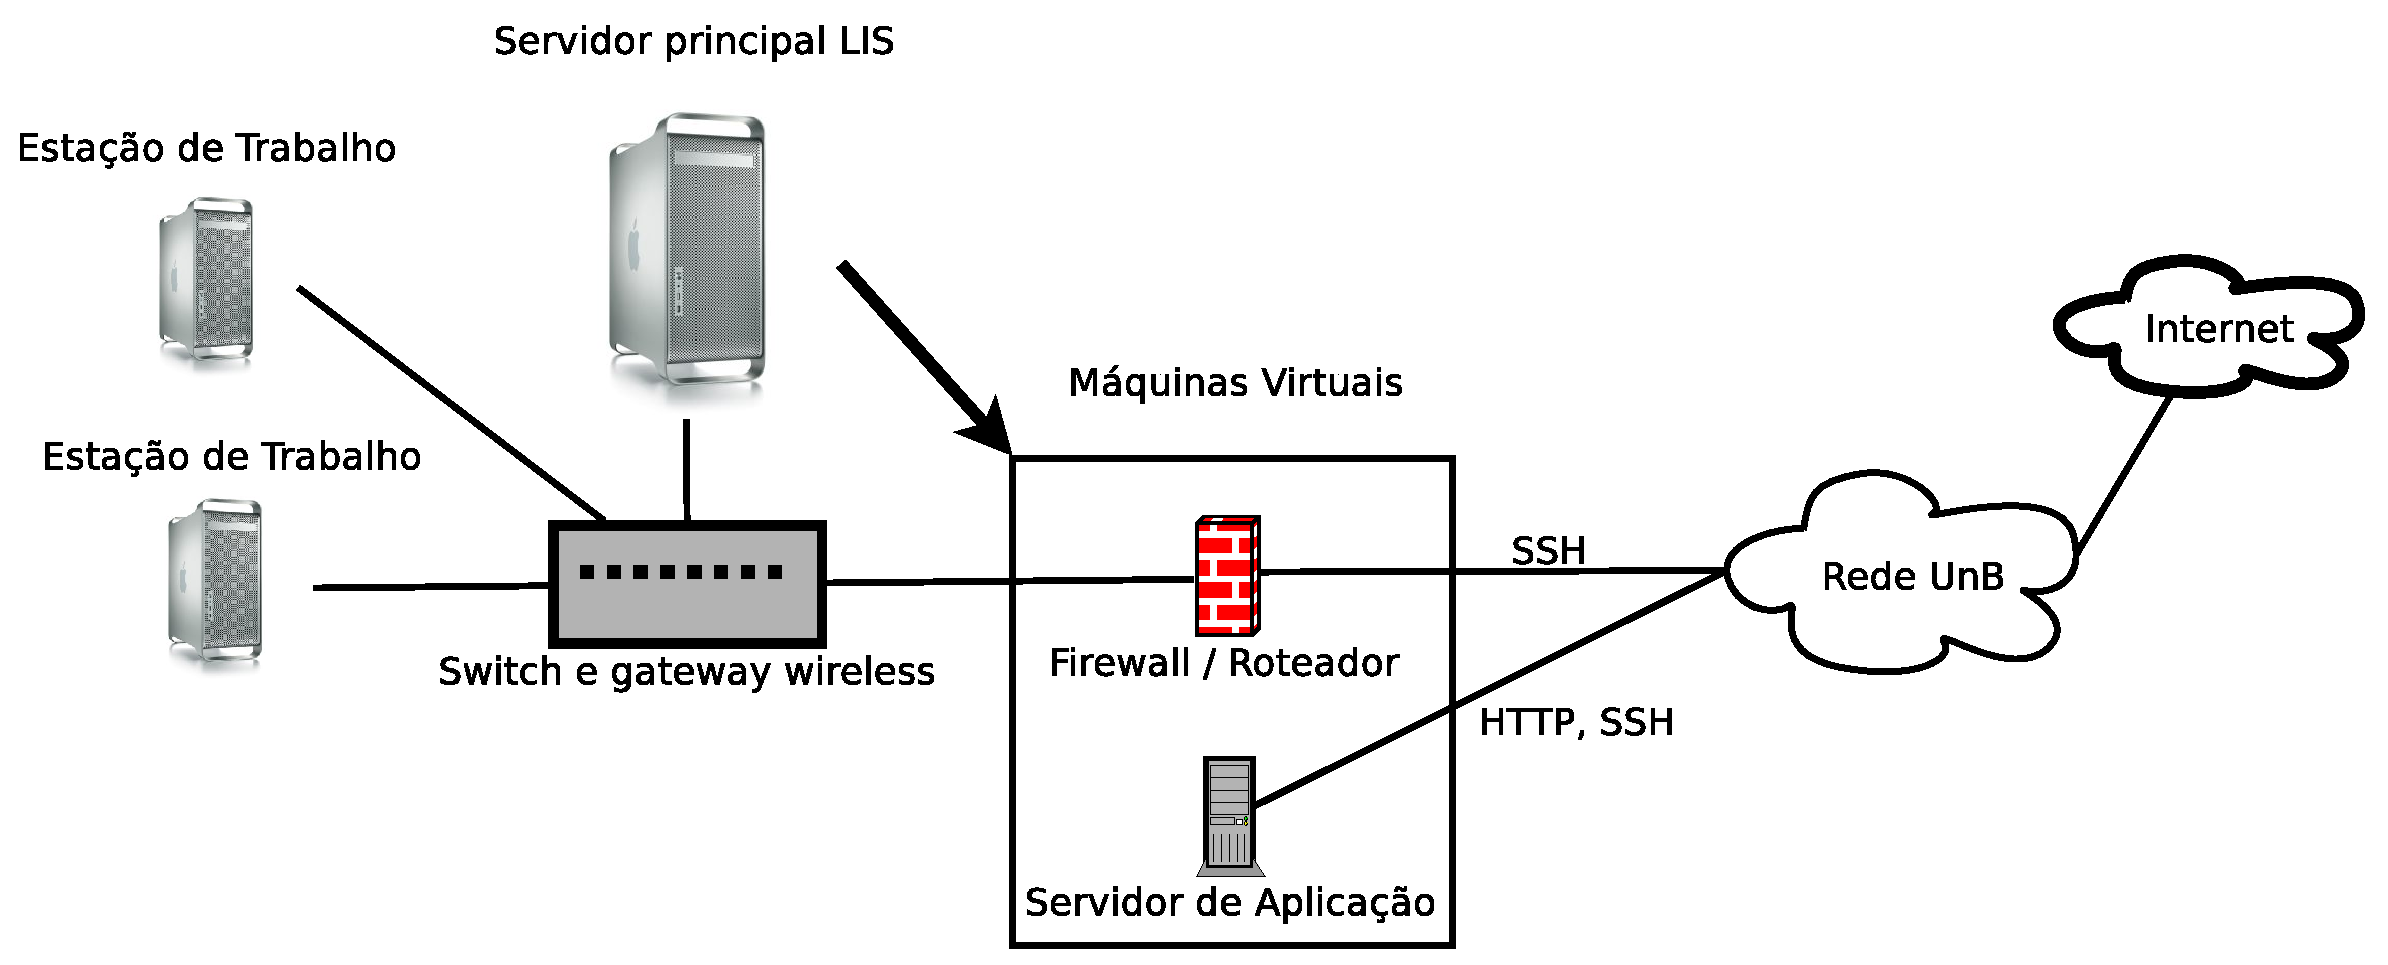
\includegraphics[width=15cm]{figuras/lis_rede.eps}
	\caption{Rede LIS}
	\label{lis_rede}
\end{figure}

O LPH foi utilizado para captura de dados de marcha humana. Este laboratório está equipado para coletar dados de plataformas de força, eletromiógrafos e de marcadores posicionados no corpo do paciente através de câmeras de vídeo (\emph{Motion Capture} - MOCAP). Para este trabalho foi utilizado o software \emph{QTM 3.2} da \emph{Qualisys}. 

\section[DELIMITAÇÃO DO ESTUDO]{DELIMITAÇÃO DO ESTUDO}

Este trabalho tem como foco estabelecer uma metodologia de desenvolvimento inicial a um sistema de análise e simulação de marcha. 
Ele não busca ser extensivo o suficiente para criar um produto pronto para o mercado, mas pretende, através da implementação de funcionalidades reais, estabelecer uma arquitetura mínima e funcional que sirva de base para a construção do sistema. 
Como consequência, o projeto também integra os principais componentes desta arquitetura, por exemplo, o serviço de banco de documentos, com a \emph{Application Program Interface} (API) \emph{web}.
Um software como este, robusto o suficiente para ser viável no mercado, seria muito caro. 
Por exemplo, um desenvolvedor sênior no mercado de Brasília, não custaria menos de R\$ 100.000,00 por ano para uma empresa. 


\section[VISÃO]{VISÃO} 
Apesar deste trabalho ter um objetivo específico e delimitado, dele nasce um projeto maior, cuja visão é o desenvolvimento de um software como serviço para análise e simulação de marcha, utilizando o estado da arte em técnicas para este fim. 
O software deve ser construído utilizando-se métodos ágeis e terá uma arquitetura adaptável que permita evolução contínua.

A estratégia é lançar a versão inicial do software como projeto de código livre, conseguir parceiros e procurar um modelo de negócio sustentável para mantê-lo.

\section[MODELO DE GESTÃO]{MODELO DE GESTÃO}
O software terá um modelo de gestão baseado no método \emph{SCRUM}, como definido em \ref{scrum_sec}.
O método não é adotado na plenitude, sendo adaptado segundo as limitações de recursos do projeto.

Nesta fase inicial, o processo conta com um desenvolvedor, que também assume o papel de \emph{scrum master}, e um \emph{product owner}. 
Devido ao tamanho reduzido da equipe e da localização distinta dos membros, não há \emph{daily scrum}, mas problemas de trabalho cotidianos são resolvidos por telefone, \emph{email} ou mensagens instantâneas. 

O princípio de \emph{time boxing} é mantido. Ficou definido que o \emph{sprint} consiste do prazo de duas semanas. Ao final do \emph{sprint} uma reunião em duas fases é realizada. A primeira fase consiste na revisão do \emph{sprint} anterior. Já a segunda fase é o planejamento do próximo \emph{sprint}.

Um \emph{backlog} de produto é mantido. Na reunião de final de \emph{sprint} é criado um \emph{backlog} de \emph{sprint}. 
Os itens de \emph{backlog} são mantidos na forma de estórias de usuários, conforme \ref{user_stories_sec}.
Na Figura \ref{scrum_projeto} é apresentada a visão geral do processo.

\begin{figure}[ht]
	\centering
	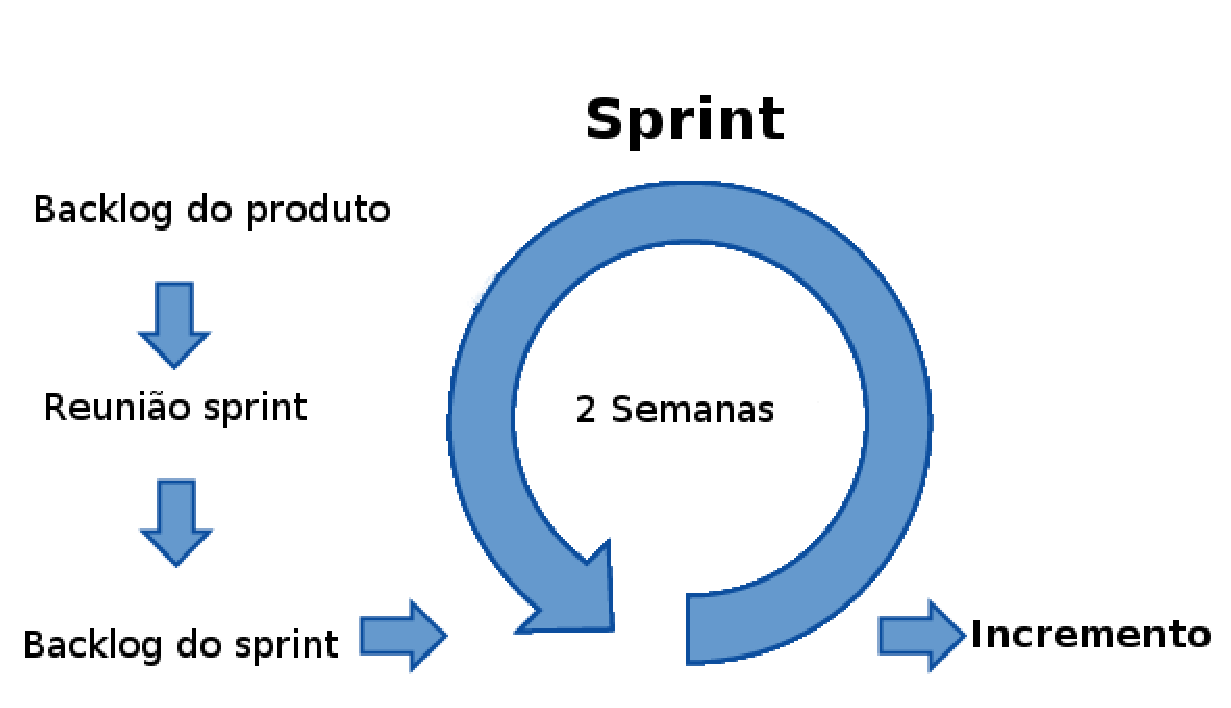
\includegraphics[width=15cm]{figuras/scrum_projeto.eps}
	\caption{Processo de desenvolvimento.}
	\label{scrum_projeto}
\end{figure}






\section[MODELO DE ARQUITETURA]{MODELO DE ARQUITETURA}

O modelo de arquitetura no seu nível mais elevado, pode ser visto como um modelo de três camadas, conforme a Figura \ref{camadas_arquitetura}.
\begin{figure}[ht]
	\centering
	\includegraphics[width=7cm]{figuras/camadas.eps}
	\caption{Camadas arquiteturais.}
	\label{camadas_arquitetura}
\end{figure}

A camada \emph{web} é responsável pela interação com o usuário. 
A camada \emph{Web API} é responsável pela lógica de negócio. 
A camada de base de documentos é responsável pela persistência dos dados da aplicação.


\subsection[CAMADA DE APLICAÇÃO WEB] {CAMADA DE APLICAÇÃO WEB}
Esta camada foi projetada para rodar em \emph{browsers} que suportam \emph{HTML} 5. 
Ela é desenvolvida usando-se \emph{Javascript}, \emph{CSS} e \emph{HTML}. 
Além disso, adotou-se o \emph{framework} de desenvolvimento \emph{web} \emph{AngularJS}, ver \ref{angularjs}. 

Como o projeto não possuía recursos adequados a criação de uma equipe de desenvolvimento \emph{web} completa, afim de se minimizar os problemas com \emph{design web}, optou-se por usar a biblioteca \emph{angular-material}, ver \ref{angular_material}. 

A Figura \ref{material_amostra}, mostra um exemplo de uma tela criada com as diretivas do angular-material. Note que todo o \emph{look and feel} da tela é determinado pelo comportamento padrão da biblioteca.

\begin{figure}[H]
	\centering
	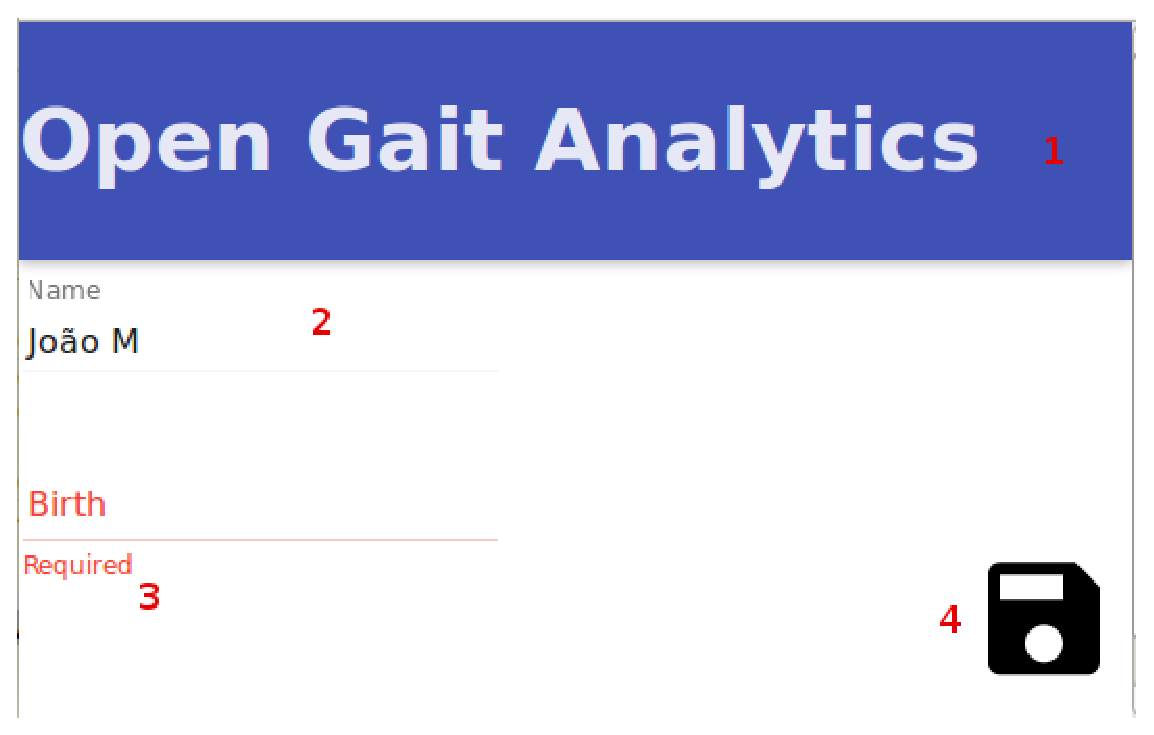
\includegraphics[width=9cm]{figuras/material_amostra.eps}
	\caption[Exemplo de uma tela criada com \emph{angular-material}.]{Exemplo de uma tela criada com \emph{angular-material}. 1) Diretiva \emph{md-toolbar}; 2) Diretiva \emph{md-input-container}; 3) Diretiva \emph{ng-messages} em conjunto com a \emph{md-input-container}; 4) Diretiva \emph{md-button}.}
	\label{material_amostra}
\end{figure}

\textbf{ORGANIZAÇÃO DO CÓDIGO FONTE}

\noindent
A criação de um ambiente de desenvolvimento \emph{web}, para um software de média para grande complexidade, não é uma tarefa trivial de ser resolvida.
É necessário criar padrões de organização de arquivos, configurar e instalar pacotes de software para desenvolvimento, testes, implantação, construção de \emph{builds}, entre outros.
Para facilitar esta tarefa, optou-se em utilizar o projeto \emph{angular-seed}, ver \ref{angular_seed}.
A ideia deste projeto é servir de esqueleto de projetos \emph{web} que utilizam o \emph{framework} \emph{AngularJS}.
Para usar este projeto, basta cloná-lo diretamente do seu repositório \emph{git} no \emph{site} github.com, conforme o comando abaixo.
\lstset{language=bash}
\begin{lstlisting}[frame=single]
git clone https://github.com/angular/angular-seed.git
\end{lstlisting}

\textbf{VISÃO ARQUITETURAL DA CAMADA \emph{WEB}}


\noindent
A Figura \ref{camda_web} mostra o funcionamento e os padrões mínimos a serem seguidos para implementação da camada \emph{web}.

\begin{figure}[H]
	\centering
	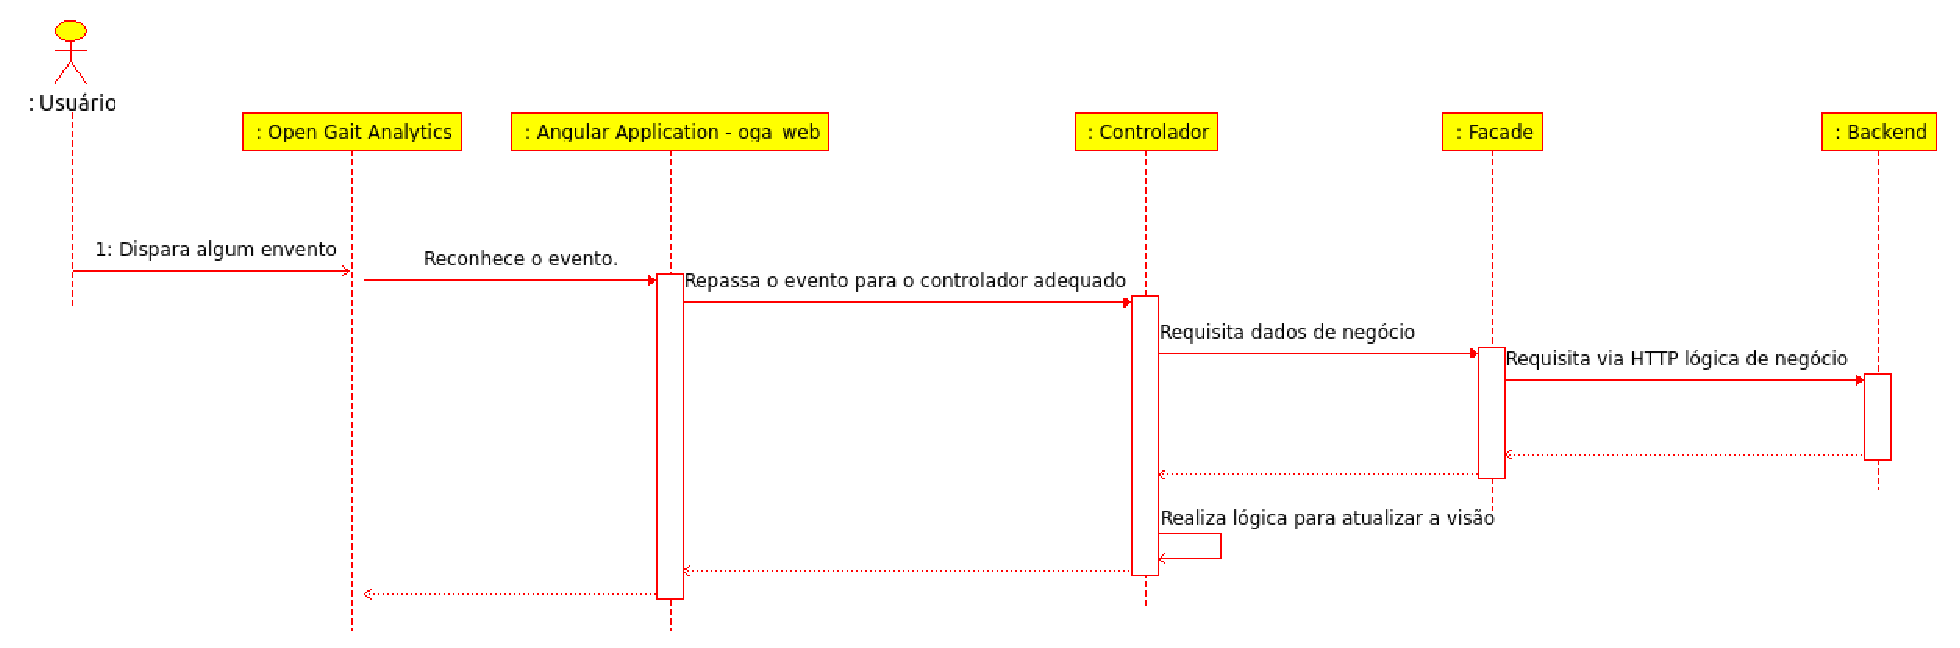
\includegraphics[width=17cm]{figuras/camada_web.eps}
	\caption{Camada \emph{web}.}
	\label{camda_web}
\end{figure}

Este esquema funciona da seguinte forma: O usuário usando seu \emph{browser}, acessa o \emph{site} do software. 
Ao realizar qualquer evento na aplicação, por exemplo, clicar num botão, ou selecionar um item em uma lista de seleção, a aplicação \emph{angularjs} detecta o evento e seleciona um componente de software chamado controlador. 
Existem vários destes controladores no sistema, cada evento do usuário é redirecionado para um que seja adequado.
No controlador é onde grande parte da programação acontece. 
Ele é associado a um \emph{template HTML}. 
Este template funciona como componente de apresentação para o usuário, e é o que o controlador manipula para mostrar informações ao usuário.
Quando o controlador precisa executar lógica de negócio, ou requisitar dados persistidos, ele deve chamar um componente do tipo \emph{Facade}. 
A aplicação \emph{web} roda no \emph{browser} do usuário e não persiste dados nem executa lógica de negócio. 
Este é um estilo arquitetural escolhido para o projeto.
A \emph{Facade} é um \emph{proxy} que se comunica com um \emph{backend} via HTTP no estilo \emph{REST} de comunicação via \emph{web}.

A Figura \ref{web_components}, mostra um exemplo de componentes escritos em \emph{JavaScript} respondendo a um evento disparado pelo usuário. 
Este evento poderia ser oriundo de um clique num botão ou na chamada de uma \emph{URL} específica. 
Depois de reconhecido o evento, no caso um pedido para ver a lista de pacientes, o componente \emph{PatientesCtrl} e o \emph{template patients.html} são carregado pelo \emph{framework AngularJS}. 
Neste momento o \emph{framework} acessa o componente \emph{PatientsFacade} através do seu método \emph{getPatients}. 
Este método invoca o método \emph{get} do componente \emph{\$HTTP} que faz parte do \emph{framework}.
Uma requisição é feita para o \emph{backend}, que retorna os dados no formato \emph{JSON}.
Finalmente, o \emph{framework} detecta a resposta e atualiza a tela para o usuário.

\begin{figure}[H]
	\centering
	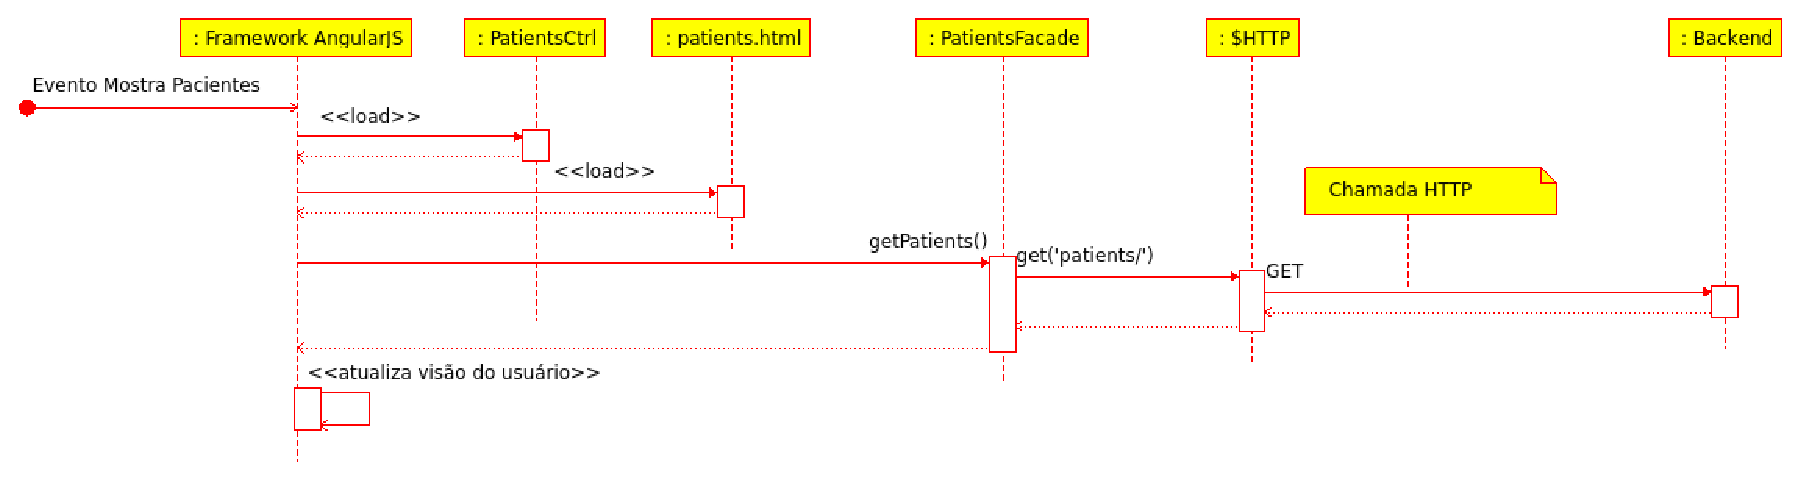
\includegraphics[width=17cm]{figuras/web_componentes.eps}
	\caption{Exemplo de componentes da camada \emph{web} funcionando juntos.}
	\label{web_components}
\end{figure}


\subsection{CAMADA \emph{REST WEB API}}

Esta é a camada responsável por expor toda a lógica de negócio e acesso a dados persistidos. Escolheu-se que esta camada fornece suas funções via \emph{web API} no estilo REST.
Uma das vantagens desta escolha é o alto desacoplamento, entre camada \emph{web} e lógica de negócio. 
Além disso, pode-se integrar mais facilmente a aplicação com outras, já que a lógica de negócio é toda exposta como \emph{API web}. 
Veja a seção \ref{servicos_rest} para um melhor entendimento deste estilo \emph{REST}.

\textbf{ORGANIZAÇÃO DO CÓDIGO FONTE}

\noindent
A Figura \ref{dir_api} mostra a configuração básica dos arquivos e diretórios da aplicação.

\begin{figure}[ht]
	\centering
	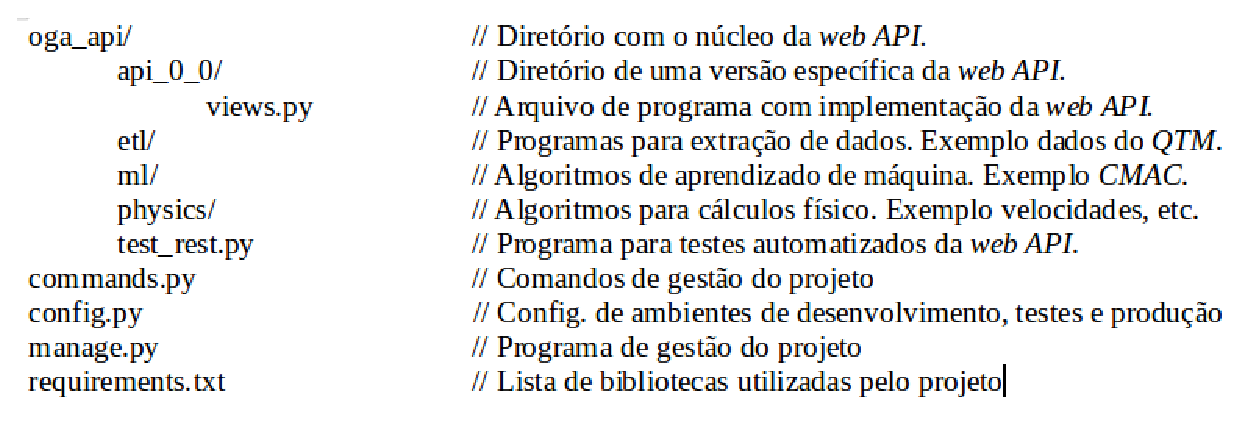
\includegraphics[width=15cm]{figuras/dir_api.eps}
	\caption{Organização do arquivos e diretórios da camada \emph{web API}.}
	\label{dir_api}
\end{figure}

A linguagem de programação \emph{Python} foi escolhida para implementar esta camada. Vários foram os motivos: a biblioteca \emph{Flask} para implementar a \emph{web API}, a biblioteca \emph{NumPy}, que é excelente para cálculos, comparável ao Matlab, a biblioteca \emph{Matplotlib} para criação de gráficos científicos, a baixa curva de aprendizado da linguagem, sua fama com desenvolvedores ao redor do mundo.

Para diminuir os problemas de ambientes, oriundos de um projeto complexo como este, optou-se por utilizar o programa \emph{virtualenv}. Este programa cria um ambiente \emph{python} virtual, baseado num arquivo de configuração. Isso faz com que todos os desenvolvedores envolvidos no projeto, possuam ambientes muito semelhantes.
Ao se clonar o projeto basta entrar no diretório da API e digitar o comando:
\lstset{language=bash}
\begin{lstlisting}[frame=single]
virtualenv env
\end{lstlisting}

Este comando irá criar uma diretório chamado \emph{env}. Para poder ativar o ambiente virtual é necessário o comado no unix:
\lstset{language=bash}
\begin{lstlisting}[frame=single]
. env/bin/activate
\end{lstlisting}

As bibliotecas necessárias a execução da aplicação estão listadas no arquivo \emph{requirements.txt}. Para instalá-las no novo ambiente virtual é necessário o comando:
\lstset{language=bash}
\begin{lstlisting}[frame=single]
pip install -r requirements.txt
\end{lstlisting}

Neste ponto, o código já pode ser editado e executado. Para facilitar um pouco as coisas, foi criado o programa \emph{manage.py}. Para rodar um servidor \emph{web} local respondendo na porta 5000, com fins de desenvolvimento, basta digitar o comando:
\lstset{language=bash}
\begin{lstlisting}[frame=single]
python manage.py runserver
\end{lstlisting}

Já para executar testes automatizados:
\lstset{language=bash}
\begin{lstlisting}[frame=single]
python manage.py test
\end{lstlisting}

Vale lembrar que o servidor \emph{MongoDB}, deve estar configurado, rodando e suas configurações editadas no arquivo \emph{config.py}.


\textbf{VISÃO ARQUITETURAL DA CAMADA \emph{REST WEB API}} 

\noindent
A Figura \ref{camada_api} mostra um \emph{blueprint} de como funciona e como deve ser desenvolvida esta camada.
\begin{figure}[ht]
	\centering
	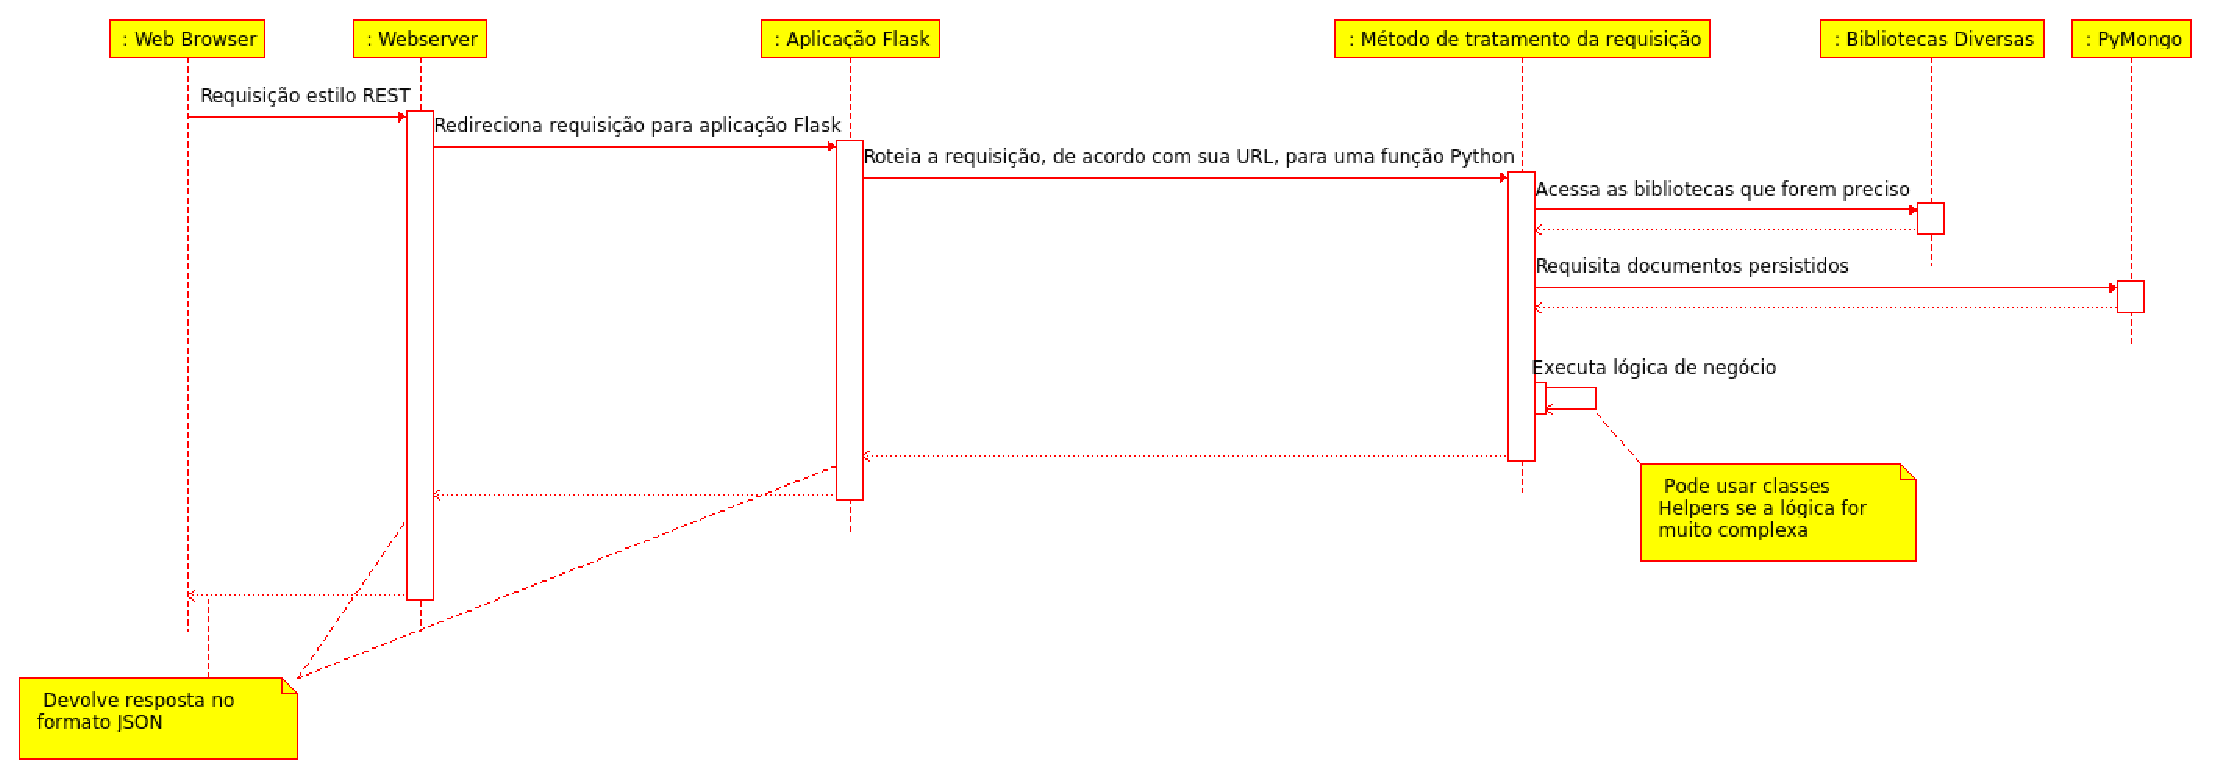
\includegraphics[width=15cm]{figuras/camada_api.eps}
	\caption{Camada \emph{REST WEB API}.}
	\label{camada_api}
\end{figure}

Tudo começa quando um \emph{browser web} faz uma requisição do tipo \emph{HTTP} a um servidor \emph{web}. 
O servidor \emph{web} identifica se a requisição é para a aplicação \emph{flask} do sistema em questão. 
Se for, esta requisição é repassada para a aplicação \emph{flask}. 
Agora as coisas começam a ficar mais interessantes. 
A aplicação \emph{flask} analisa a \emph{URL} da requisição, verifica o método da requisição e repassa os dados da requisição, num formato amigável ao \emph{python}, para uma função \emph{python}. 
Por padrão os parâmetros das requisições via método \emph{``GET"} são repassadas ao \emph{python} como \emph{string}. 
Para os demais métodos, padronizou-se receber o \emph{payload} da requisição \emph{HTTP}, como objetos JSON, que são facilmente convertidos para dicionários \emph{python}.

São nas funções \emph{python}, que tratam as requisições, que a lógica de negócio é executada. 
Aqui bibliotecas como a \emph{NumPy} podem ser chamadas, ou mesmo bibliotecas criadas pelos desenvolvedores da aplicação. 
É a partir deste ponto que dados podem ser acessados do banco de documentos pela biblioteca \emph{PyMongo}. 
Ao final da execução uma resposta é gerada no formato \emph{JSON} para que seja consumida pela camada \emph{web}.

A Figura \ref{webapi_componentes}, mostra um exemplo de componentes escritos em \emph{Python}, tratando uma requisição \emph{HTTP}, no caso uma chamada a \emph{URL http://<<myurl>>/patient}.
Depois que o servidor \emph{web} repassou a requisição para a aplicação que usa o \emph{framework Flask}, o \emph{framework} executa sua rotina de roteamento e descobre qual função \emph{Python}, contida no componente \emph{views},  deve ser executada, no caso a função \emph{get\_patients}.
Esta função acessa um objeto do tipo \emph{DataBase}, pertencente a biblioteca \emph{PyMongo}, e executa o método \emph{find} da coleção \emph{patients} pertencente ao \emph{DataBase}.
O resultado desta chamada são os dados contidos no banco de dados retornados no formato \emph{BSON}.
O componente \emph{json\_util}, da biblioteca \emph{PyMongo}, tem seu método \emph{dumps} chamado.
Este método converte os dados de \emph{BSON} para \emph{JSON}.
Finalmente, o \emph{framework Flask} responde a requisição.


\begin{figure}[ht]
	\centering
	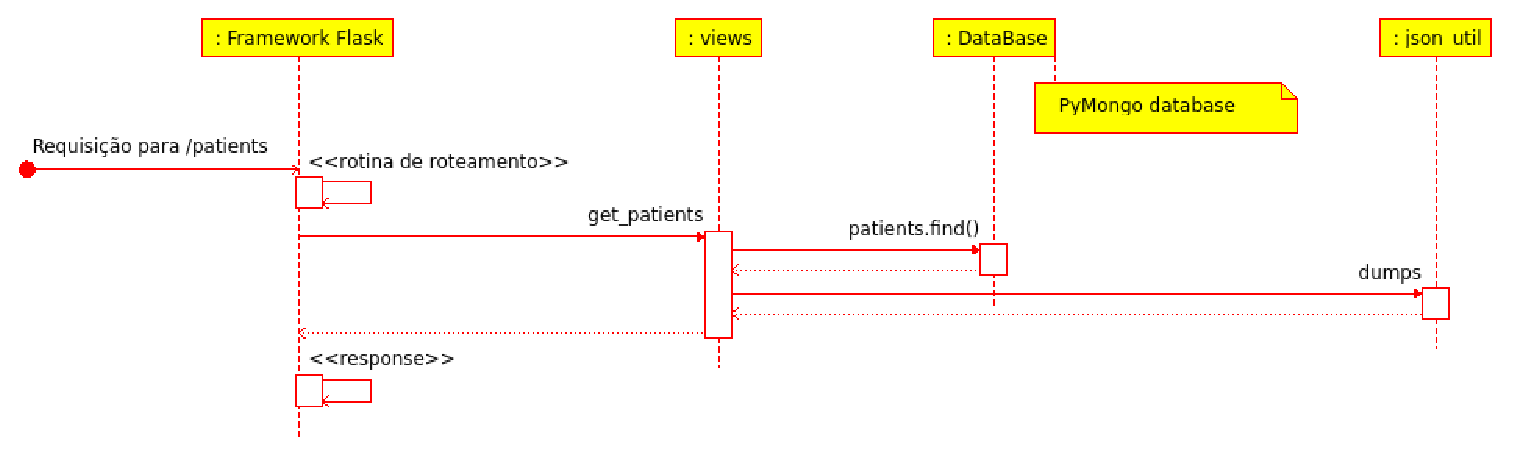
\includegraphics[width=17cm]{figuras/webapi_componentes.eps}
	\caption{Exemplo de requisição sendo tratada pela \emph{web api}.}
	\label{webapi_componentes}
\end{figure}

\subsection {CAMADA DE BASE DE DOCUMENTOS}

Para esta camada foi escolhido o banco de documentos \emph{MongoDB}, ver a seção \ref{mongodb_sec}. 
Há várias vantagens no uso desta tecnologia, mas a determinante foi a facilidade de uso e criação de estruturas de dados. 
No início do projeto, foi usado um banco de dados relacional e um \emph{framework} de mapeamento objeto-relacional. 
Devido a natureza altamente complexa dos dados, dados espaciais provindos de marcadores de superfície capturados por câmeras, eles são multidimensionais também. 
Sem dúvida isto ajudou a tornar possível criar esta primeira versão do software em tão pouco tempo.

A estrutura do banco da aplicação é mostrada na Figura \ref{mongo_oga}. 
O banco é composto por duas coleções: os dados dos pacientes na coleção \emph{patients} e os dados recuperados do \emph{QTM} \emph{positionals\_data}.

\begin{figure}[H]
	\centering
	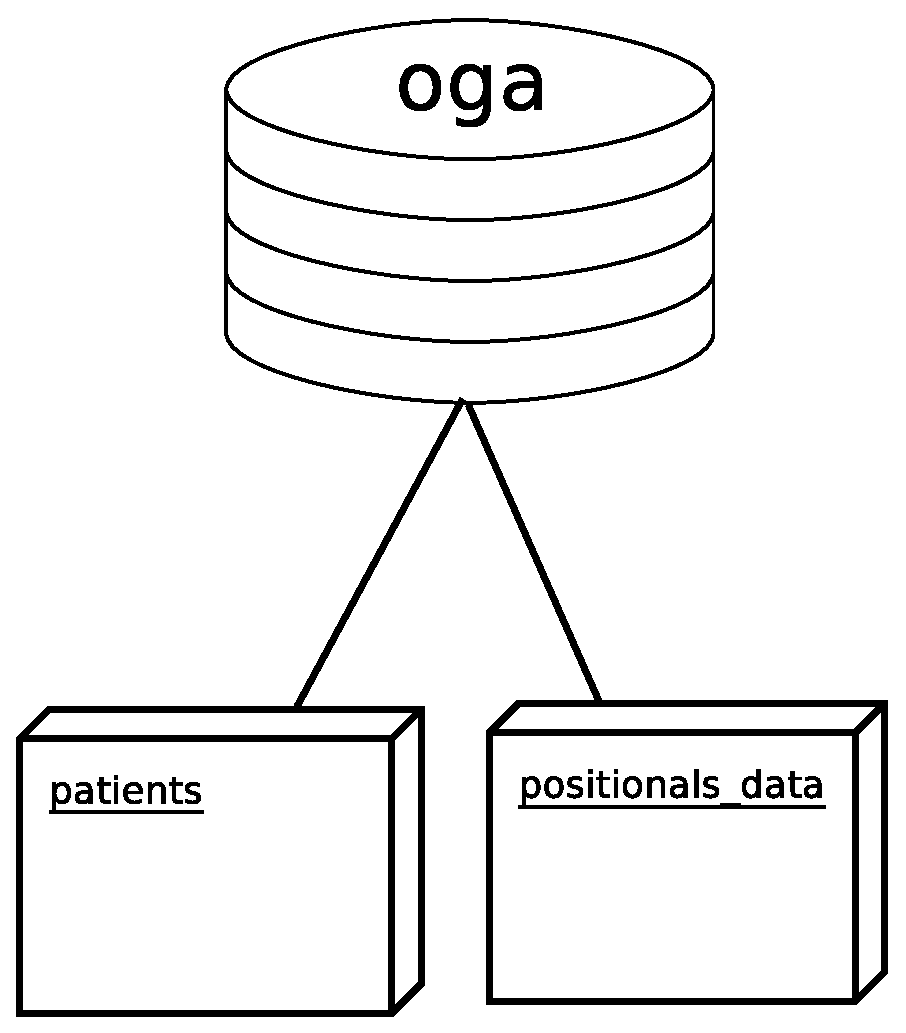
\includegraphics[width=5cm]{figuras/mongo_oga.eps}
	\caption{Banco de documentos da aplicação.}
	\label{mongo_oga}
\end{figure}

A Figura \ref{listagem2}  mostra um exemplo de documento da coleção \emph{patients}.
Já a Figura \ref{listagem3}  mostra um exemplo de documento da coleção \emph{positionals\_data}.

\begin{figure}[H]
	\centering
	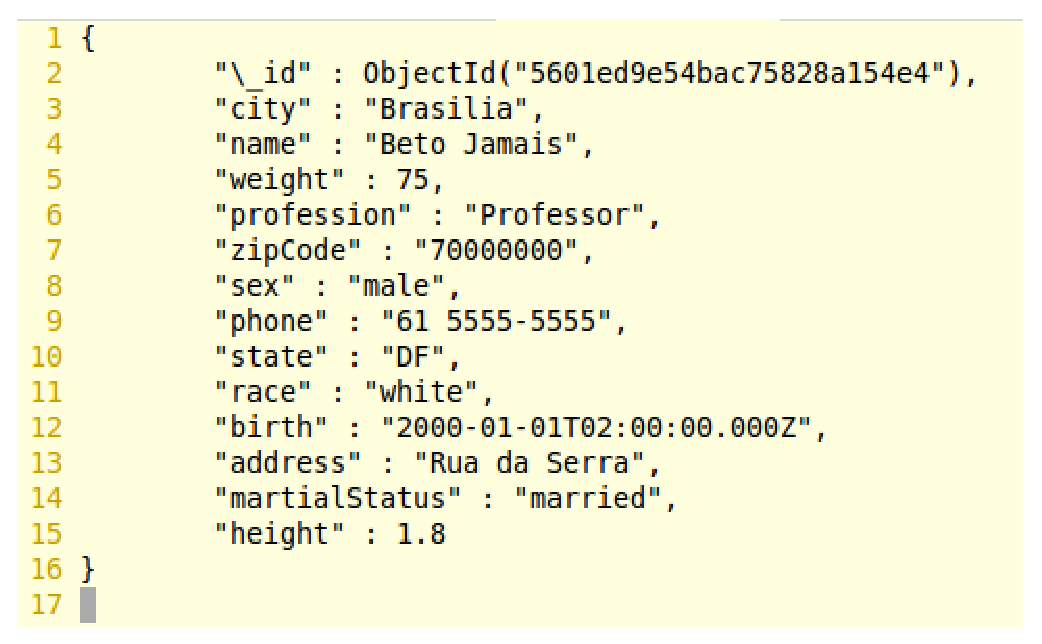
\includegraphics[width=10cm]{figuras/listagem2.eps}
	\caption{Documento da coleção \emph{patients}.}
	\label{listagem2}
\end{figure}

\begin{figure}[H]
	\centering
	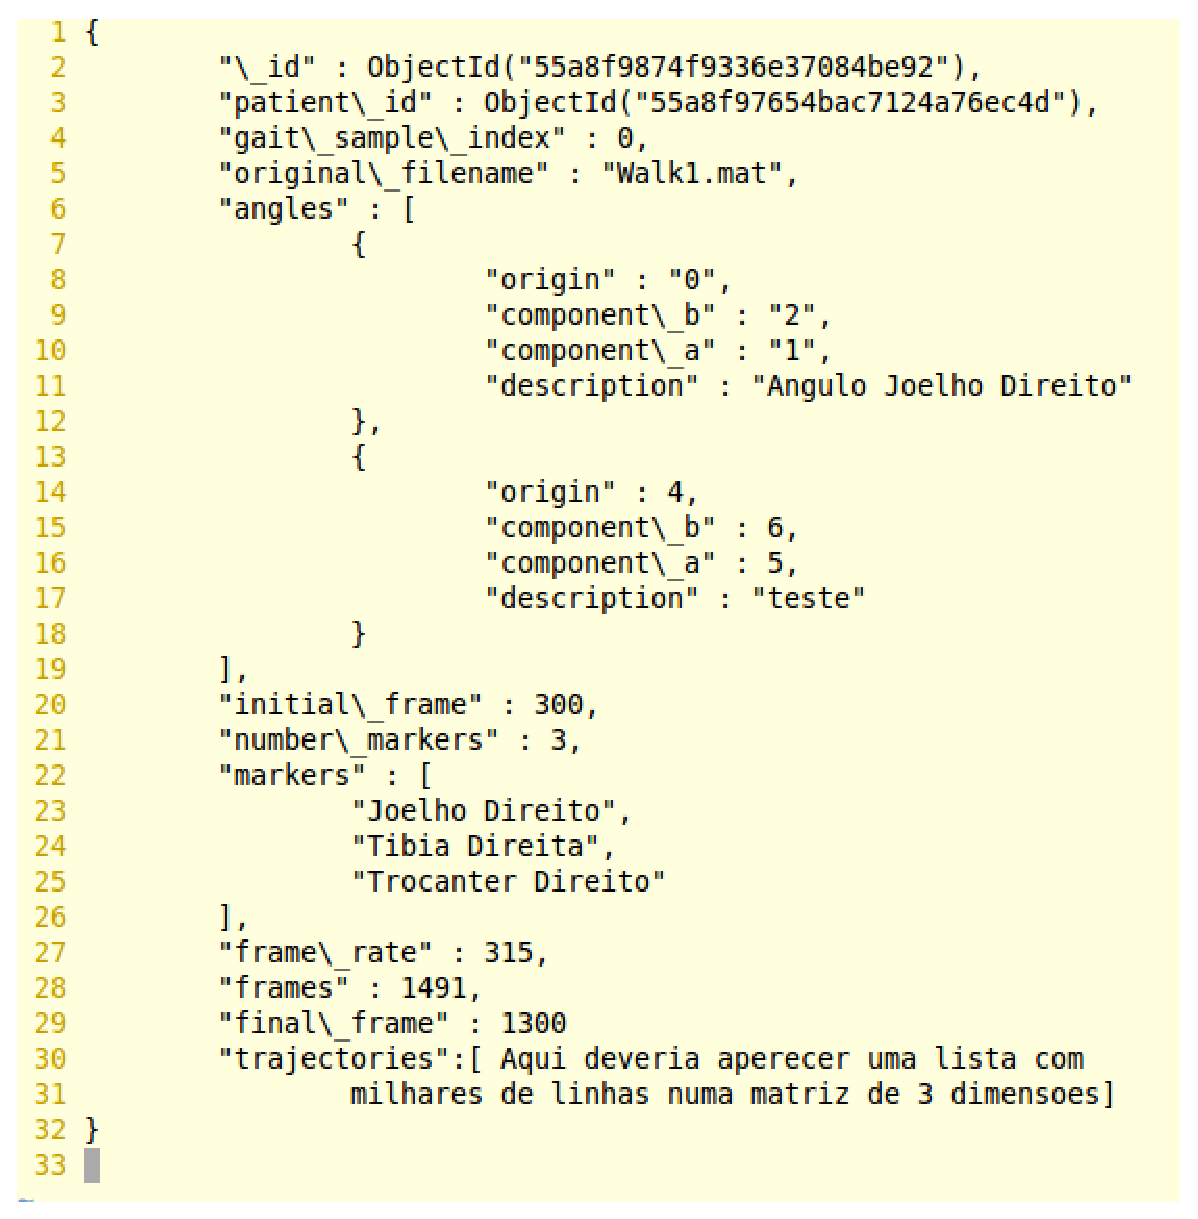
\includegraphics[width=10cm]{figuras/listagem3.eps}
	\caption{Documento da coleção \emph{positionals\_data}.}
	\label{listagem3}
\end{figure}




\begin{comment}
\section[FASES ESTUDO]{FASES DO ESTUDO}
\subsection[Coleta dos Dados]{\textbf{Coleta dos Dados}}
Os dados para o treinamento da RNA CMAC são dados cinemáticos, capturados através de \emph{motion capture}, utilizando-se de várias câmeras \emph{Qualisys Oqus MRI}, com marcadores passivos e pacote de software \emph(QTM 3.2) da \emph{Qualisys}. 
O sistema utilizado suporta até 74 canais, ou marcadores simultâneos.

O projeto no qual ocorreu a coleta foi aprovado pelo Comitê de Ética da Faculdade de Saúde da UnB, processo N11911/12 (ver Anexo \ref{anexo1}).

A Figura \ref{coleta_dados} mostra o processo para coleta de dados.

\begin{figure}[ht]
 \centering
 \includegraphics[width=4cm]{figuras/coleta_dados.eps}
 \caption{Fluxo de coleta de dados.}
 \label{coleta_dados}
\end{figure}

Primeiro deve-se definir o voluntário da coleta e determinar o dia para este processo. 
Além disso, também é necessário definir quais os pontos no corpo do voluntário devem ser mapeados. 
Também se devem distribuir os marcadores em várias posições ao longo das pernas. 
Como só a flexão e a extensão dos joelhos interessam para este trabalho, utilizam-se somente marcadores nas tíbias, joelhos e trocânteres das duas pernas.

O próximo passo se refere ao voluntário, isto é, ele deve repetir um ciclo de marcha confortável de aproximadamente 5 segundos, por 5 vezes na frente das câmeras.

Quanto aos dados, estes devem ser convertidos para formato adequado à linguagem \emph{Octave}, que é a mesma opção para converter para o \emph{MATLAB}. Esta opção é própria do \emph{QTM}. 
Além da conversão é necessário definir o nome de cada item na matriz de dados coletados. 
Cada coluna desta matriz representa um marcador, são estes pontos que devem ser nomeados. 
Por exemplo, coluna 1 igual ao trocânter direito. 
O número que o QTM atribui internamente ao marcador é a posição do marcador na matriz. 
Este número é chamado dentro do QTM de canal. 
Os dados trazem variáveis espaciais e o erro, com respeito à posição (X, Y, Z) dos marcadores.

A disposição que os dados obtidos neste processo se apresentam, é mostrado na Figura \ref{dados_qtm}.

\begin{figure}[ht]
 \centering
 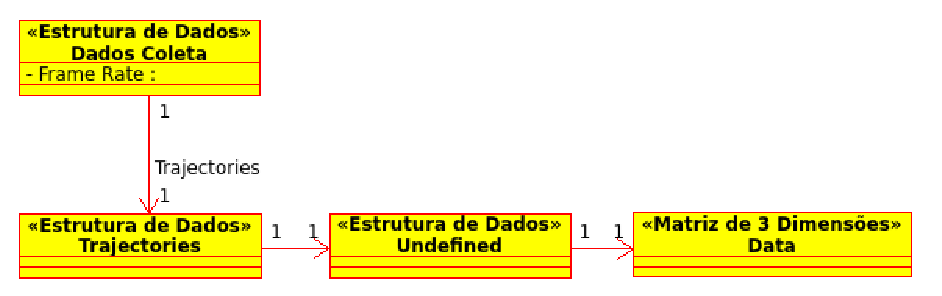
\includegraphics[width=15cm]{figuras/dados_qtm.eps}
 \caption{Dados disponibilizados pelo QTM.}
 \label{dados_qtm}
\end{figure}

Os dados que interessam são o \emph{Frame Rate} e o \emph{Data}.
São retornados vários dados, mas os de interesse para o projeto são os que estão na Figura \ref{dados_qtm}. 
O \emph{Frame Rate} é a taxa de coleta dos dados e está em segundos. 
A matriz de 3 dimensões está disposta da seguinte forma:
\begin{enumerate}
	\item A primeira dimensão é 74 e representa o número de canais do sistema de coleta;
	\item A segunda dimensão é 4 e representa a posição num plano 3D (X, Y, Z) do marcador, mais o erro;
	\item A terceira dimensão é número de frames coletados numa caminhada específica. Este número é variável.
\end{enumerate}



\subsection[Extração e transformação dos dados]{\textbf{Extração e transformação dos dados}}
Com os dados necessários disponibilizados no formato adequado é possível fazer os cálculos de angulações, velocidades angulares e acelerações angulares dos joelhos. Os casos de uso para esta fase são:
\begin{figure}[ht]
	\centering
	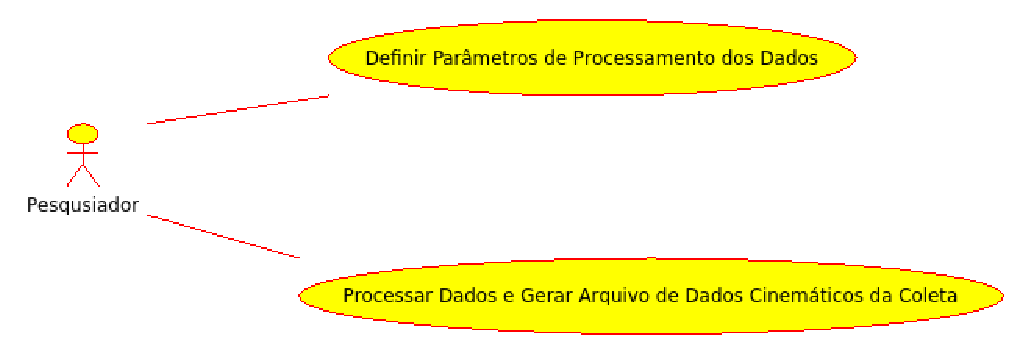
\includegraphics[width=15cm]{figuras/extracao_coleta.eps}
	\caption{Caso de uso para extração e transformação de dados}
	\label{extracao_coleta}
\end{figure}

O caso de uso Definir Parâmetros de Processamento dos Dados, definido na Figura \ref{extracao_coleta}, consiste em se definir os dados necessários para que depois seja possível processar os dados coletados. 
Estes dados são os definidos na Figura \ref{estrutura_dados}. 
O valor dos 6 primeiros atributos da estrutura de dados Configuração do Processamento, são os canais usados no QTM para tais marcadores.
\begin{figure}[ht]
	\centering
	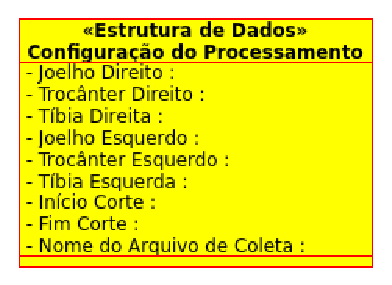
\includegraphics[width=7.5cm]{figuras/estrutura_dados.eps}
	\caption{Dados para processamento da coleta.}
	\label{estrutura_dados}
\end{figure}

O caso de uso Processar Dados e Gerar Arquivos de Dados Cinemáticos, definido na Figura \ref{extracao_coleta}, da coleta deve obedecer o processo da Figura \ref{tratamento_dados}.
\begin{figure}[ht]
	\centering
	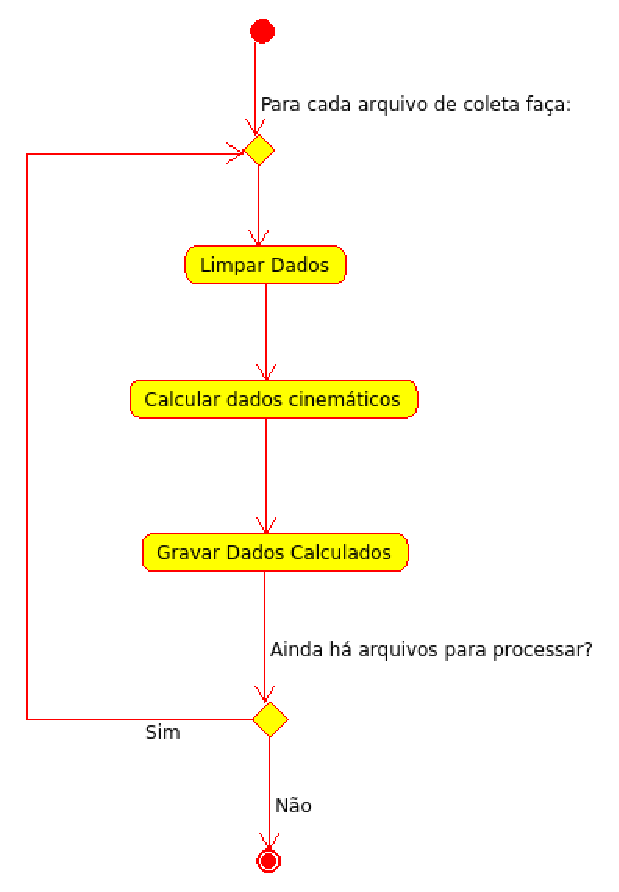
\includegraphics[width=10cm]{figuras/tratamento_dados.eps}
	\caption{Processo de tratamento dos dados.}
	\label{tratamento_dados}
\end{figure}

A limpeza dos dados consiste em retirar os dados desnecessários, como marcadores não desejados e retirada de frames do início e/ou final de um arquivo de coleta, que não estejam no ciclo de marcha confortável. 

Os cálculos realizados devem ser as velocidades instantâneas, velocidades angulares e acelerações angulares. 
Velocidades instantâneas dos joelhos são calculadas conforme a Equação \ref{velocidade}.
\begin{equation}
	\label{velocidade}
	\vec{\nu} = (\vec{a}-\vec{b})/t 
\end{equation}

A variável $\vec{a}$  é a posição (X, Y, Z) do joelho em uma determinada leitura sequencial dos dados coletados. 
A variável $\vec{b}$ é a próxima posição (X, Y, Z) da sequência. $t$ é o \emph{frame rate} definido nos dados da coleta.

Para o cálculo das angulações dos joelhos, primeiro os marcadores destes devem ser transladados para uma origem, assim é possível se usar a Equação 5 como descrita em \citeonline{Edwards2006}. 
Para tal, usam-se as Equações \ref{trocanter}, \ref{joelho} e \ref{tibia}.
\begin{equation}
	\label{trocanter}
	\vec{t_{r0}} = \vec{t_r} - \vec{j}
\end{equation}
\begin{equation}
	\label{joelho}
	\vec{j_0} = \vec{j} - \vec{j}
\end{equation}
\begin{equation}
	\label{tibia}
	\vec{t_{b0}} = \vec{t_b} - \vec{j}
\end{equation}

$\vec{t_{r0}}$ é o vetor que representa a posição de um trocânter $\vec{t_r}$, transladado para a nova origem.
$\vec{j}$ é vetor da posição do joelho.
$\vec{j_0}$ é a nova origem, que nada mas é que o joelho transladado para a posição $(0,0,0)$. 
$\vec{t_{b0}}$ é a posição da tíbia $\vec{t_b}$ transladada para a origem.
A translação de vetores é documentada em \citeonline{Poole2011}.

Agora que se tem os pontos transladados para uma origem, pode-se usar a Equação \ref{ang_joe} para o cálculo do ângulo $\theta$ do joelho.
\begin{equation}
	\label{ang_joe}
	\theta =
		cos^{-1} 
		\frac
		{
			\vec{t_{r0}} \cdot \vec{t_{b0}}
		}
		{
			\left \| \vec{t_{r0}} \right \|
			\cdot
			\left \| \vec{t_{b0}} \right \|
		}
\end{equation}

O operador $\left \| \right \|$ é o cálculo da distância euclidiana, ou norma. Pode ser calculado, segundo \citeonline{Poole2011}, de acordo com a Equação \ref{norma}. Resumindo, é a raiz quadrada do produto interno de um vetor.
\begin{equation}
	\label{norma}
	\left \| \vec{u} \right \| = \sqrt{\vec{u}\cdot\vec{u}}
\end{equation}

A velocidade angular $\omega$ do joelho é calculada a partir da Equação \ref{vel_ang}.
\begin{equation}
	\label{vel_ang}
	\omega = (\theta_1 - \theta_2) / t
\end{equation}

A variável $\theta_1$ é o ângulo de um joelho num determinado frame. A variável $\theta_2$ é exatamente o ângulo do próximo frame. A variável $t$ é o \emph{frame rate}, oriundo dos dados da coleta.


A última etapa deste processo é a gravação dos dados para que possam ser usados pela RNA CMAC. 
Estes dados devem ser gravados num arquivo em formato texto. 
As linhas neste arquivo equivalem aos \emph{frames}. 
Cada coluna equivale às informações, na ordem em que aparecem, da estrutura de dados descrita na Figura \ref{dados_cinematicos}. 
\begin{figure}[ht]
	\centering
	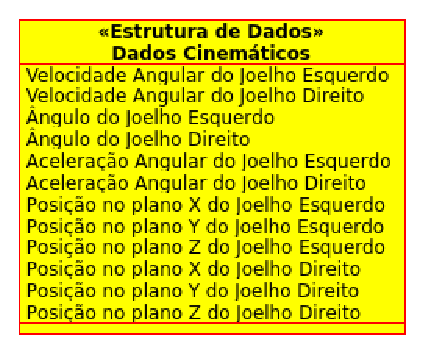
\includegraphics[width=7.5cm]{figuras/dados_cinematicos.eps}
	\caption{Dados Cinemáticos da Marcha}
	\label{dados_cinematicos}
\end{figure}

\subsection[Construção de uma RNA CMAC]{\textbf{Construção}}
\subsubsection{Modelo Geral}

A RNA CMAC proposta para este trabalho é resumida na Figura \ref{camac_resumida}.

\begin{figure}[ht]
	\centering
	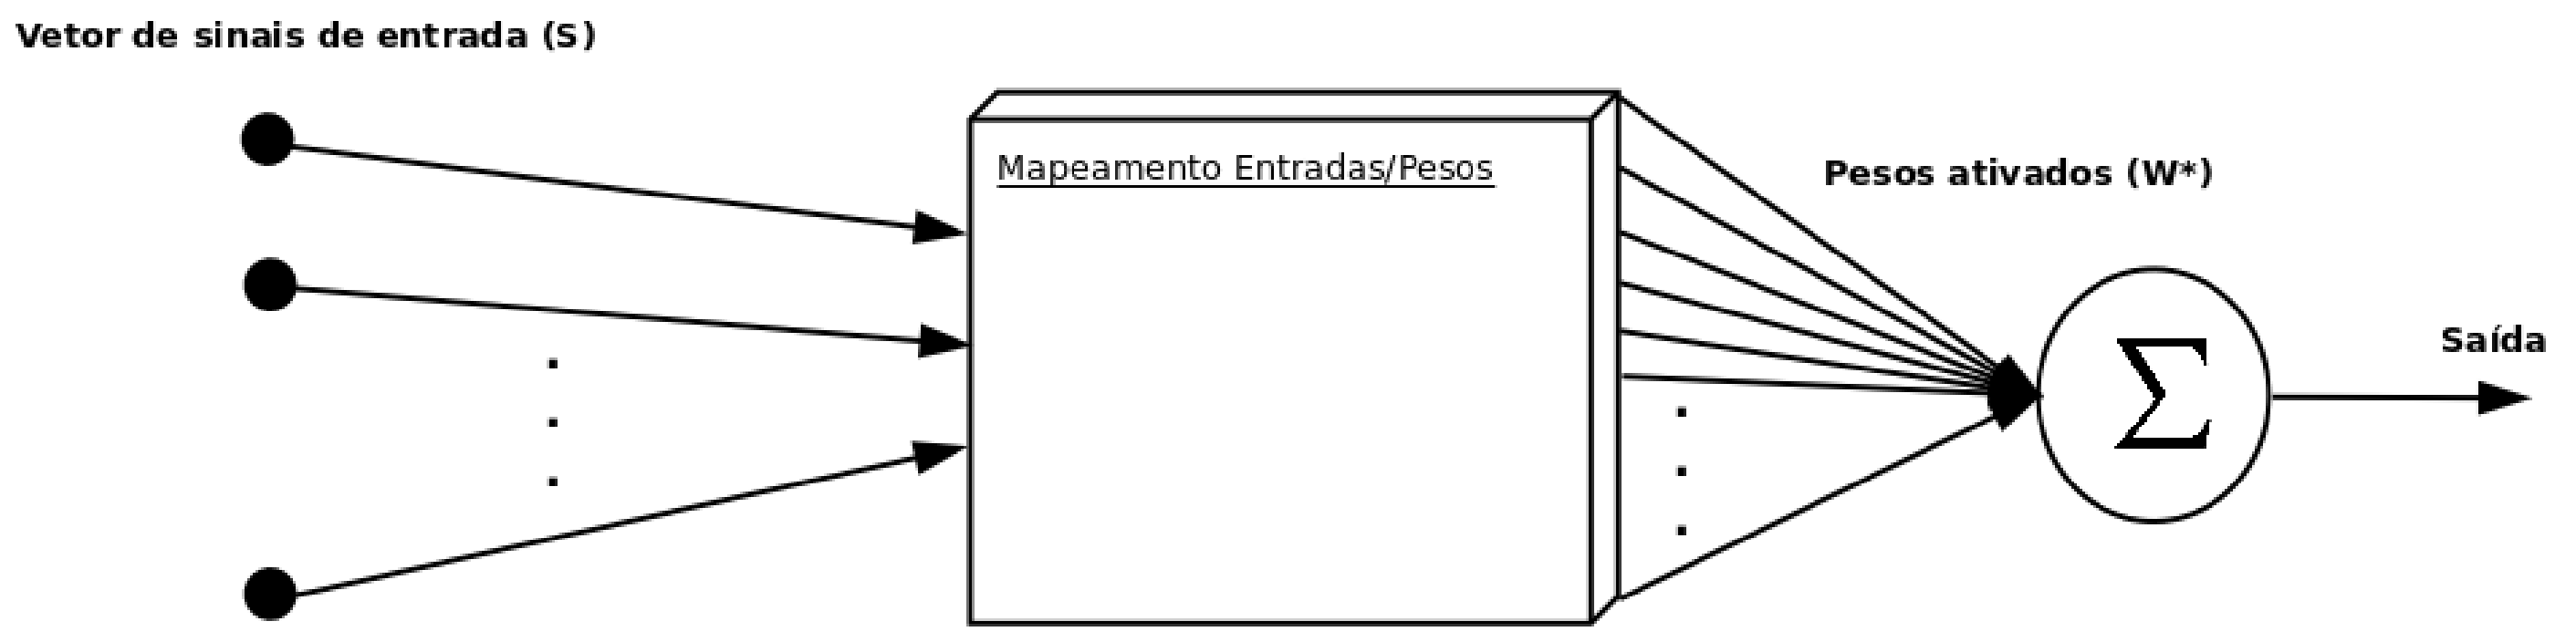
\includegraphics[width=15cm]{figuras/cmac_resumida.eps}
	\caption{CMAC resumida.}
	\label{camac_resumida}
\end{figure}

A variável $S$ é o vetor de sinais de entrada. 
Esses sinais são passados para um processo de mapeamento entre a entrada e um conjunto de pesos. 
Depois apenas os pesos ativados participam da somatória que é o sinal de saída. 

Para se calcular a saída da rede, primeiramente define-se o número de pesos $NW*$ a serem ativados.

O segundo passo é definir os possíveis valores para cada item do vetor de entradas $S$. A isto chama-se quantização. Por exemplo, se o primeiro item $s1$ de $S$ aceita valores entre $-1$ até $1$ e se quer $5$ valores possíveis, quantiza-se $s1$ conforme a Figura \ref{quantizacao}.
\begin{figure}[ht]
	\centering
	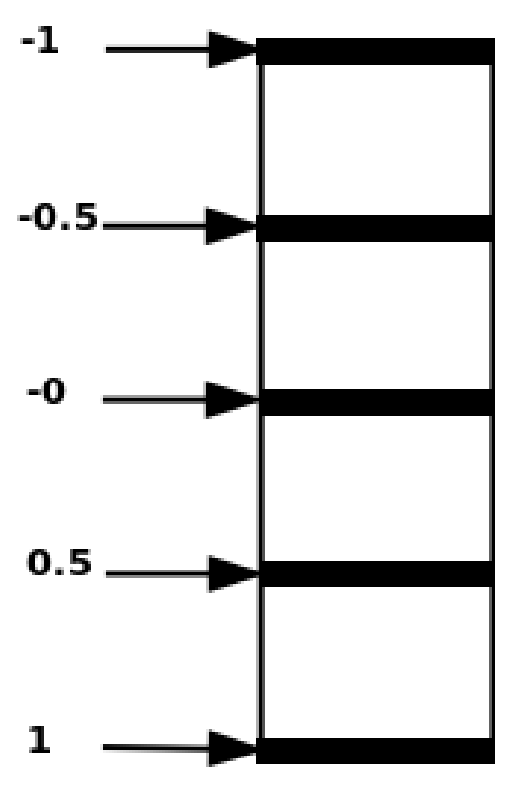
\includegraphics[width=5cm]{figuras/quatizacao.eps}
	\caption{Quantização de $s1$}
	\label{quantizacao}
\end{figure}

Isto significa que quaisquer que sejam os valores de $s1$ os mesmos devem ser convertidos para $-1$, $-0,5$, $0$, $0,5$ e $1$. 
Por exemplo, se o valor de s1 for $0,75$, será convertido para o valor $1$, se for $-0,75$ será o valor $0$ e se for $0,25$ será o valor $0,5$. À discretização dá-se o nome de resolução da CMAC.

O próximo passo é criar uma tabela para cada um dos sinais discretizados de entrada do vetor $S$.
Supondo que o vetor $S$ possui 2 sinais de entrada $s1$ e $s2$ e um número de ativações $NW*$ igual a 3, cria-se Tabela \ref{map_s1} e a Tabela \ref{map_s2}. 
Para facilitar o entendimento, irá se considerar os valores de $s1$ iguais aos inteiros de 1 até 6 e os valores de s2 iguais aos inteiros de 1 até 4.
\begin{table}[htb]
	\IBGEtab{%
		\caption{Mapeamento de $s1$}%
		\label{map_s1}
	}
	{%
		\begin{tabular}{cc}
			\toprule
			\textbf{Valores de $s1$} & \textbf{Mapeamento $m1$} \\
			\midrule
			1	&	0, 1, 2	\\
			\midrule
			2	&	3, 1, 2	\\
			\midrule
			3	&	3, 4, 3	\\
			\midrule
			4	&	3, 4, 5	\\
			\midrule
			5	&	6, 4, 6	\\
			\midrule
			6	&	6, 7, 5	\\
			\bottomrule
		\end{tabular}%
	}
	{%
		\fonte{Produzido pelo autor.}%
	}
\end{table}

\begin{table}[htb]
	\IBGEtab{%
		\caption{Mapeamento de $s2$}%
		\label{map_s2}
	}
	{%
		\begin{tabular}{cc}
			\toprule
			\textbf{Valores de $s2$} & \textbf{Mapeamento $m2$} \\
			\midrule
			1	&	0, 1, 2	\\
			\midrule
			2	&	3, 1, 2	\\
			\midrule
			3	&	3, 4, 3	\\
			\midrule
			4	&	3, 4, 5	\\
			\bottomrule
		\end{tabular}%
	}
	{%
		\fonte{Produzido pelo autor.}%
	}
\end{table}

Estas tabelas são criadas da seguinte forma:
O mapeamento consiste num número de itens igual a $NW*$, 3 no caso.
Este número é o número de pesos a serem ativados.
Para a primeira linha de cada uma das tabelas, atribui-se uma sequência de 3 valores inteiros começando com 0.
A próxima linha deve conter o próximo valor da sequência, 3, como primeiro item do mapeamento e continuar com os demais itens iguais aos da linha anterior. 
Na próxima linha, substitui-se o segundo item de mapeamento pelo próximo número da sequência, 4, mantendo-se os demais itens e assim sucessivamente.

Depois de mapeado cada valor de cada item de entrada, deve-se combinar os mapeamentos de acordo com a Tabela \ref{map_w}.
\begin{table}[htb]
	\IBGEtab{%
		\caption{Mapeamento para os pesos $W$}%
		\label{map_w}
	}
	{%
		\begin{tabular}{ccccc}
			\toprule
			\begin{tabular}{c}
				\textbf{$s2$}	\\
				\textbf{$s1$}	\\
			\end{tabular} 
			& \textbf{1} & \textbf{2} & \textbf{3} & \textbf{4} \\
			\midrule
			\textbf{1}	& 1 & 2 & 3 & 4 \\
			\bottomrule
		\end{tabular}%
	}
	{%
		\fonte{Produzido pelo autor.}%
	}
\end{table}

\end{comment}


\chapter[RESULTADOS]{\textbf {RESULTADOS}}

O software construído por este projeto, o \emph{Open Gait Analytics} versão 0.1, foi interamente construído pelo autor desta obra, e está liberado no site \url{https://github.com/rob-nn/open_gait_analytics}, sob a licença \emph{MIT}. Para saber mais sobre esta licença veja \ref{mit_sec}.
A intenção do autor é aumentar as chances de que futuras versões do software sejam construídas, não importando se serão comerciais ou gratuitas.
Importante frizar também que o software continuará sendo desenvolvido pelo autor nos próximos meses.

O software em si é composto por dois módulos que são apresentados na Figura \ref{tela1}. O principal objetivo neste momento é atrair pesquisadores da área de análise de marcha para o software. Por isso há o módulo simulação, no qual o pesquisador poderá simular sinais.
O módulo de análise visa atender tanto a pesquisadores, quanto a profissionais da área clínica. Neste momento o software é mais um protótipo funcional do que algo pronto para o mercado, portanto o uso por profissionais da área clínica não é recomendado ainda.

\begin{figure}[ht]
	\centering
	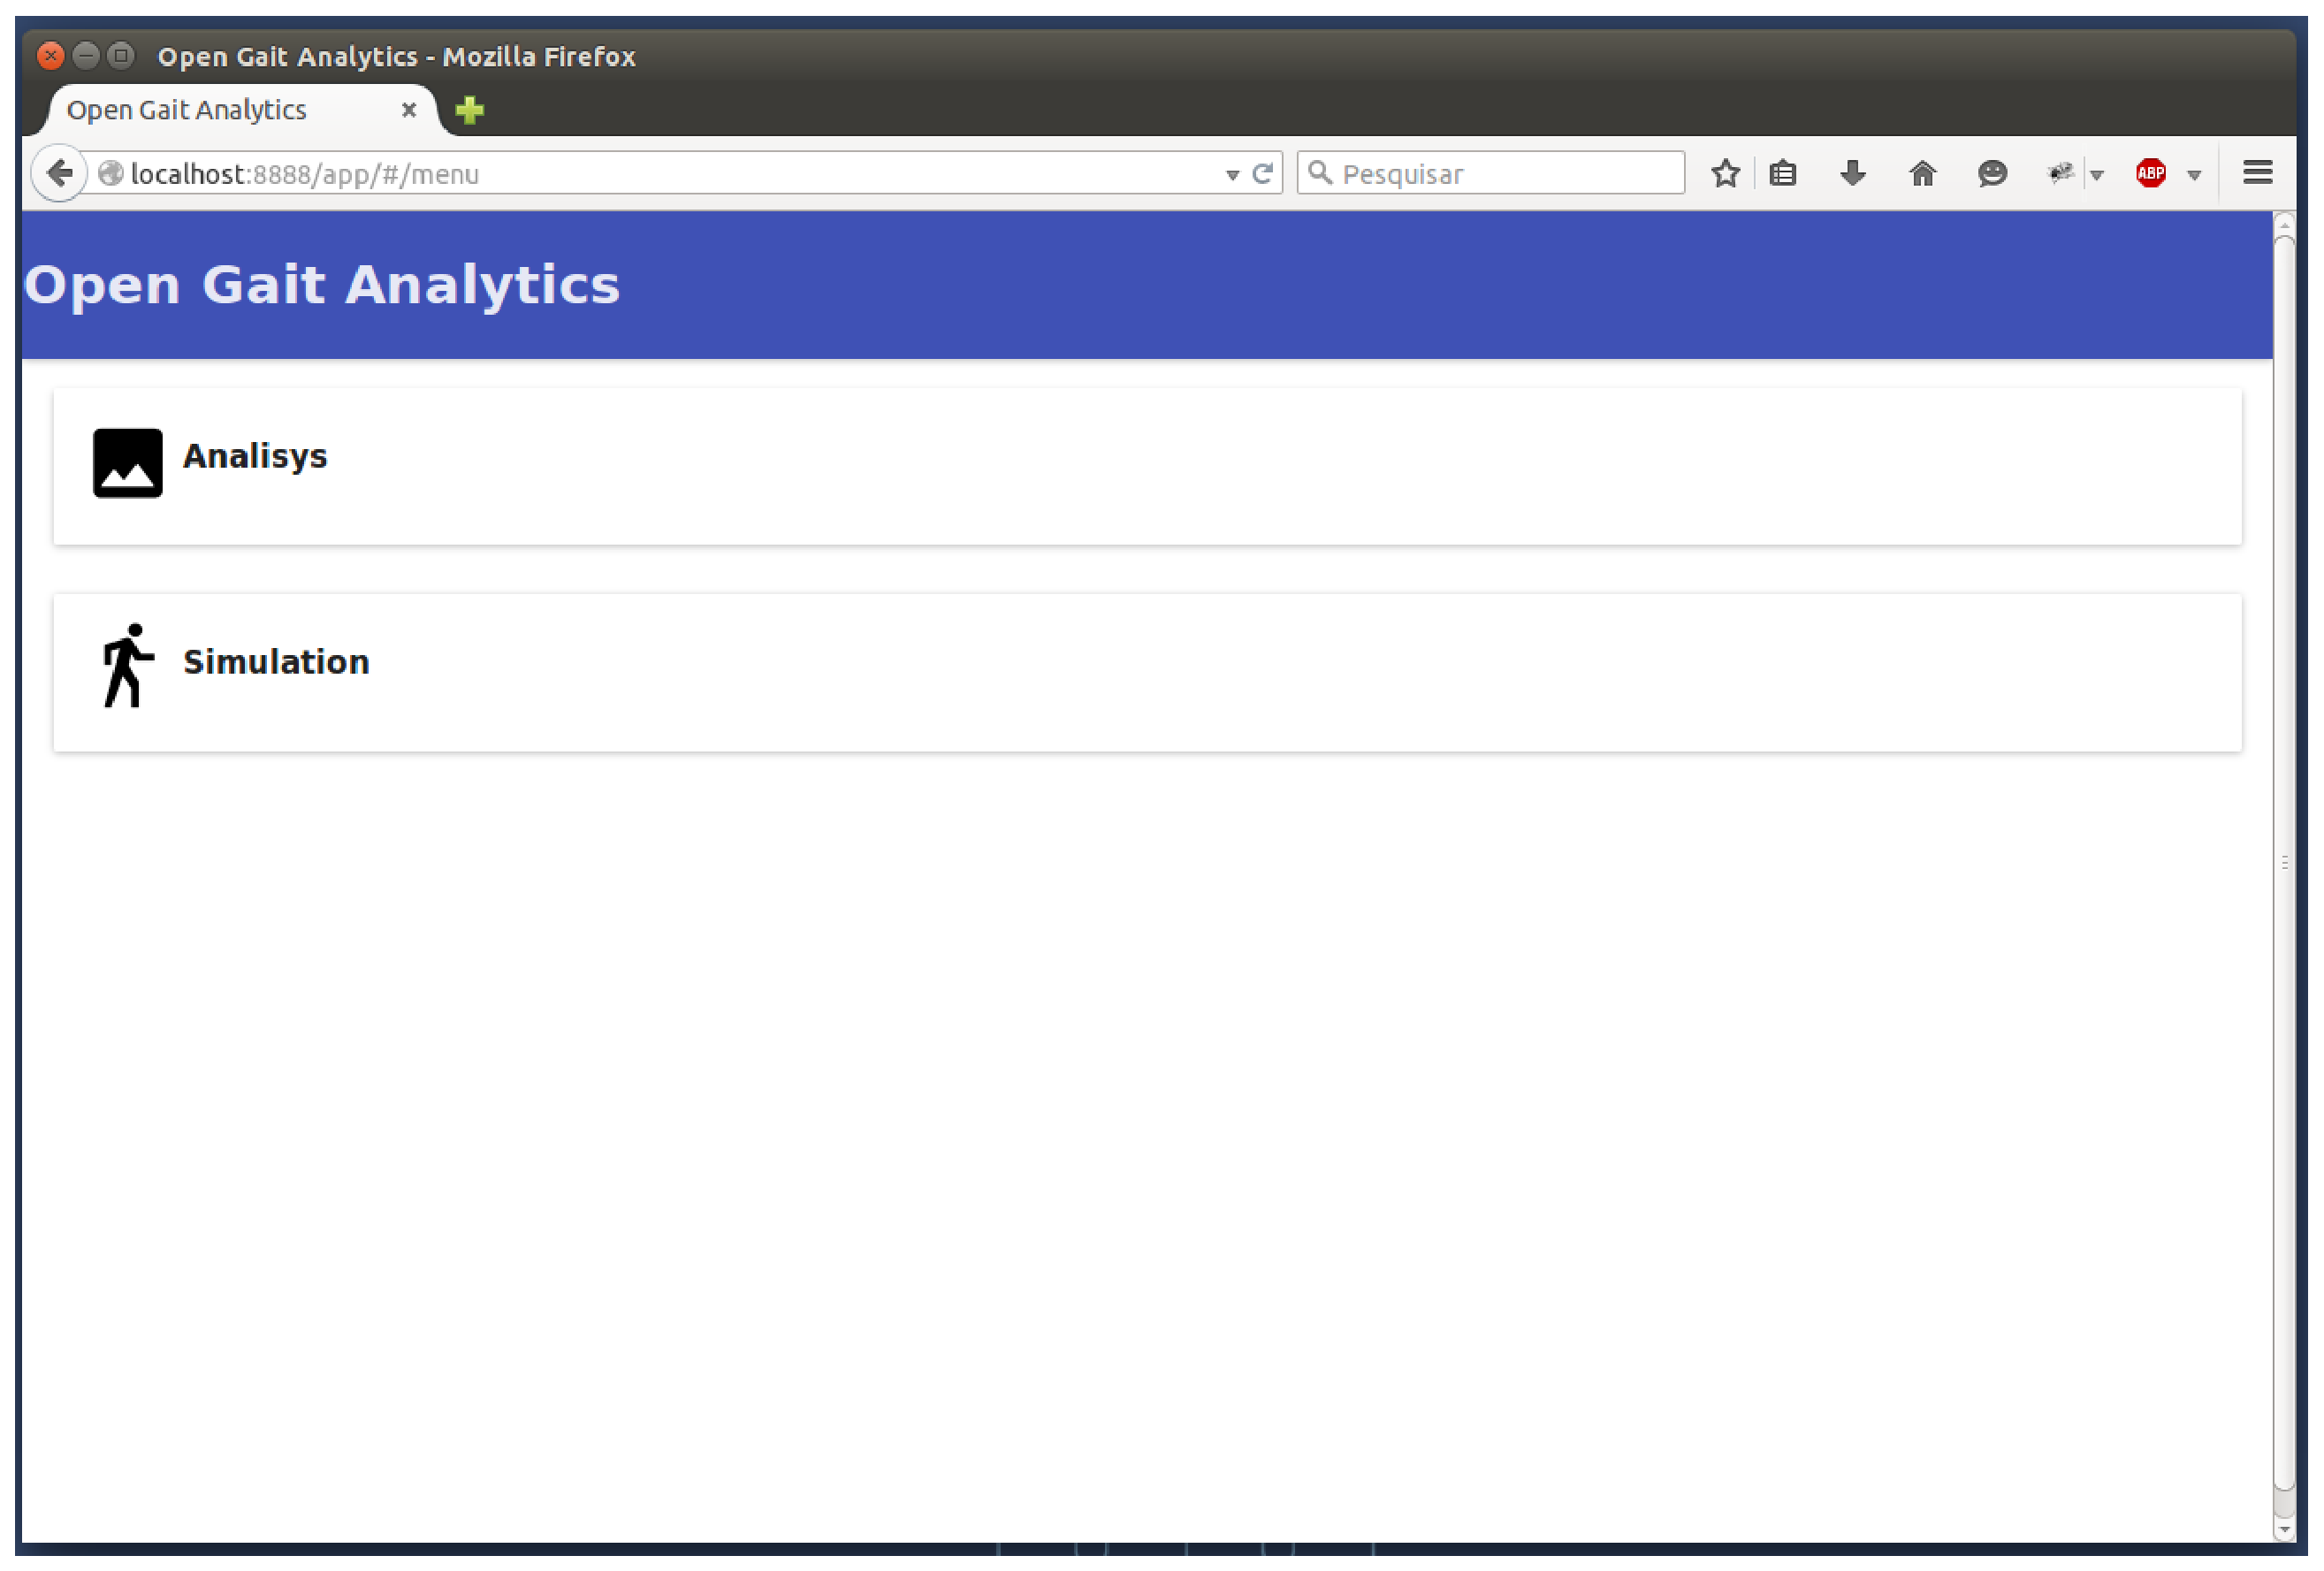
\includegraphics[width=15cm]{figuras/tela1.eps}
	\caption{Tela de seleção dos módulos.}
	\label{tela1}
\end{figure}

\section{Módulo de Análise}
Neste fase o software conta apenas com análise de movimentos, com sinais oriundos de marcadores passivos de superfície, captados por câmeras, usando o software \emph{QTM}. 
No \emph{QTM} é feita a conversão dos dados para o formato \emph{Matlab} que é reconheciodo pelo sistema construído.

A primeira tela deste módulo pode ser vista na Figura \ref{tela2}. Este tela apresenta a listagem de pacientes, cadastrados no sistema. O botão abaixo a direita, é a função para adicionar novos pacientes.

\begin{figure}[ht]
	\centering
	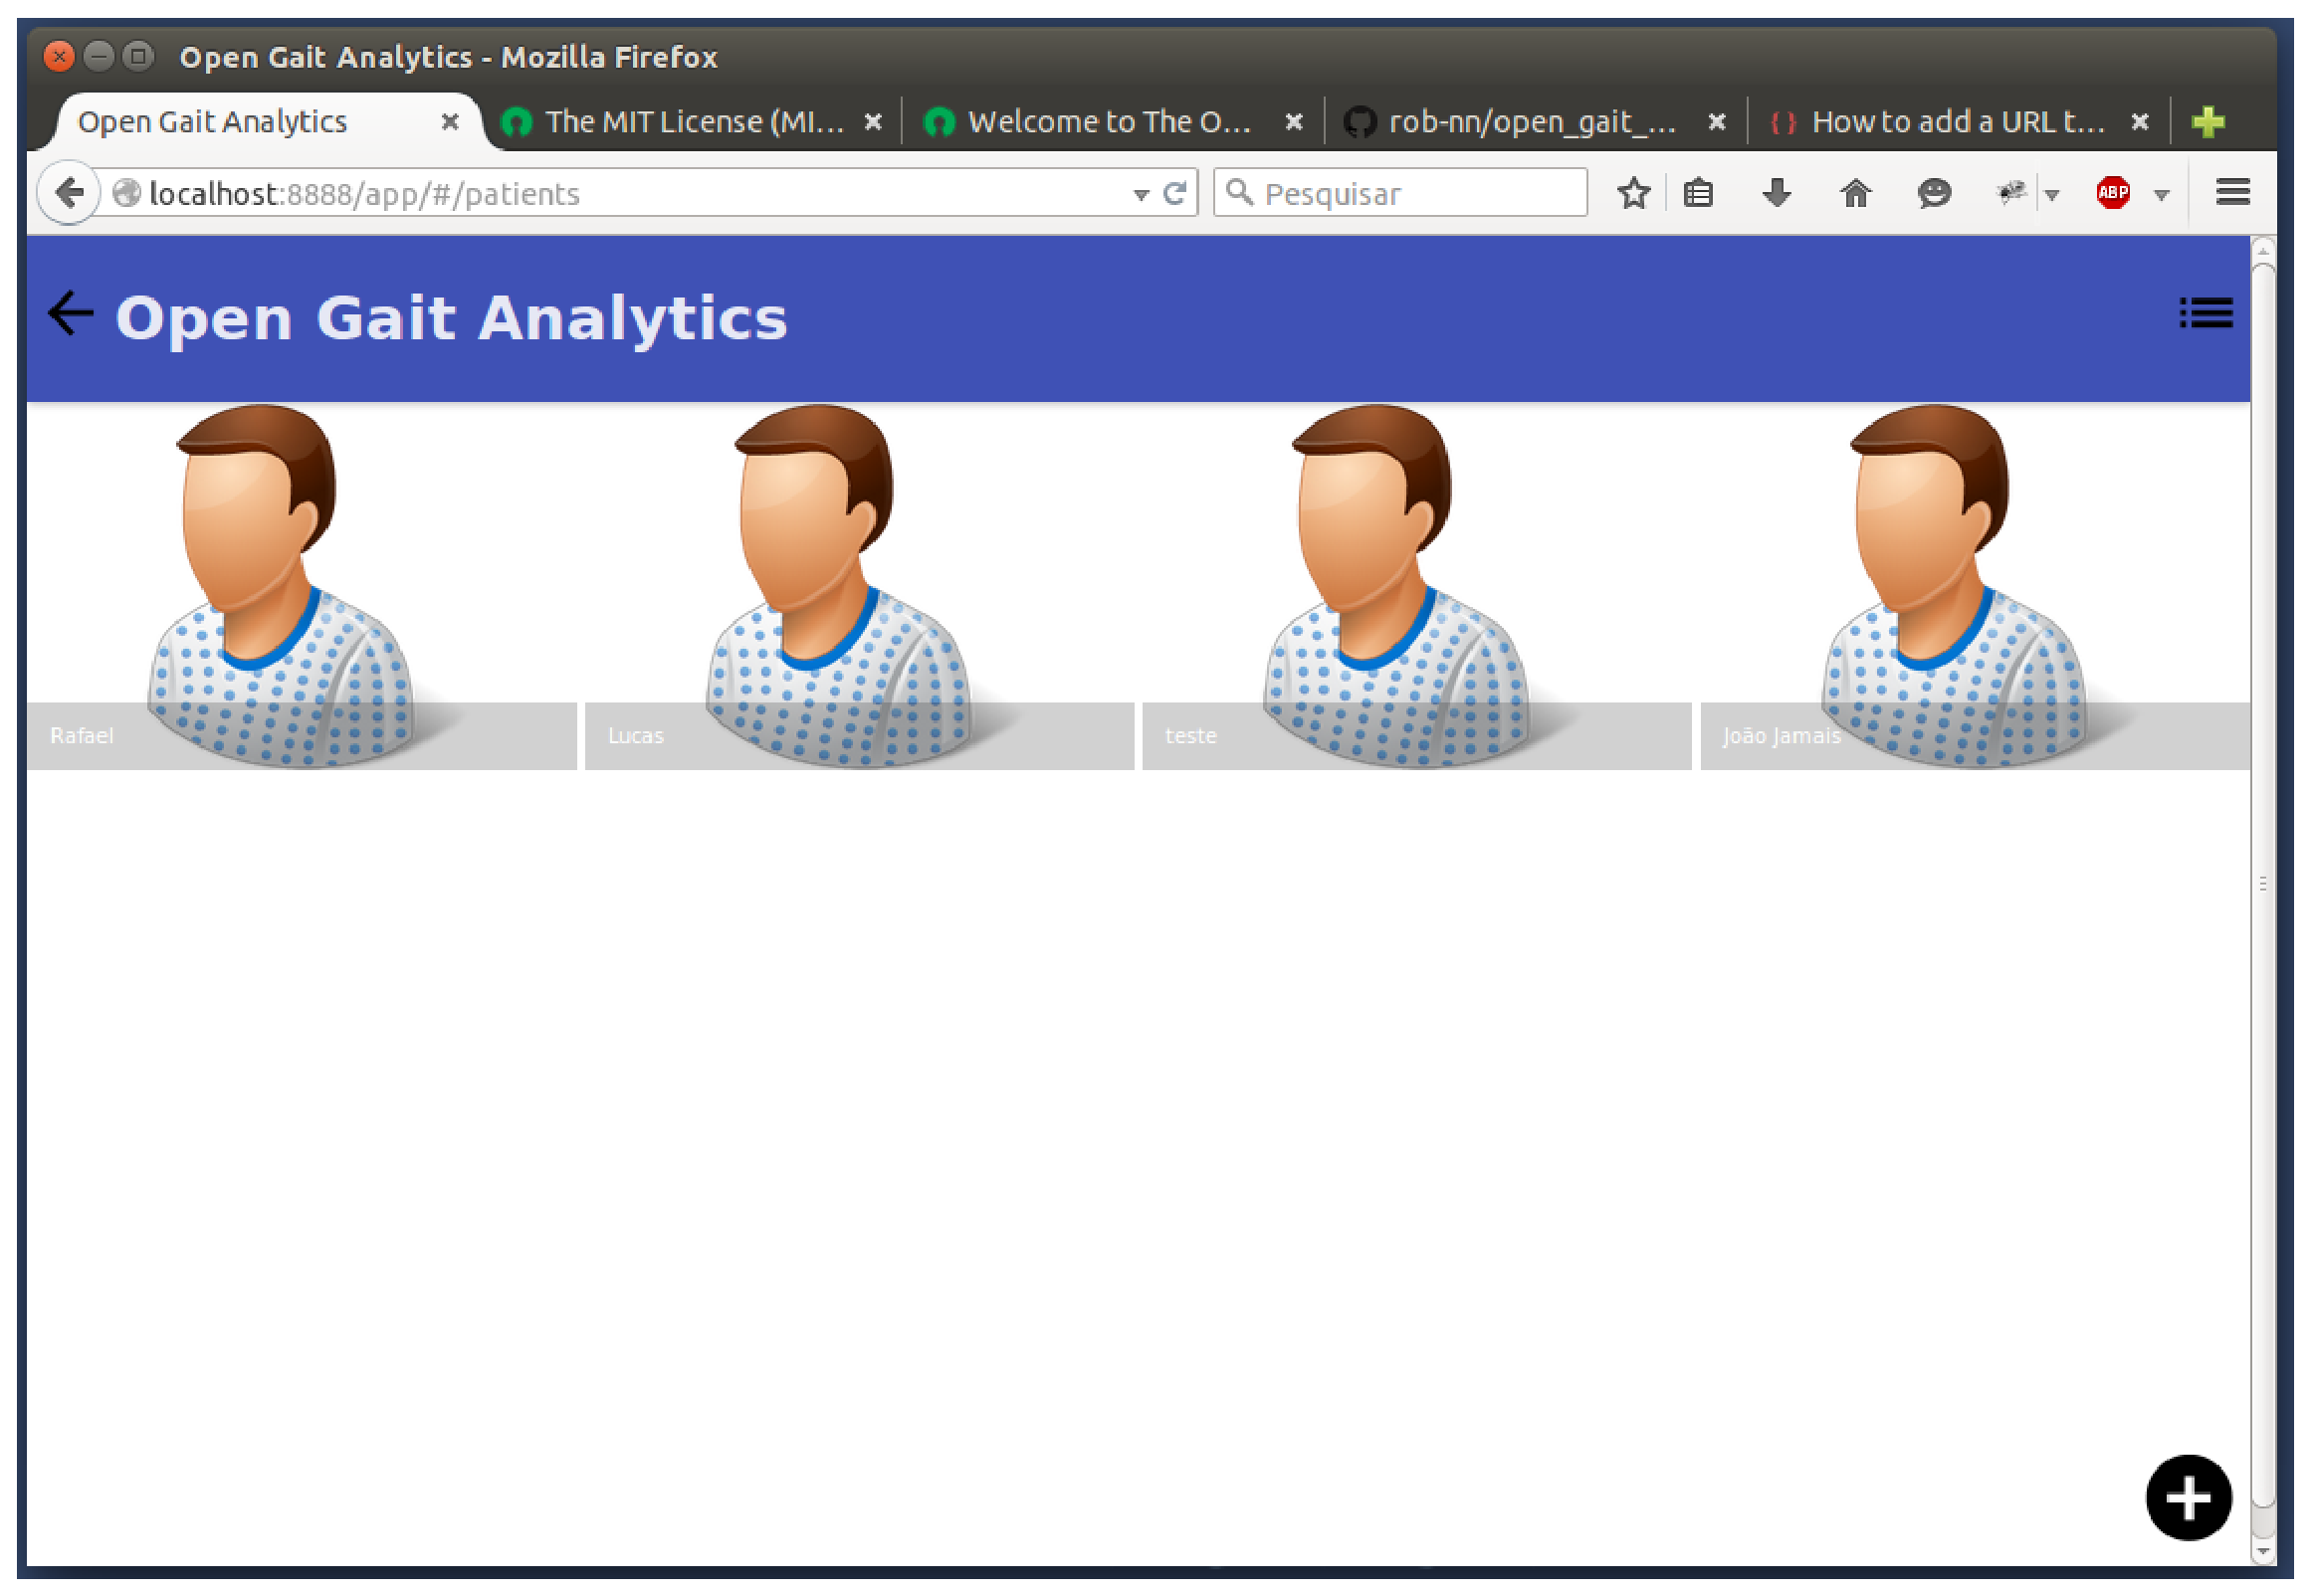
\includegraphics[width=15cm]{figuras/tela2.eps}
	\caption{Tela com a listagem de pacientes.}
	\label{tela2}
\end{figure}

A Figura \ref{tela3} mostra as informações do paciente que devem ser preenchidas ao se executar a função adicionar paciente. Esta tela é uma adaptação da ficha de avaliação que está na obra \citeonline{VeraReg}.

\begin{figure}[ht]
	\centering
	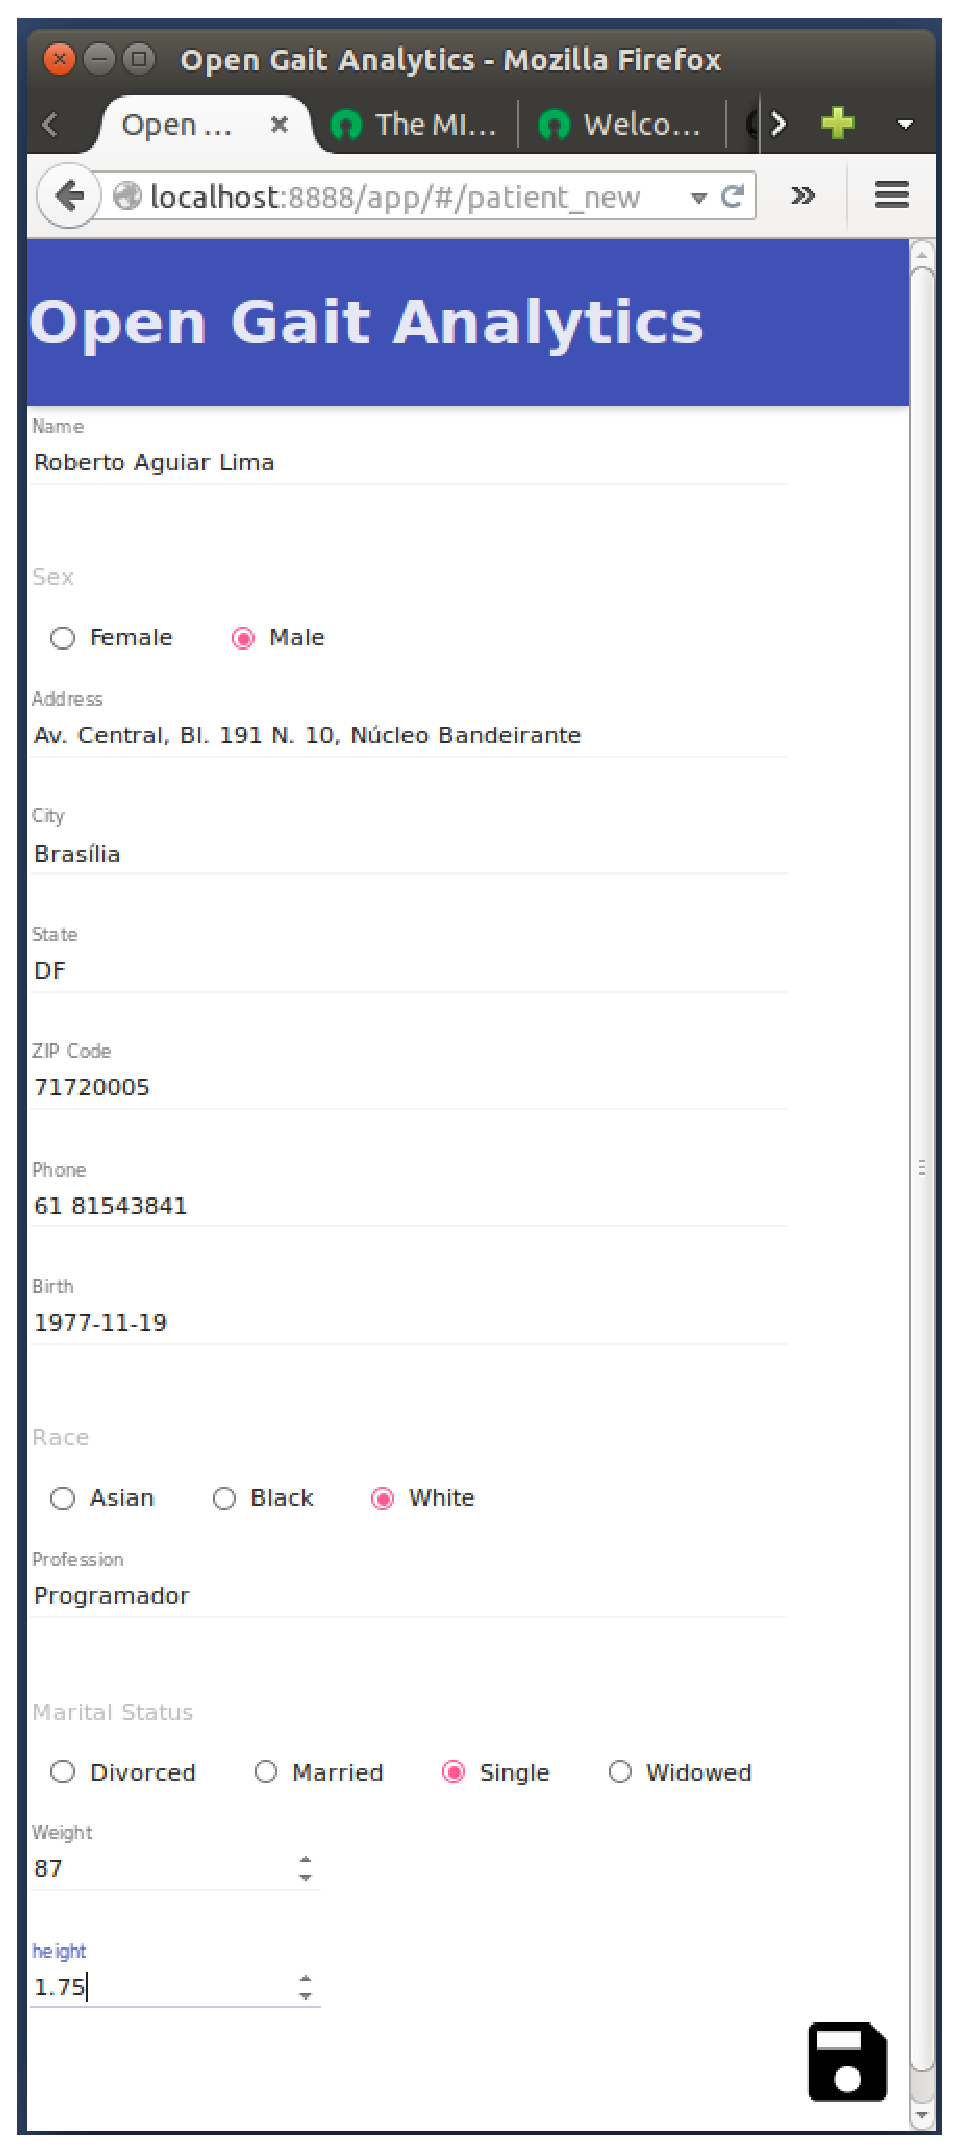
\includegraphics[width=7cm]{figuras/tela3.eps}
	\caption{Informações do paciente.}
	\label{tela3}
\end{figure}

Ao se selecionar um paciente da tela mostrada na Figura \ref{tela2}, a tela da Figura \ref{tela4} aparece. No caso em questão, nenhuma coleta de dados foi carregada para o paciente. Logo o próximo passo é adicionar uma nova amostra de marcha.
O usuário deve então informar a descrição da coleta e a data que a mesma ocorreu e salvar ests informações, conforme a Figura \ref{tela5}.


Depois de salva as informações o sistema pede para que o usuário selecione o arquivo proveniente do \emph{QTM}, conforme a Figura \ref{tela6}.
Depois de selecionado o arquivo com os dados da marcha, seus dados são mostrados para o usuário, conforme a Figura \ref{tela7}.


Neste momento se o usuário quiser visualizar uma animação dos dados, basta clicar na seta negra que aponta para a direita que uma animação será mostra conforme a Figura \ref{animacao1}.
Esta animação foi construída usando a tecnologia \emph{ThreeJS}, resumida na seção \ref{threejs_sec}. Uma das grandes vantagens desta característica do software em relação ao \emph{QTM}, que também a possui, é o fato de que a animação está rodando num \emph{browser web} moderno, ou seja qualquer um com um \emph{browser} assim pode vê-la sem precisar do \emph{QTM} instalado. 
Além do mais como o projeto pode continuar, fica a critério dos usuários decidirem que novas características seriam interessantes, não somente nas animações, mas em todo o software.

A tela da animação também possui controle de pespectivas, ver Figura \ref{animacao2}, controle de \emph{zoom}, ver Figura \ref{animacao3}, e controle \emph{pan}, ver Figura \ref{animacao3}.
Também foram implementados, até o momento, botões de \emph{play, pause}, fechar e um contador de \emph{frames}, ver Figura \emph{animacao4a}.




É de fundamental importância que o usuário configure os parâmetros \emph{Initial Contact} e \emph{Terminal Swing} mostrados na Figura \ref{tela7}. Sem estes parâmetros os gráficos, vão mostrar os sinais nas fases erradas do ciclo de marcha.
A técnica que se recomenda, é inicializar a animação e quando o usuário perceber o \emph{initial contact}, pressionar o botão pause e anotar o frame. Fazer a mesma coisa para o \emph{terminal swing}.

Outra opção disponível na Figura \ref{tela7}, é a opção \emph{Markers}, esta opção permite nomear os marcadorese visualizar sua progressão espacial. A Figura \ref{tela18} mostra o resultado de se selecionar esta opção.
Ao clicar no botão ao lado de algum marcador, sua progressão no espaço é mostrada num gráfico como o da Figura \ref{tela19}. O domínio é o percentual do ciclo de marcha, já a imagem são dados espaciais brutos oriundos do \emph{QTM}.

A nomeação dos marcadores, não é uma tarefa trivial. Para isso foi criada uma ferramenta dentro da animação para ajudar com esta tarefa. Primeiro deve-se entrar na animação, depois pausá-la, e posicionar a visualização de uma forma que ajude a detectar o marcador procurado. Veja a figura \ref{tela20}, nela um marcador foi clicado com o \emph{mouse}, o marcador ficou azul e ao seu lado ele mostra o índice 30. 
Agora é só voltar na opção de marcadores, procurar o índice 30 (\emph{Marker 30}) e colocar o nome desejado. No caso deste marcador o nome é joelho esquerdo (\emph{left knee}), ver a Figura \ref{tela21}.
Agora para o sistema o marcador 30 é sempre o joelho esquerdo, veja a Figura \ref{tela22}.

Outra funcionalidade importante é o gerador de ângulos. Esta opção está disponível da Figura \ref{tela7}. E após selecionada é mostrada na Figura \ref{tela23}. 
Para se gerar um ângulo o usuário necessita selecionar a opção de inclusão de ângulo e preencher os dados da Figura \ref{tela24}. O usuário precisa indicar a origem do ângulo, por exemplo o joelho, o componente A, por exemplo algum músculo da coxa, e o componente b, por exemplo a tíbia. Estes pontos poderial representar o ângulo de um joelho por exemplo.

Depois dos ângulos criados é possível ver seus valores durante o ciclo de marcha ou suas velocidades angulares, veja a Figura \ref{tela25} e a Figura \ref{tela26}.

\begin{figure}[ht]
	\centering
	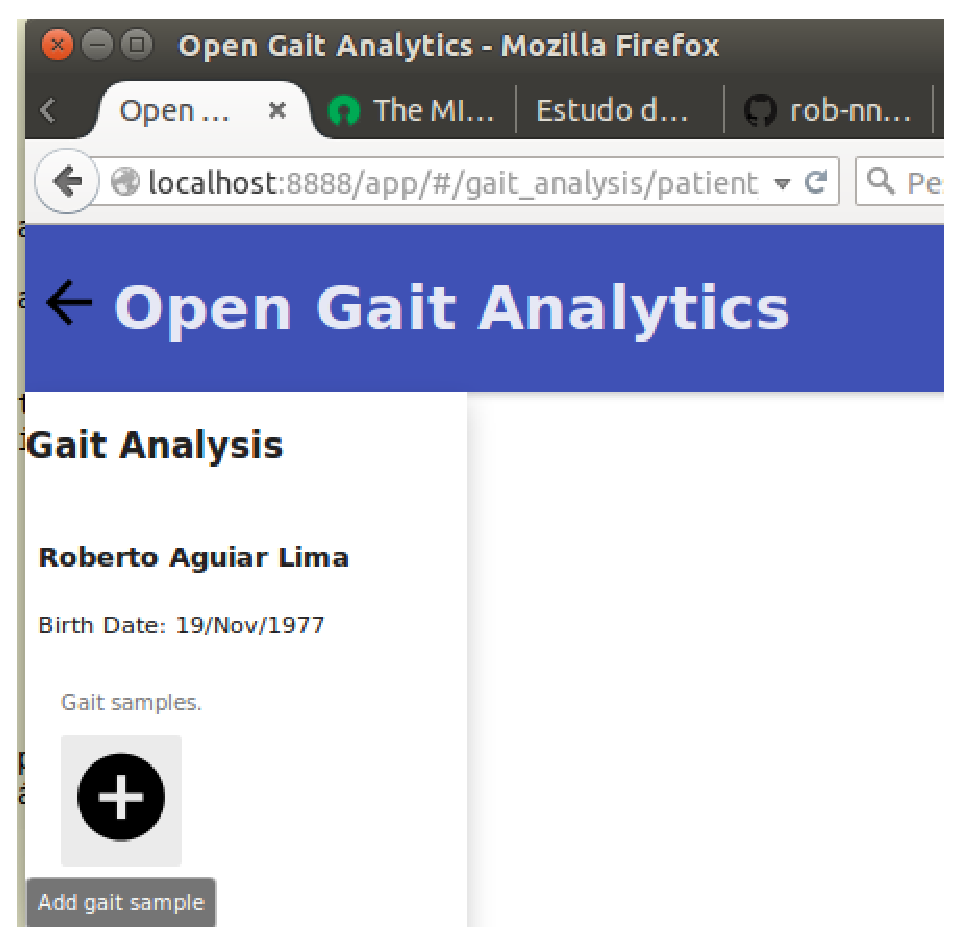
\includegraphics[width=7cm]{figuras/tela4.eps}
	\caption{Tela inicial da dados coletados do paciente.}
	\label{tela4}
\end{figure}


\begin{figure}[ht]
	\centering
	\includegraphics[width=15cm]{figuras/tela5.eps}
	\caption{Inclusão de amostra de marcha}

	\label{tela5}
\end{figure}


\begin{figure}[ht]
	\centering
	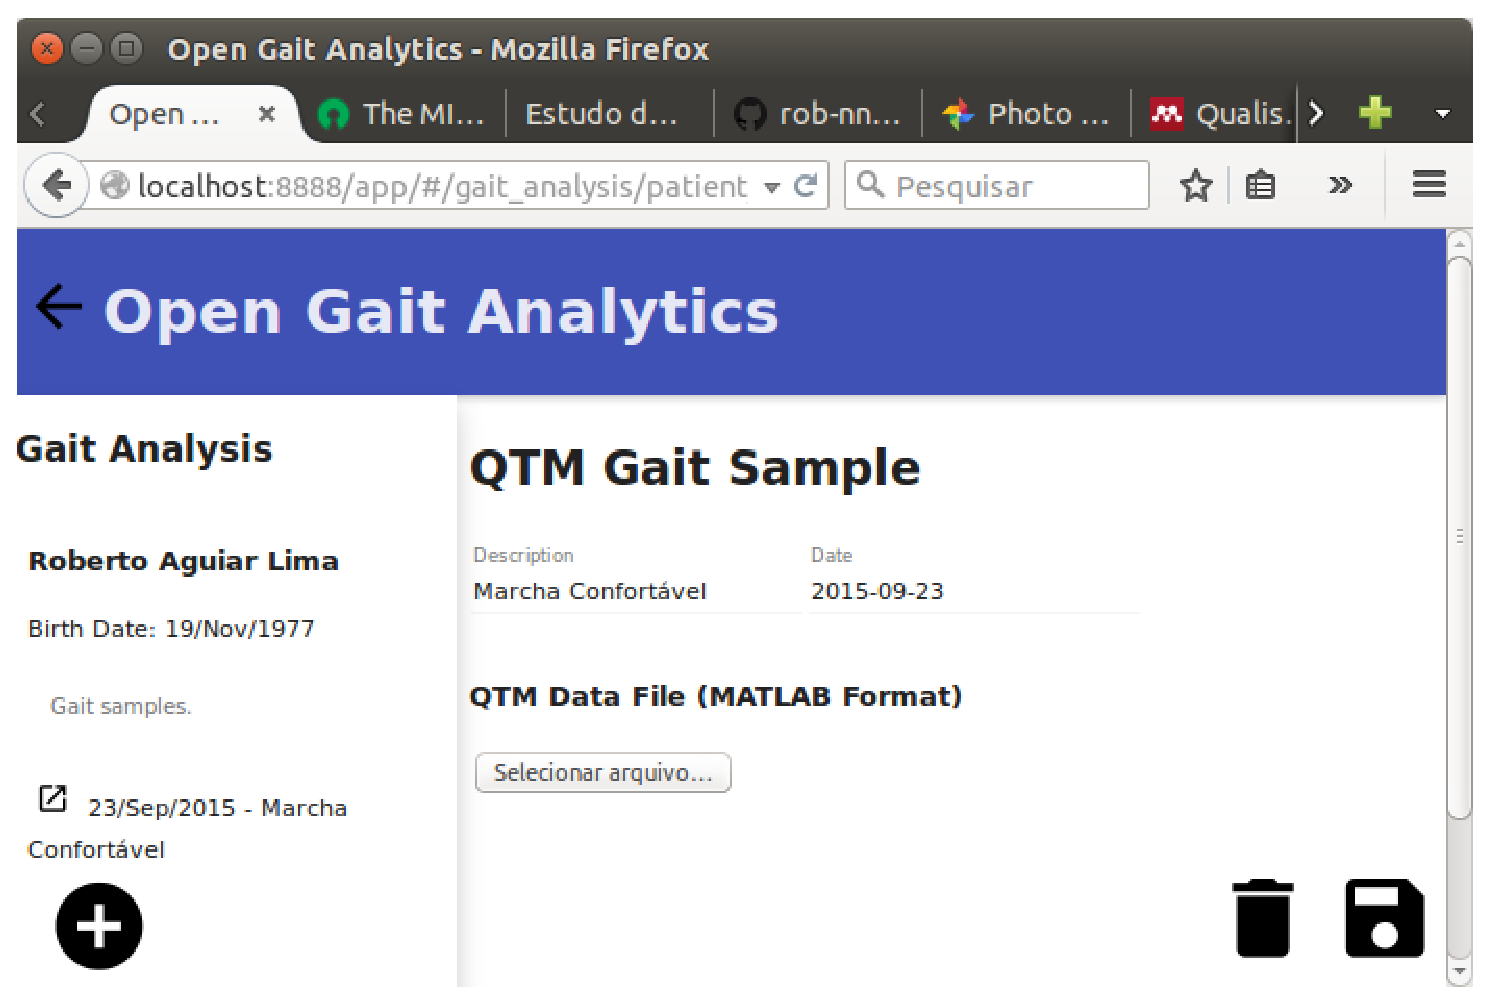
\includegraphics[width=15cm]{figuras/tela6.eps}
	\caption{Seleção do arquivo no formato \emph{MATLAB} proveniente do \emph{QTM}.}
	\label{tela6}
\end{figure}


\begin{figure}[ht]
	\centering
	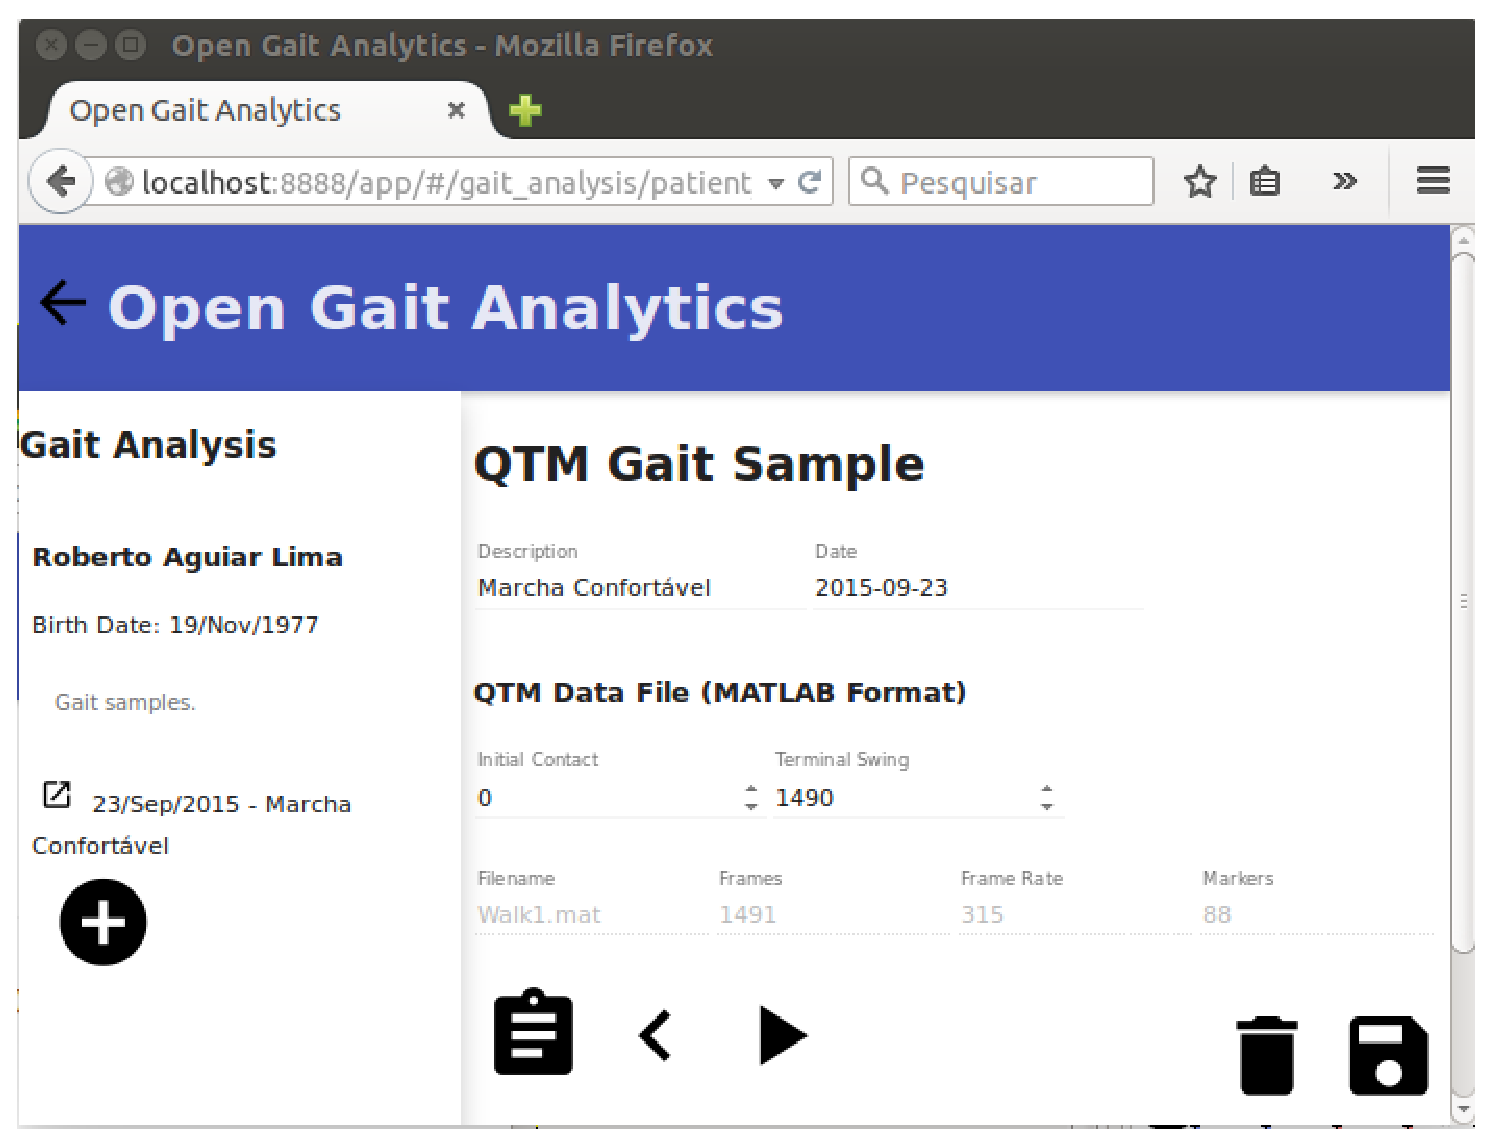
\includegraphics[width=15cm]{figuras/tela7.eps}
	\caption{Dados do arquivo provenientes do \emph{QTM}}.
	\label{tela7}
\end{figure}



\begin{figure}[ht]
  \centering
  \begin{minipage}[b]{0.32\textwidth}
    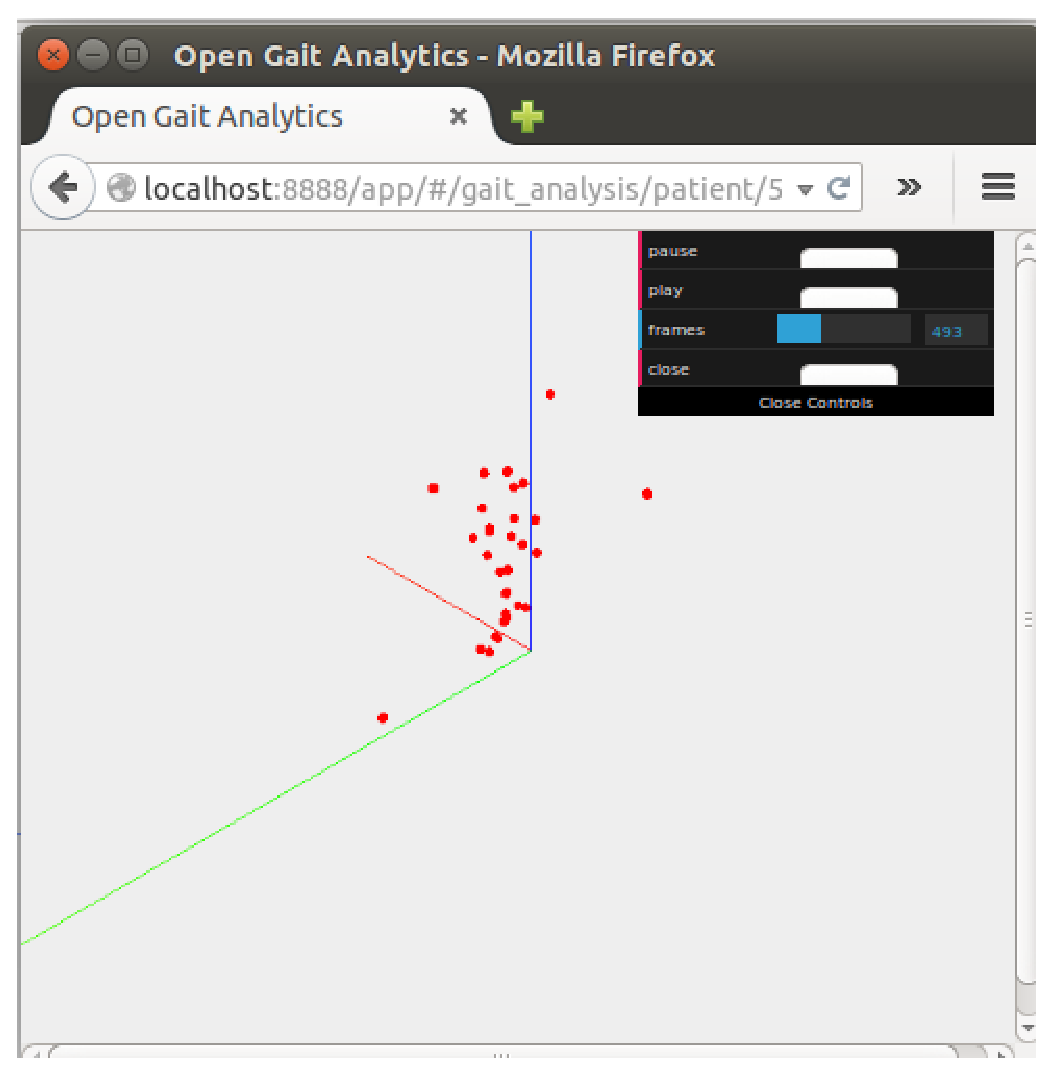
\includegraphics[width=\textwidth]{figuras/tela8.eps}
  \end{minipage}
  \hfill
  \begin{minipage}[b]{0.32\textwidth}
    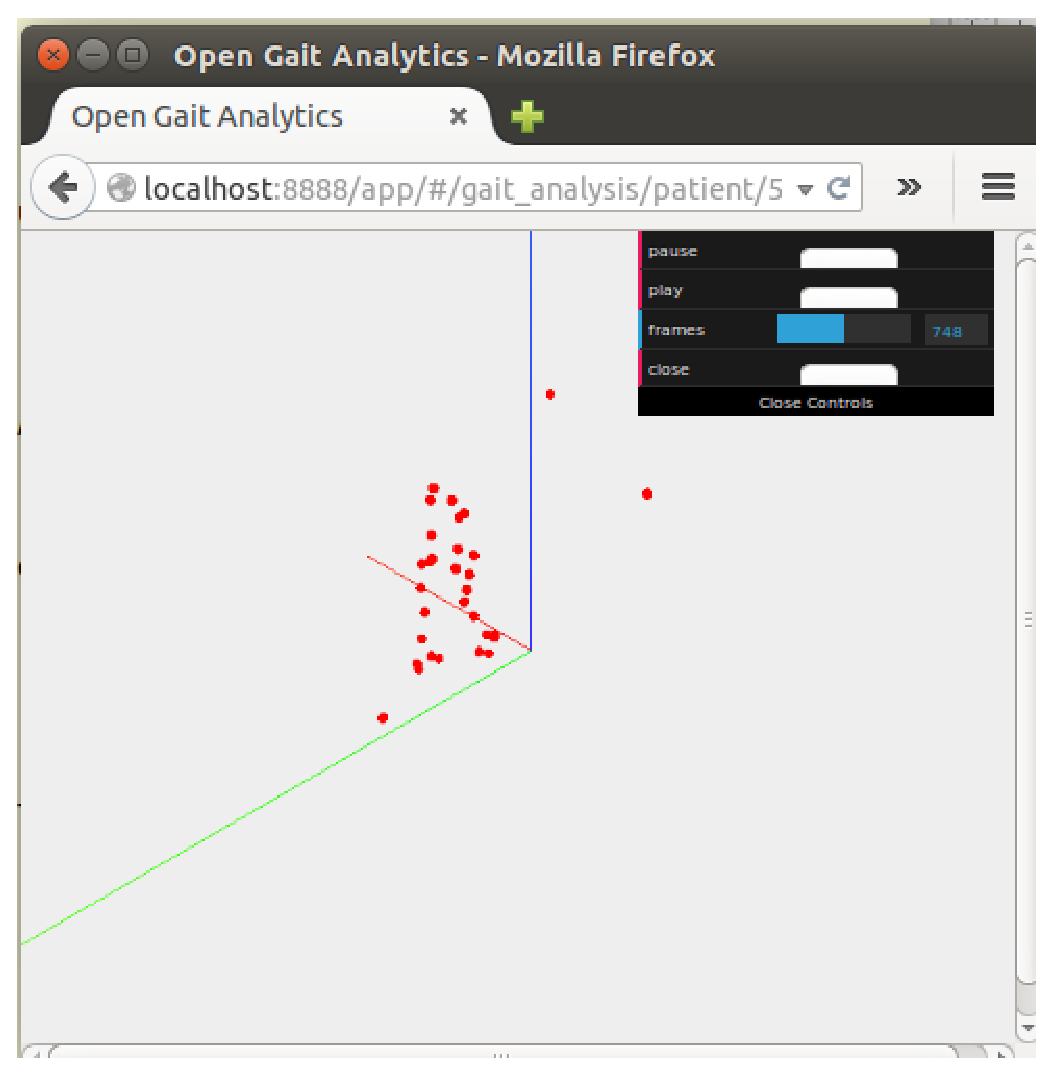
\includegraphics[width=\textwidth]{figuras/tela9.eps}
  \end{minipage}
  \hfill
  \begin{minipage}[b]{0.32\textwidth}
    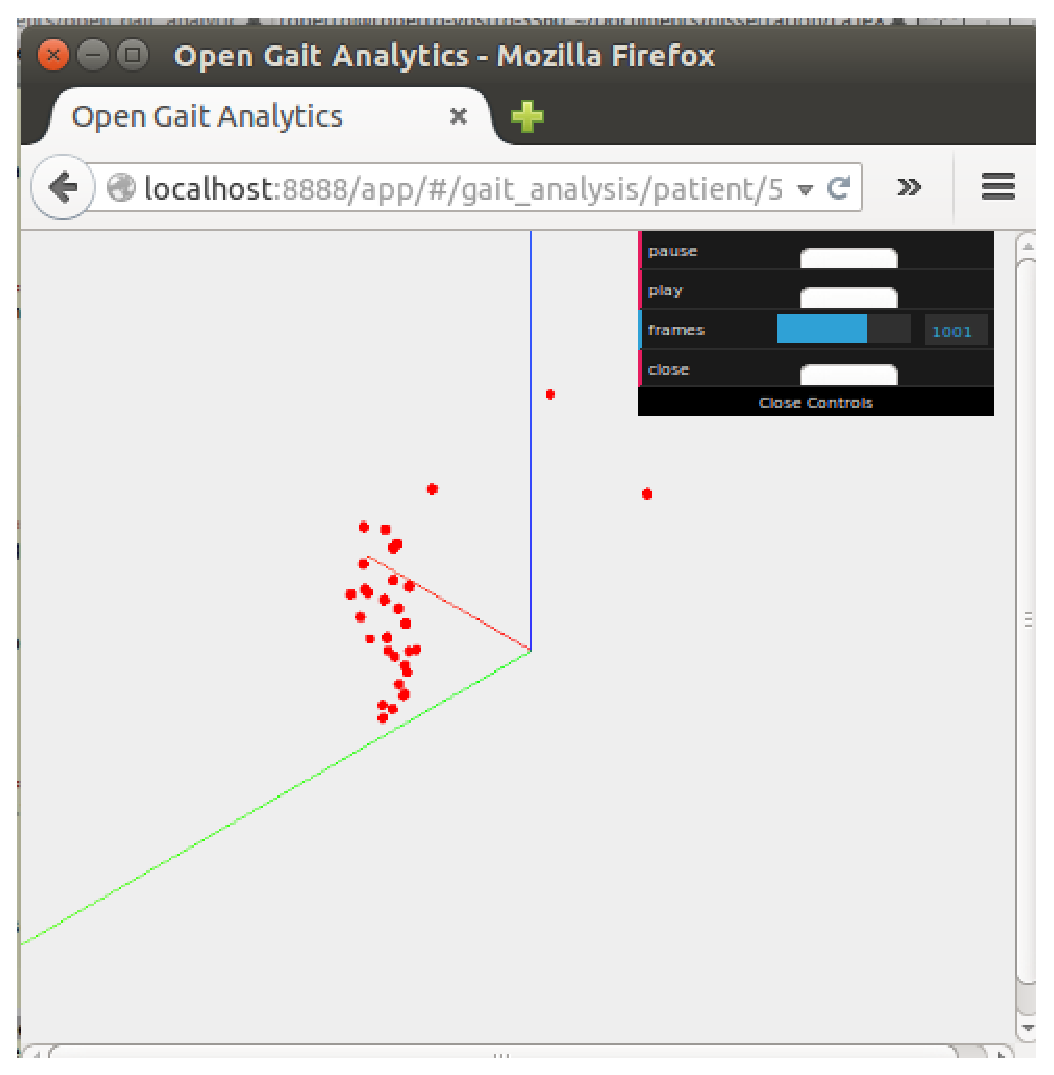
\includegraphics[width=\textwidth]{figuras/tela10.eps}
  \end{minipage}
  \caption{Animação dos marcadores em 3D.}
  \label{animacao1}
\end{figure}


\begin{figure}[ht]
  \centering
  \begin{minipage}[b]{0.49\textwidth}
    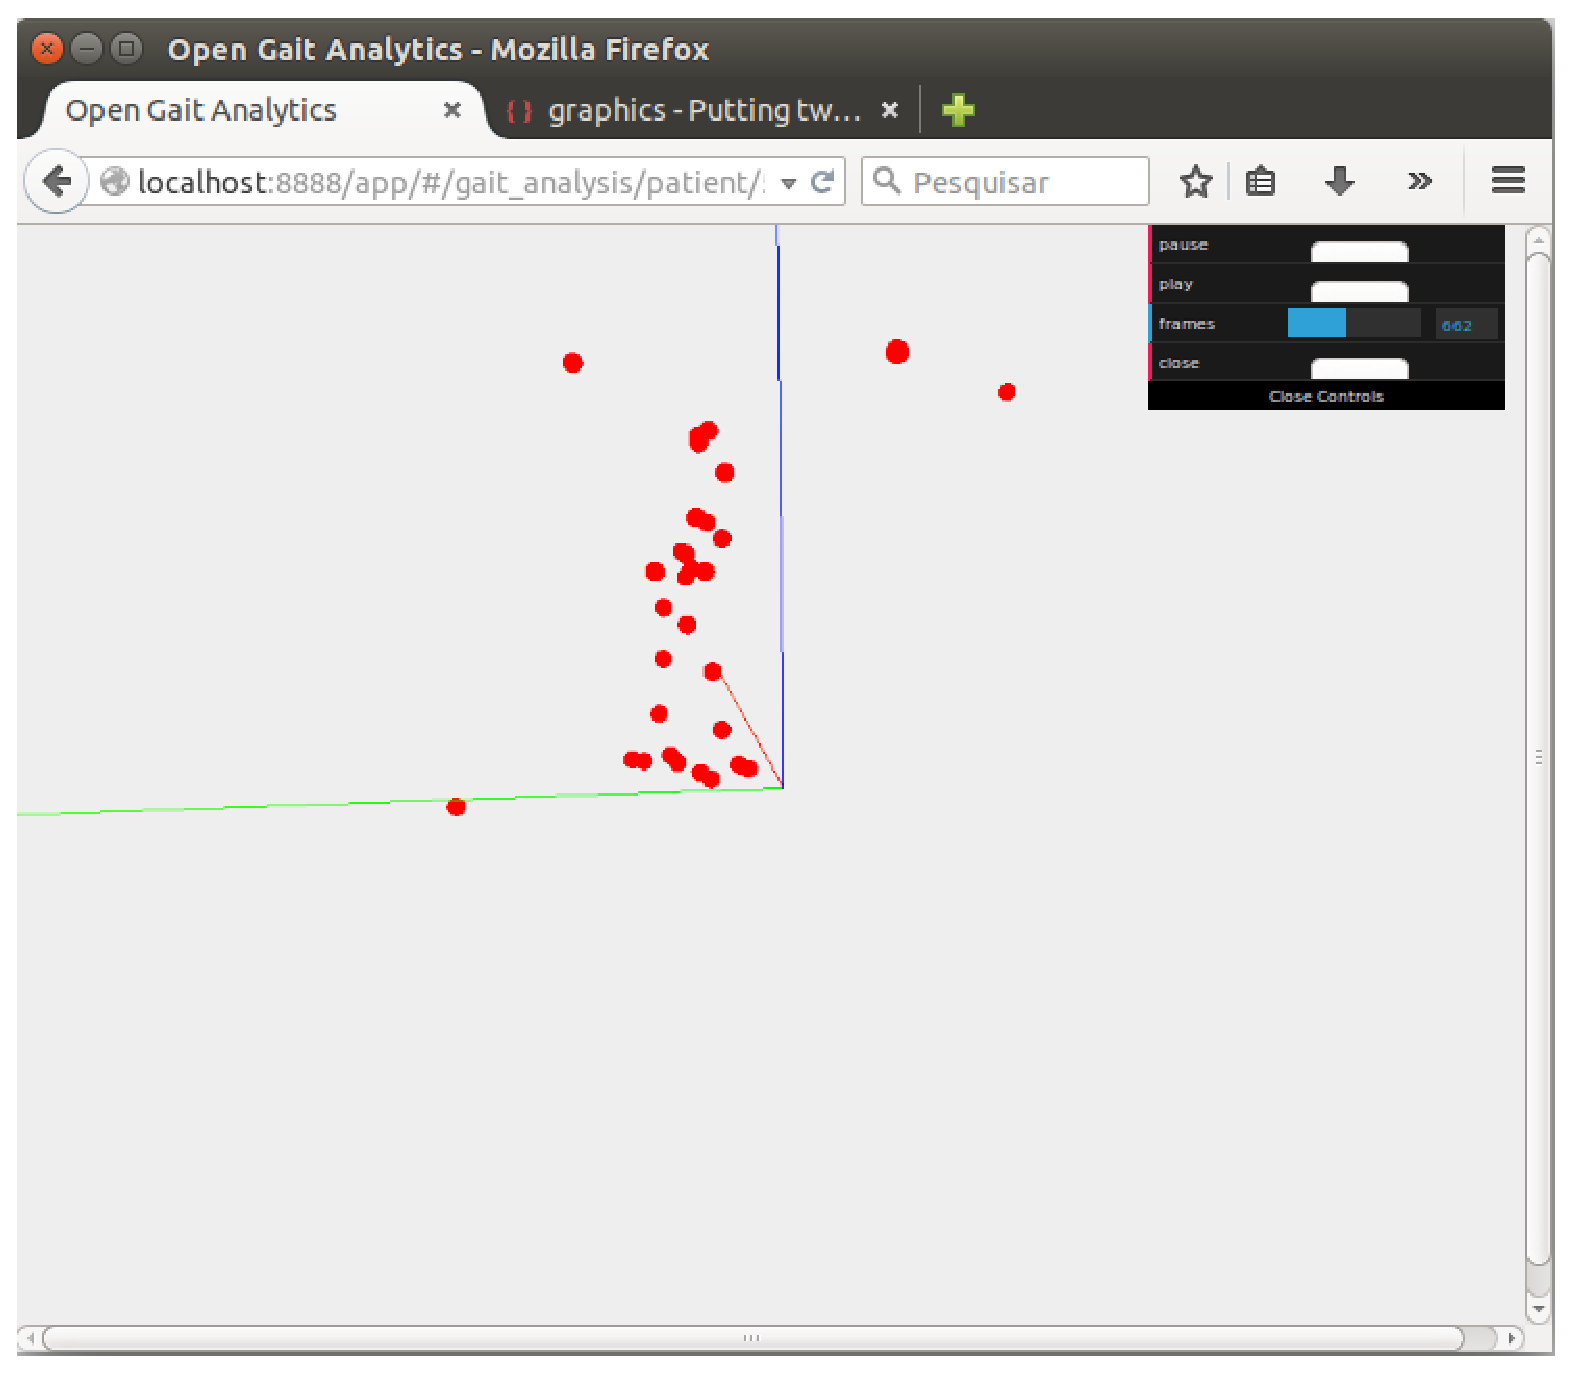
\includegraphics[width=\textwidth]{figuras/tela11.eps}
  \end{minipage}
  \hfill
  \begin{minipage}[b]{0.49\textwidth}
    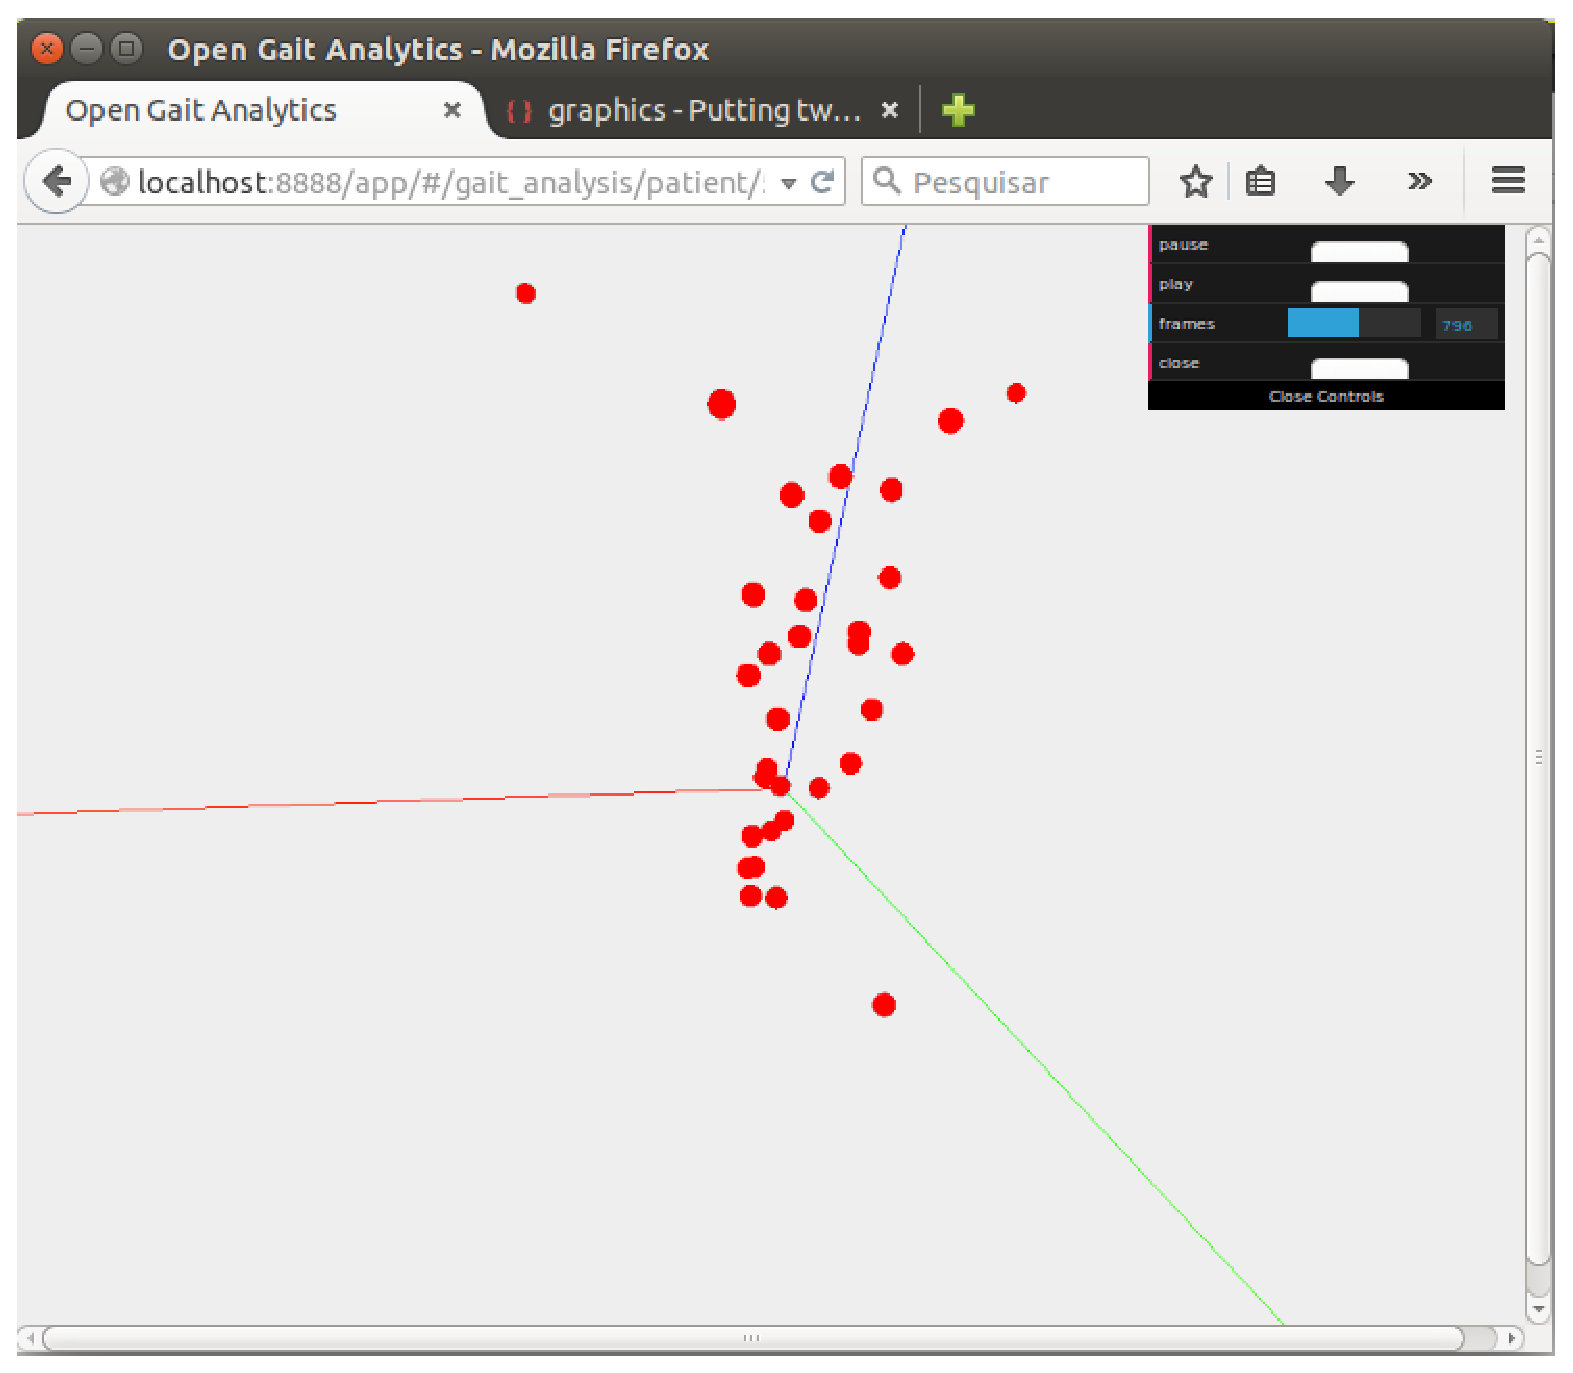
\includegraphics[width=\textwidth]{figuras/tela12.eps}
  \end{minipage}
  \caption{Controle de perspectivas.}
  \label{animacao2}
\end{figure}

\begin{figure}[ht]
  \centering
  \begin{minipage}[b]{0.49\textwidth}
    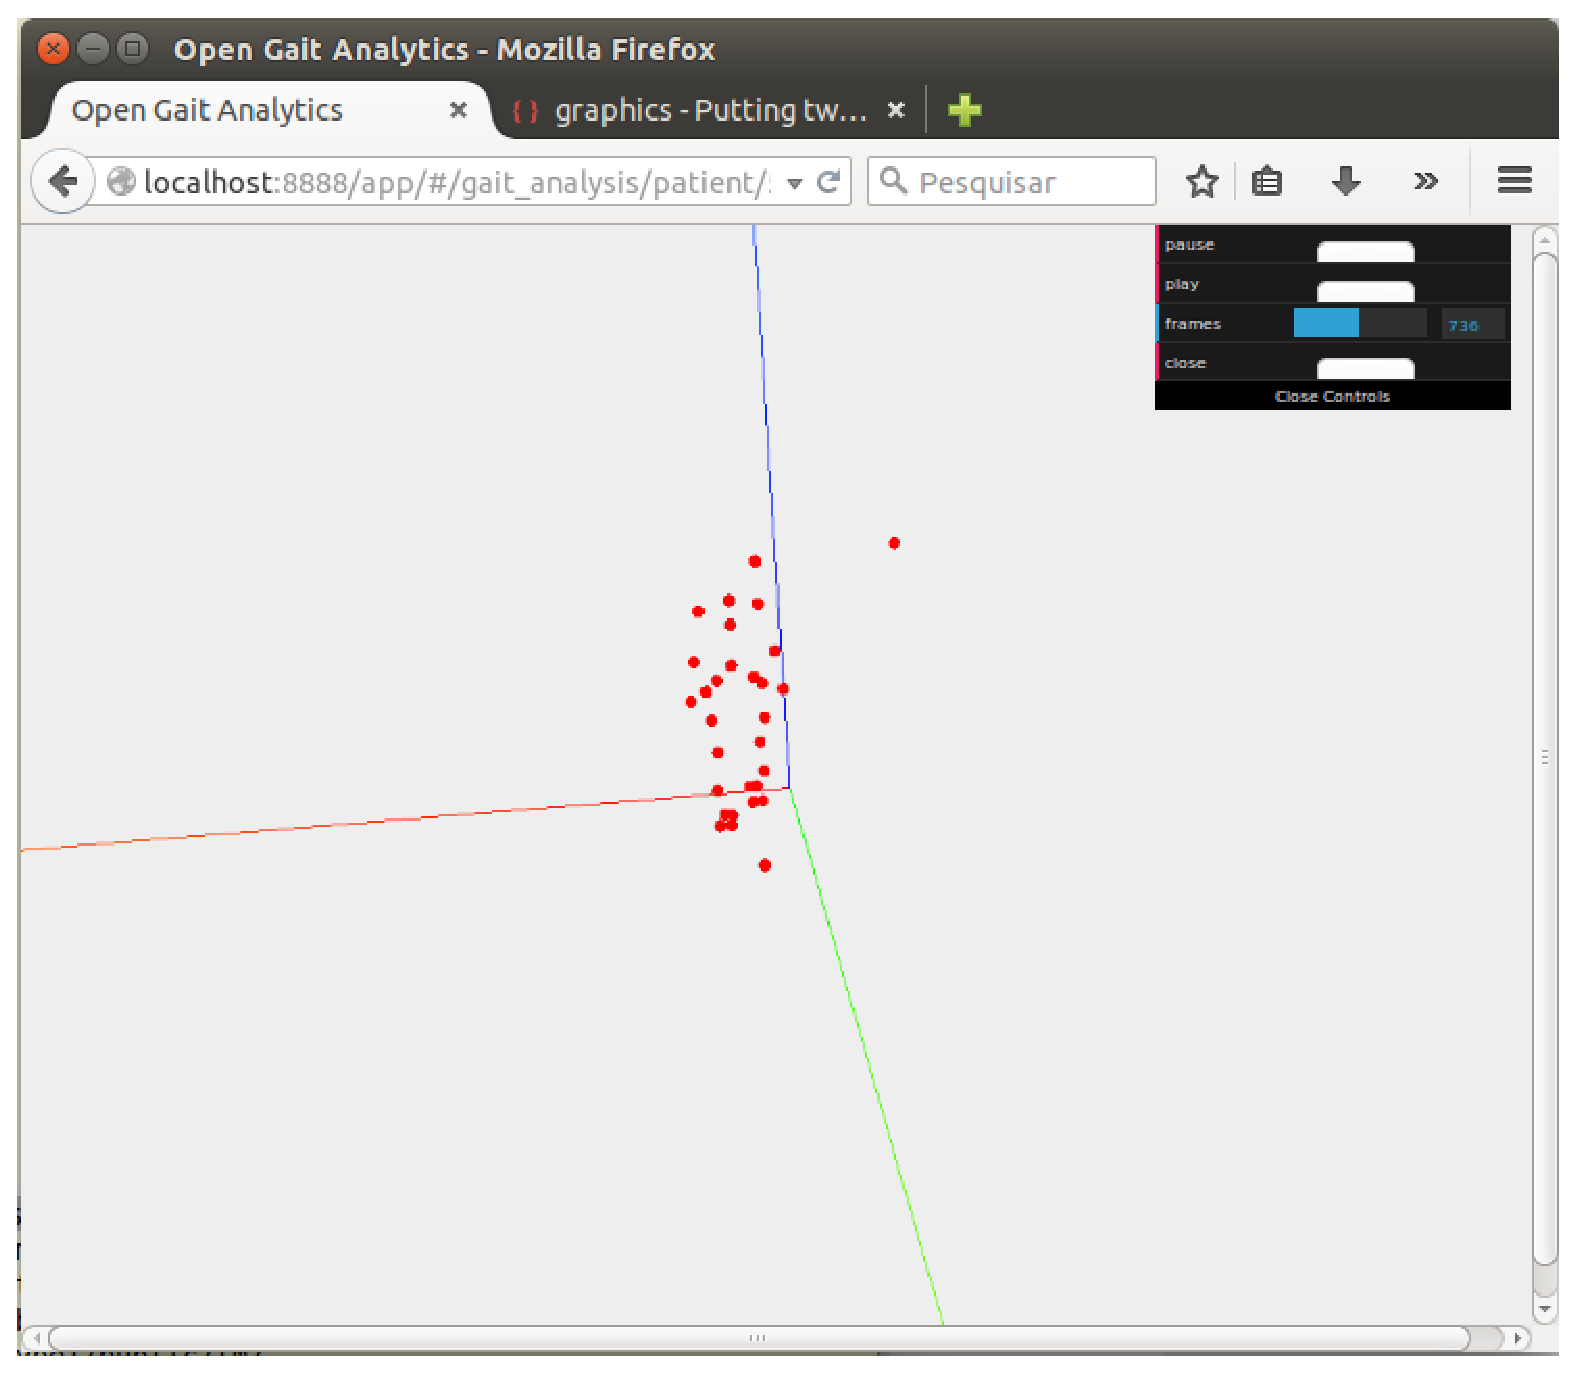
\includegraphics[width=\textwidth]{figuras/tela13.eps}
  \end{minipage}
  \hfill
  \begin{minipage}[b]{0.49\textwidth}
    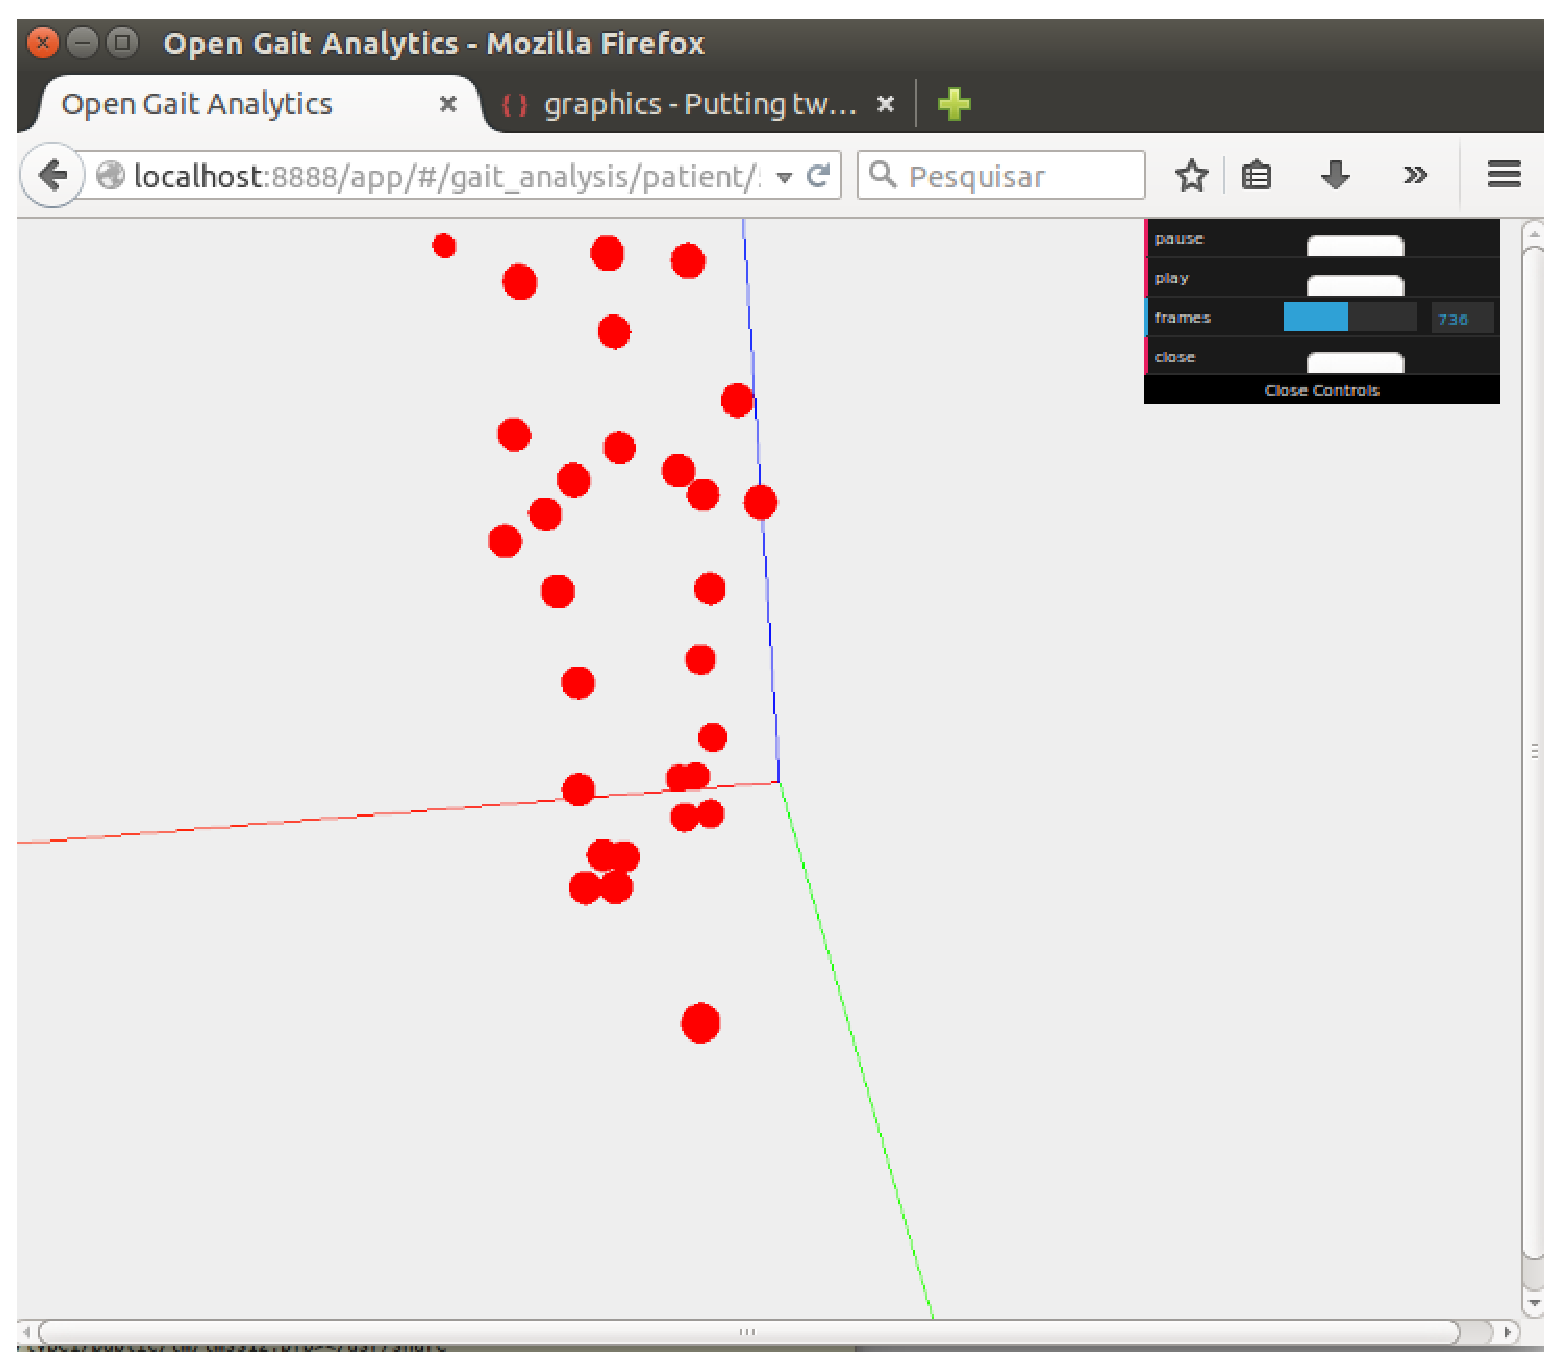
\includegraphics[width=\textwidth]{figuras/tela14.eps}
  \end{minipage}
  \caption{Controle de \emph{zoom}.}
  \label{animacao3}
\end{figure}

\begin{figure}[ht]
  \centering
  \begin{minipage}[b]{0.49\textwidth}
    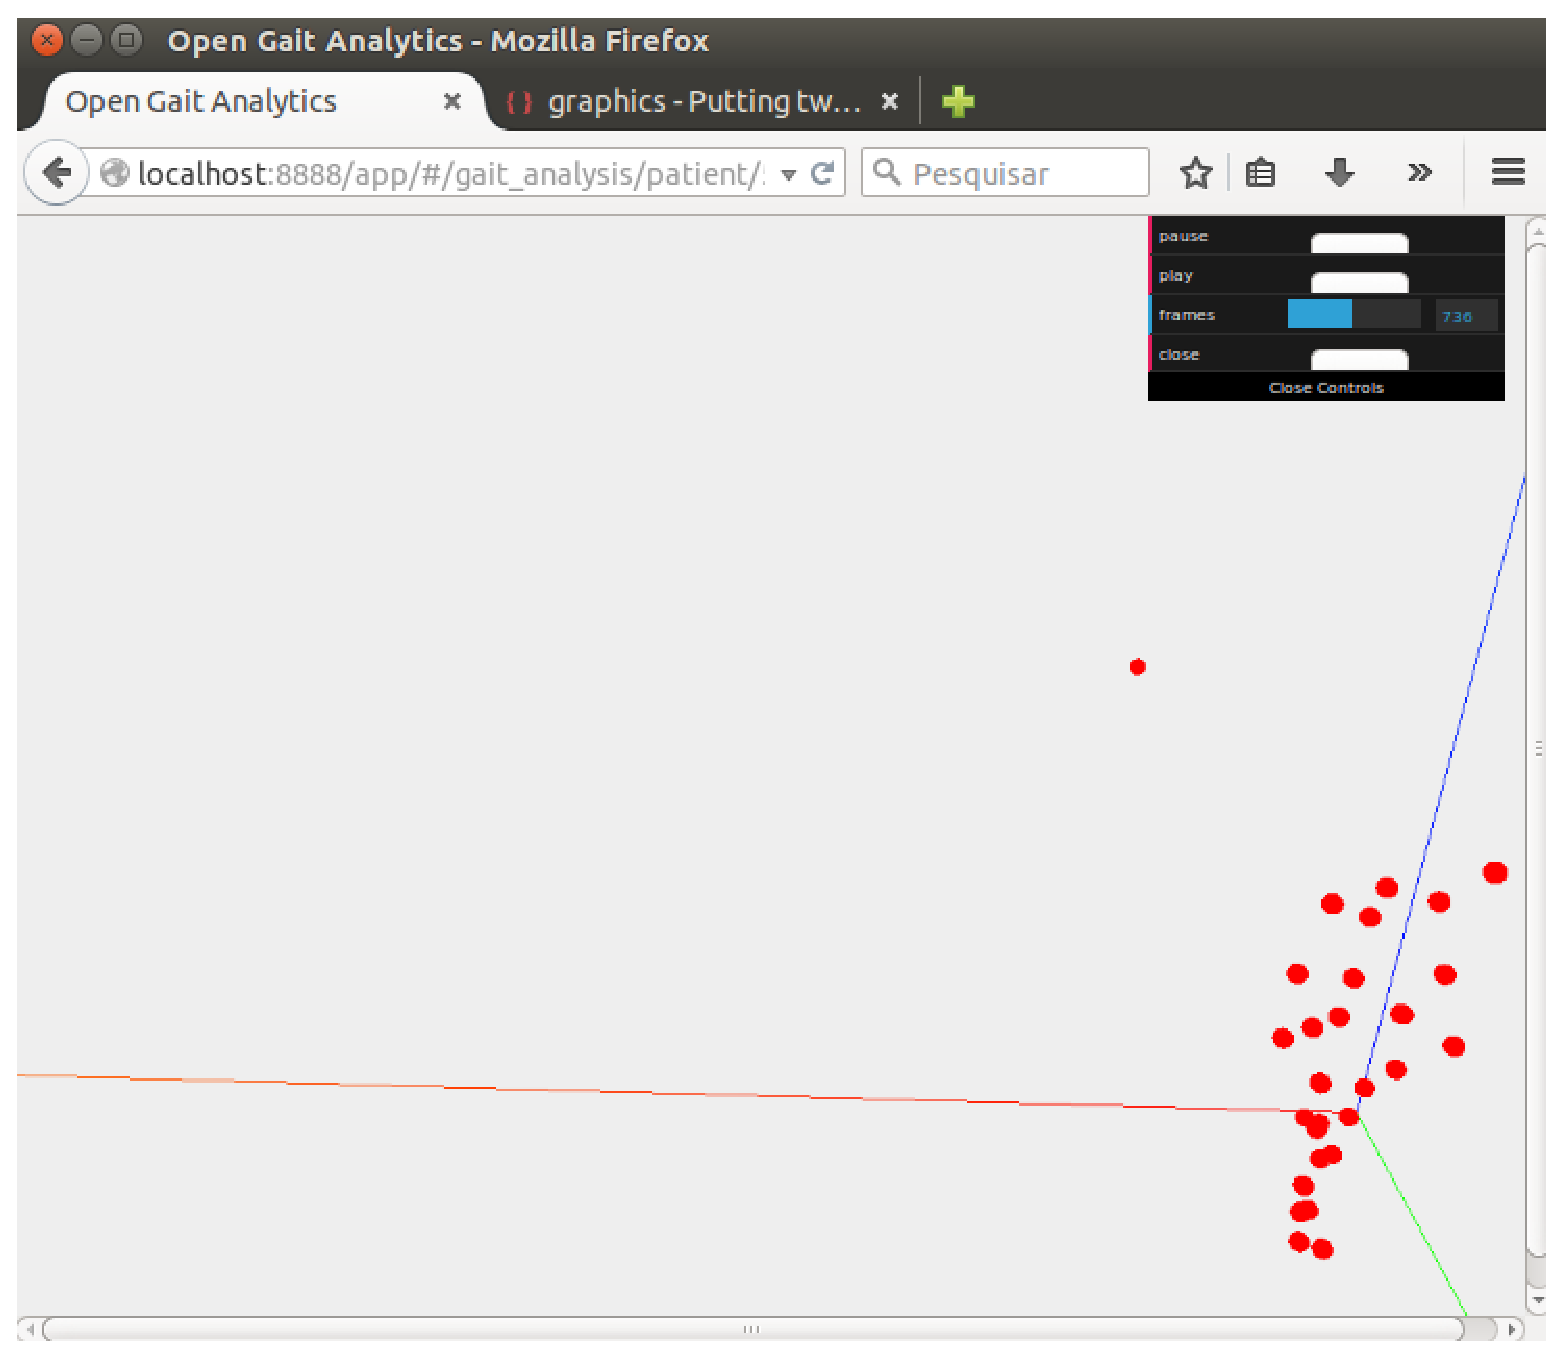
\includegraphics[width=\textwidth]{figuras/tela15.eps}
  \end{minipage}
  \hfill
  \begin{minipage}[b]{0.49\textwidth}
    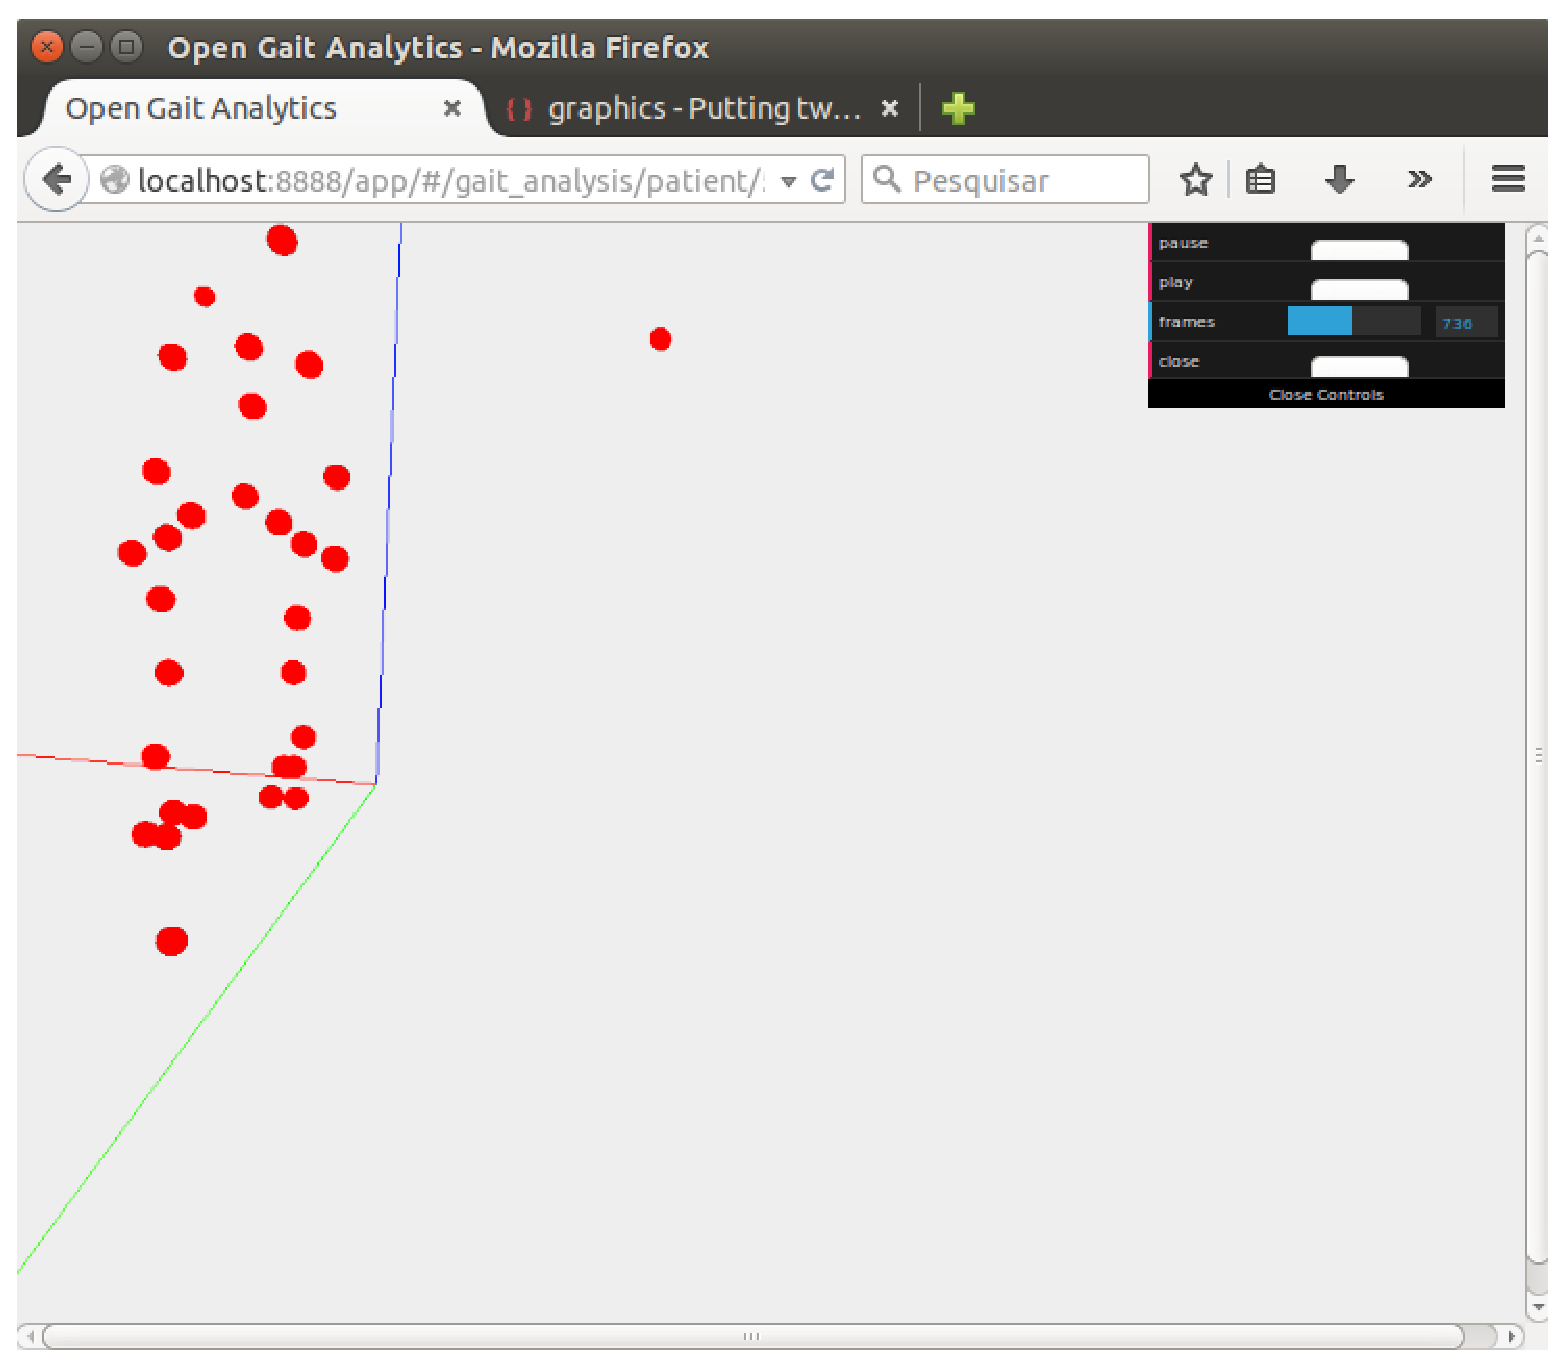
\includegraphics[width=\textwidth]{figuras/tela16.eps}
  \end{minipage}
  \caption{Controle \emph{pan}.}
  \label{animacao4}
\end{figure}

\begin{figure}[ht]
	\centering
	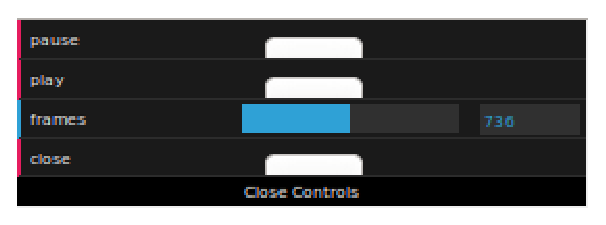
\includegraphics[width=7cm]{figuras/tela17.eps}
	\caption{Controles da animação.}
	\label{animacao5}
\end{figure}



\begin{figure}[ht]
	\centering
	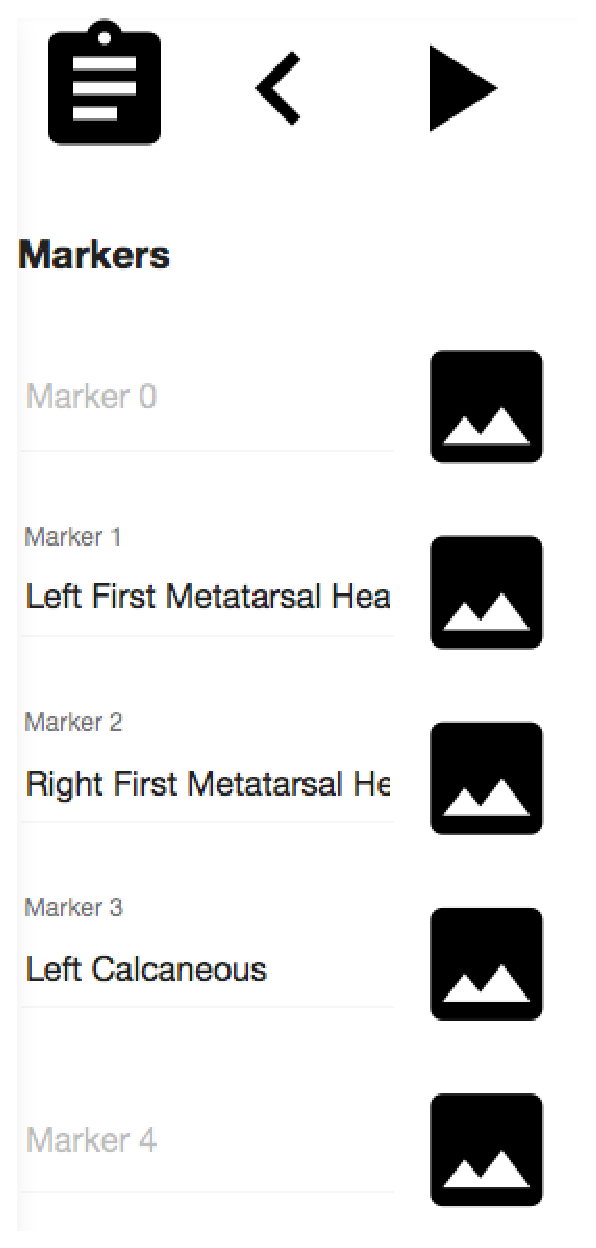
\includegraphics[width=5cm]{figuras/tela18.eps}
	\caption{Opção \emph{markers}.}
	\label{tela18}
\end{figure}


\begin{figure}[ht]
	\centering
	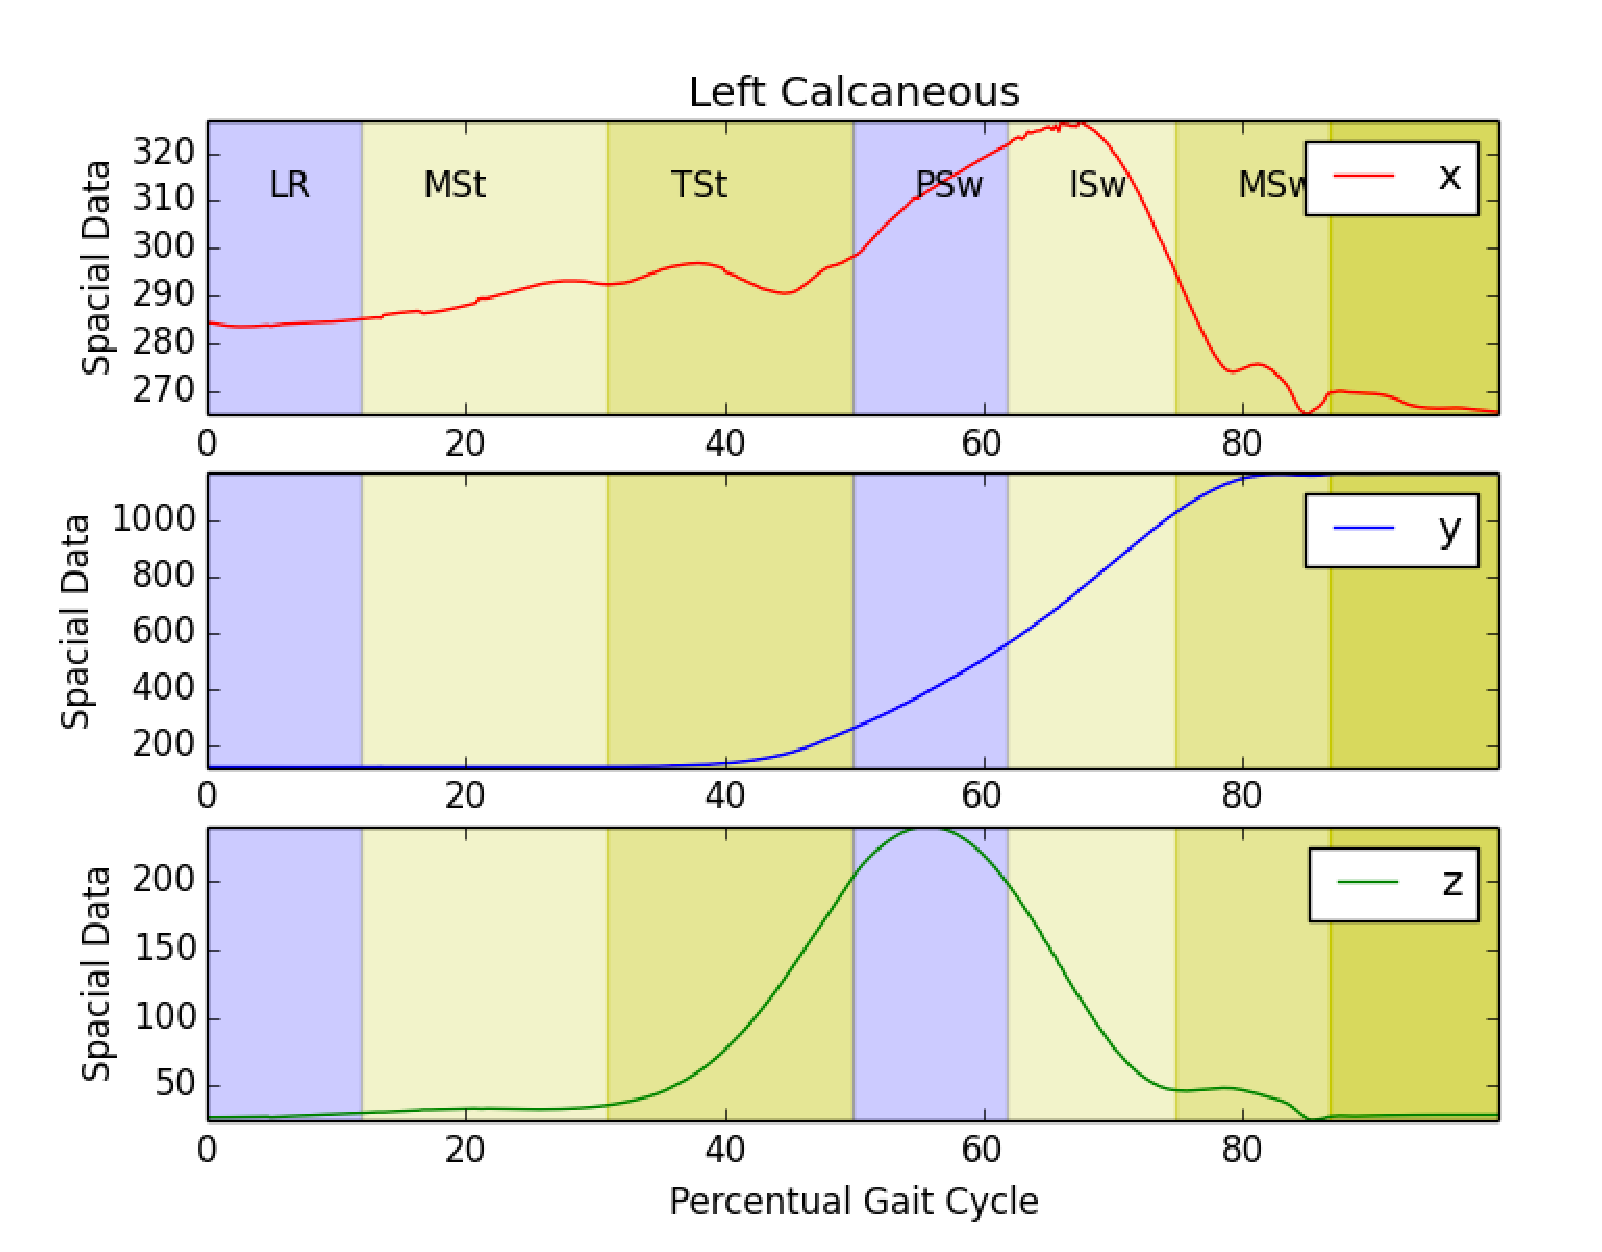
\includegraphics[width=10cm]{figuras/tela19.eps}
	\caption{Progreção espacial de um marcador.}
	\label{tela19}
\end{figure}

\begin{figure}[ht]
	\centering
	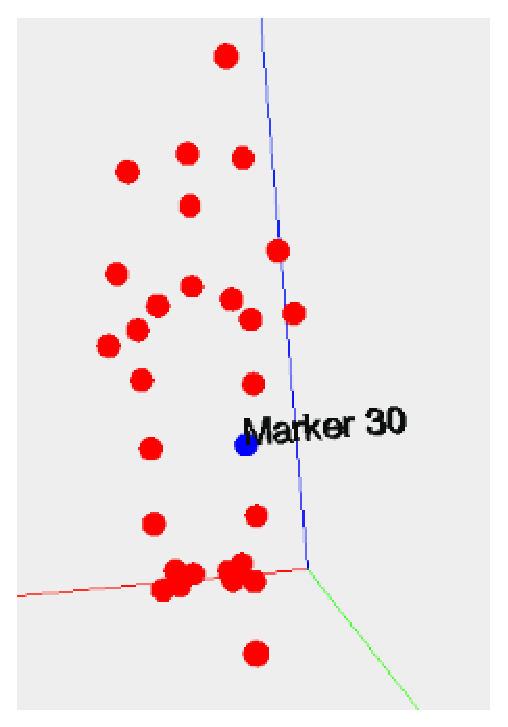
\includegraphics[width=5cm]{figuras/tela20.eps}
	\caption{Seleção de um marcador pelo \emph{mouse}.}
\label{tela20}
\end{figure}



\begin{figure}[ht]
	\centering
	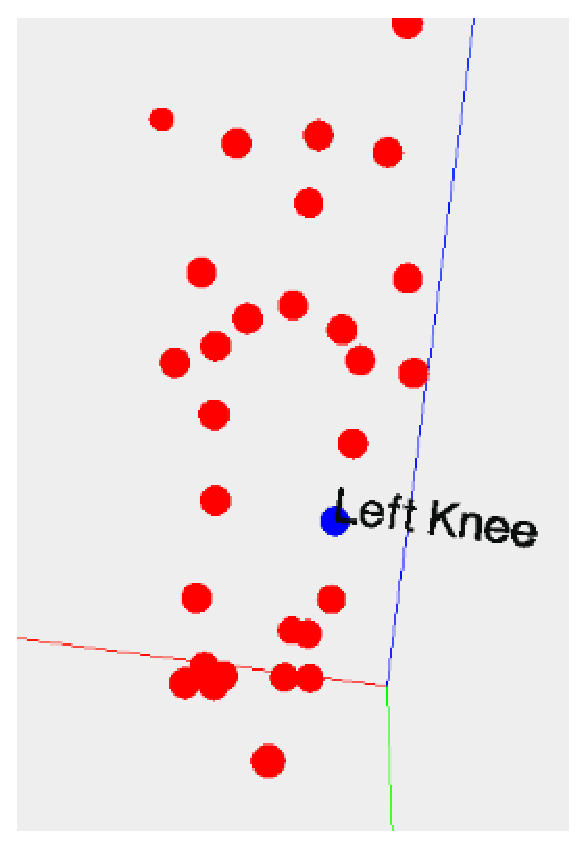
\includegraphics[width=5cm]{figuras/tela22.eps}
	\caption{Animação mostrando o marcador renomeado.}
\label{tela22}

\end{figure}


\begin{figure}[ht]
	\centering
	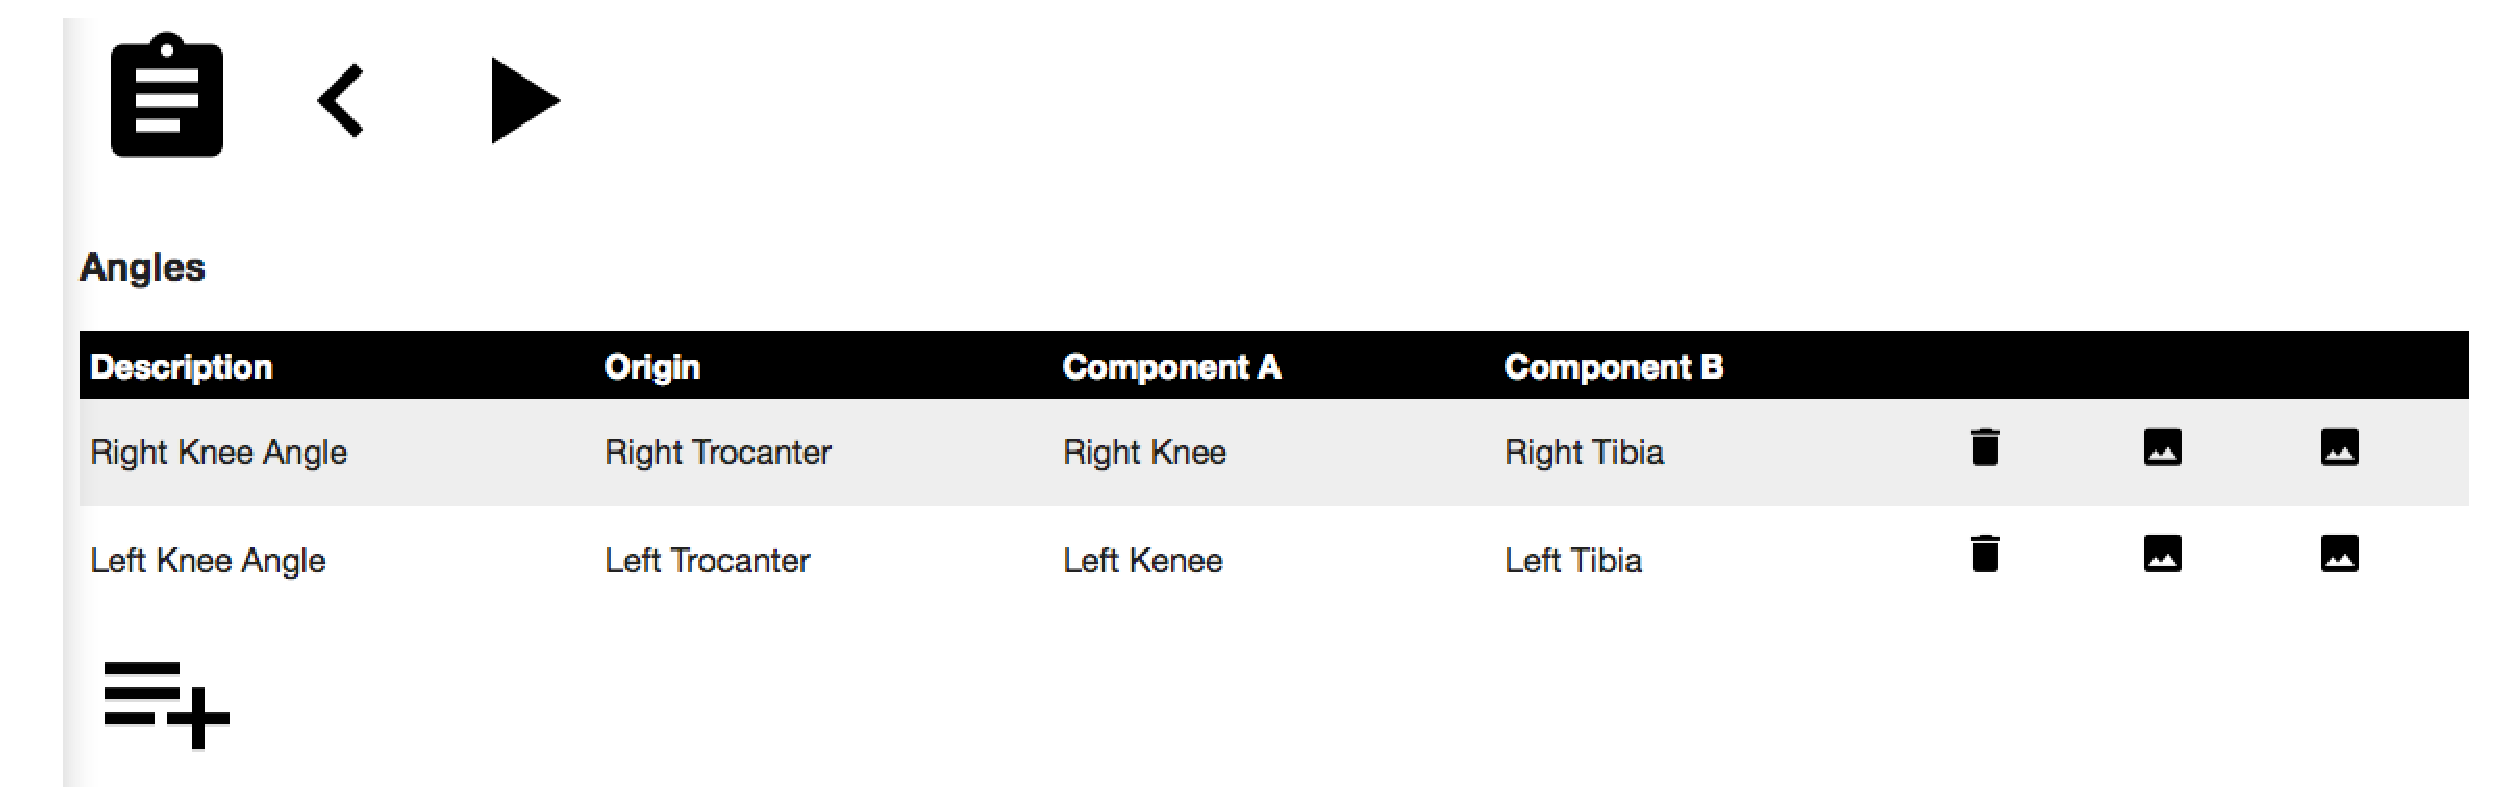
\includegraphics[width=15cm]{figuras/tela23.eps}
	\caption{Opção de visualização e criação de ângulos.}
\label{tela23}
\end{figure}


\begin{figure}[ht]
	\centering
	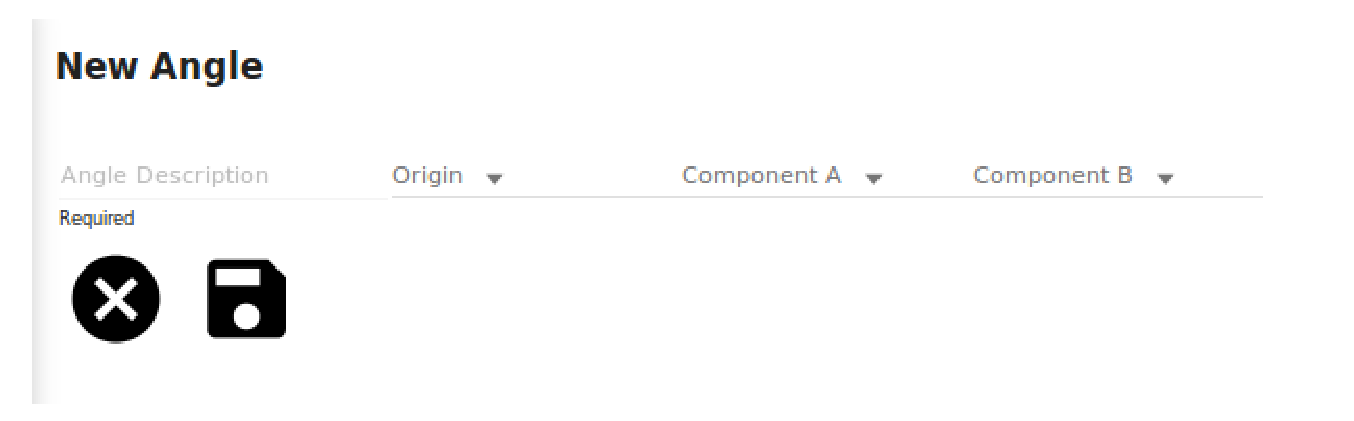
\includegraphics[width=15cm]{figuras/tela24.eps}
	\caption{Inclusão de um novo ângulo.}
\label{tela24}
\end{figure}

\begin{figure}[ht]
	\centering
	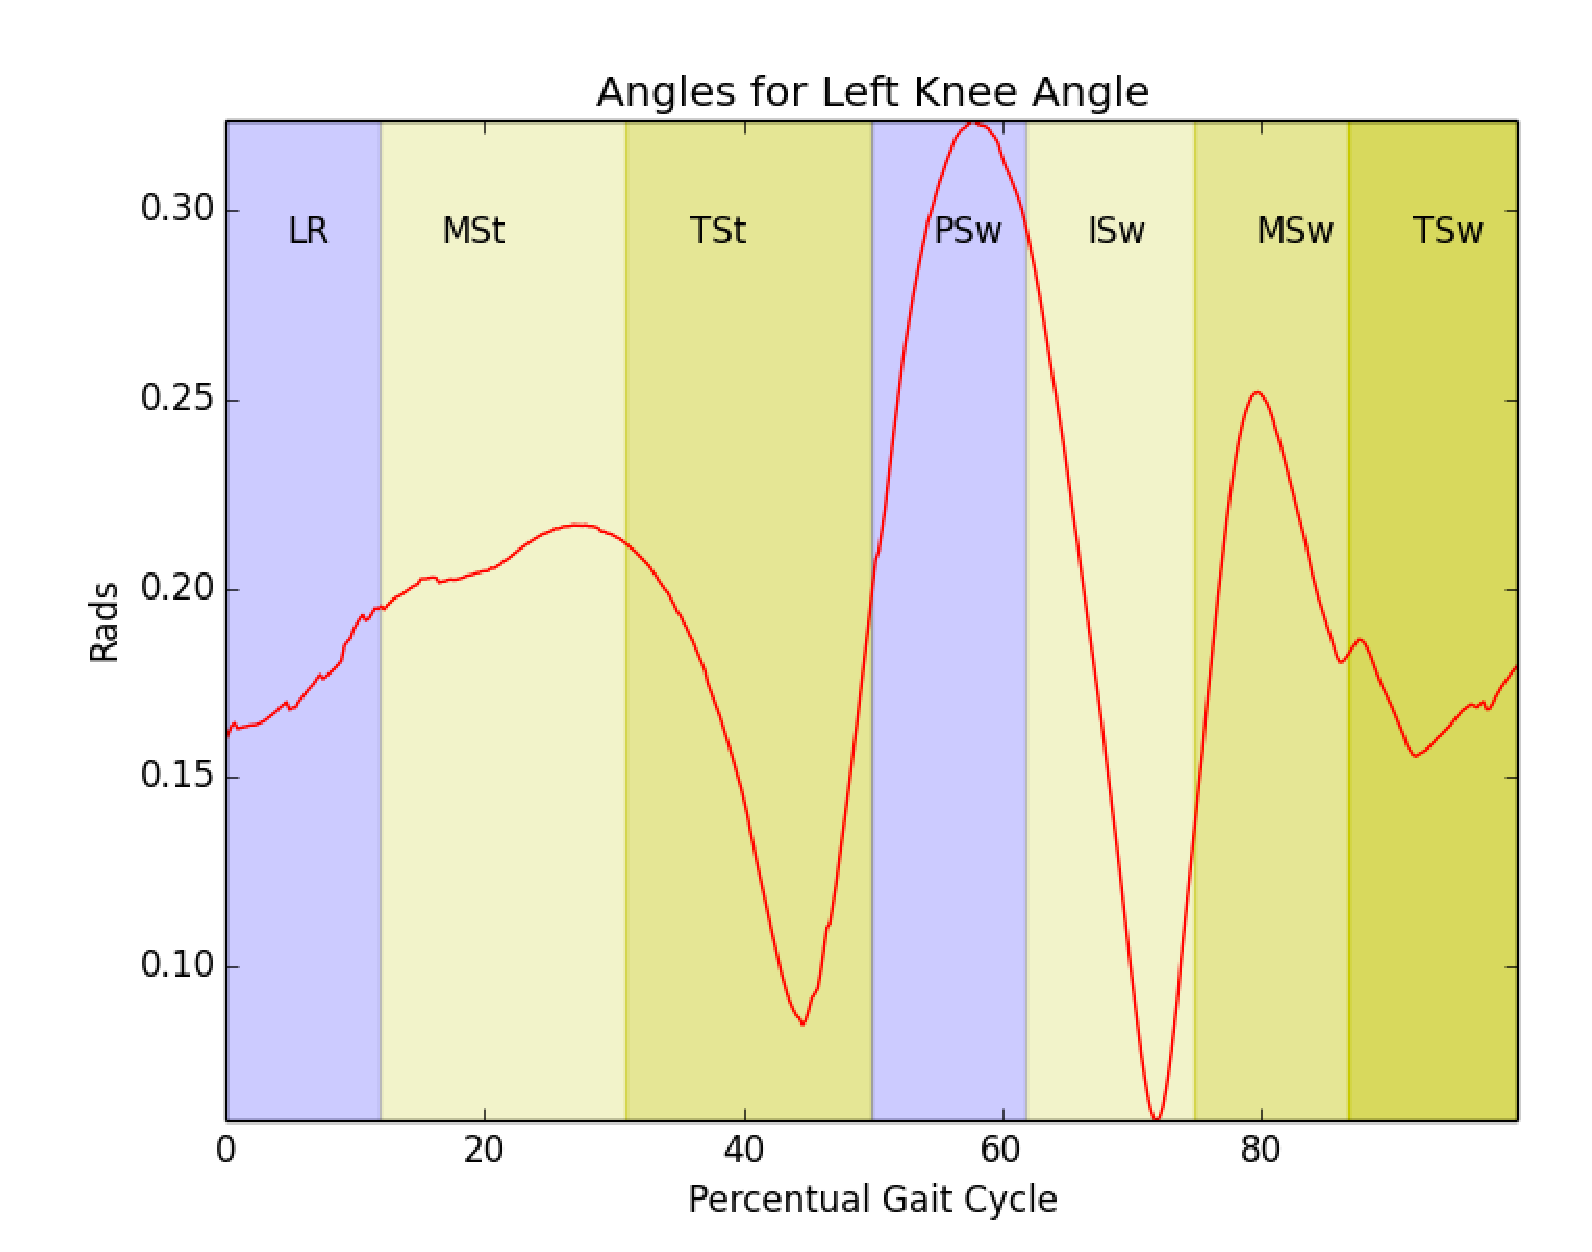
\includegraphics[width=10cm]{figuras/tela25.eps}
	\caption{Angulo de um joelho durante o ciclo de marcha.}
\label{tela25}
\end{figure}

\begin{figure}[ht]
	\centering
	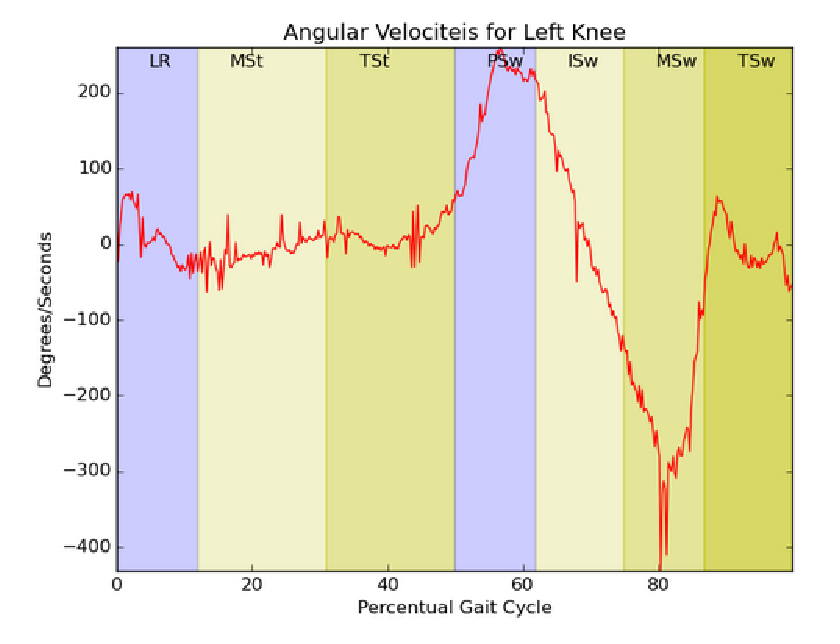
\includegraphics[width=10cm]{figuras/tela26.eps}
	\caption{Velocidades angulares de um joelho durante o ciclo de marcha.}
\label{tela26}
\end{figure}





\goodbreak
\newpage
\clearpage
\section{Módulo de Simulação}
Este módulo é sem dúvida o que mais vai contribuir para os pesquisadores, pois estes contarão com a base integrada gerada pelo módulo de análise e com estas informações será possível realizar simulações de sinais e classificações. 
A versão atual do software ainda é muito pobre neste quesito, mas o objetivo neste momento é mostra a viabilidade de se usar algoritmos de sistemas inteligentes, integrados na base que vai sendo gerada.
Acredita-se que a ferramenta vai ser mais apreciada por pesquisadores que tem como formação a área de saúde, pois estes não precisarão da parafernalha técnica exigida para fazer simulações num ambiente como o do \emph{MATLAB}.

O primeira funcionalidade de simulação que foi implentada foi a simulação pela \emph{CMAC}, esta RNA foi descrita na seção \ref{cmac_sec}. 
Ao se selecionar o módulo simulação a tela da Figura \ref{tela27} é apresentada. 
A opção \emph{CMAC}, já aparece selecionada. 
Para efeitos da demonstração das funcionalidades deste módulo será realizada uma simulação das velocidades angulares de um joelho, a partir de outros sinais disponíveis.

Após ser selecionado o nome de um paciente, deve-se selecionar uma amostra de ciclo de marcha, Figura \ref{tela28}.
Após a seleção do ciclo de marcha, uma lista com vários sinais são mostrados, basicamente os sinais são coordenadas de posições de marcadores, ângulos e velocidades angulares. As Figuras \ref{tela29} e \ref{tela30} mostram uma fração dos sinais possíveis para seleção. Ao se selicionar um sinal de entrada é necessário também informar sua quantização.

A Figura \ref{tela31} mostra uma configuração que gera a saída da figura \ref{tela32}. Infelizmente até o momento de escrita desta obra, não foi possível implementar a saída na aplicação. O gráfico mostrado é a saída de um protótipo desktop da \emph{CMAC} que usa os mesmos parâmetros de entradas mostrados na aplicação \emph{web}.
A figura \ref{tela33} mostra o erro quadrado médio da execução da simulação ao longo das iterações.

\begin{figure}[ht]
	\centering
	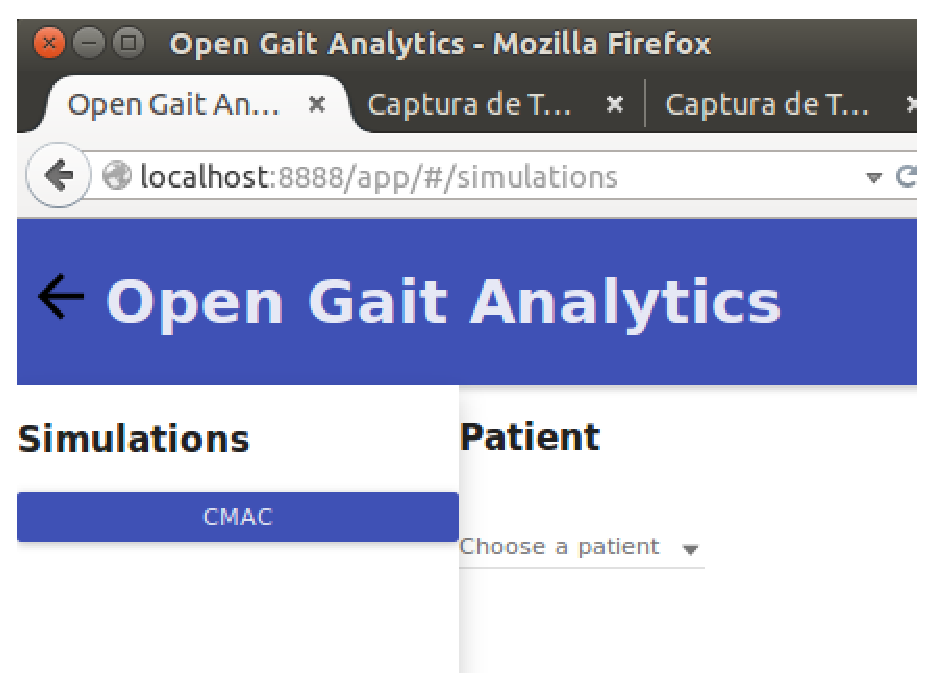
\includegraphics[width=10cm]{figuras/tela27.eps}
	\caption{Módulo de simulação.}
\label{tela27}
\end{figure}

\begin{figure}[ht]
	\centering
	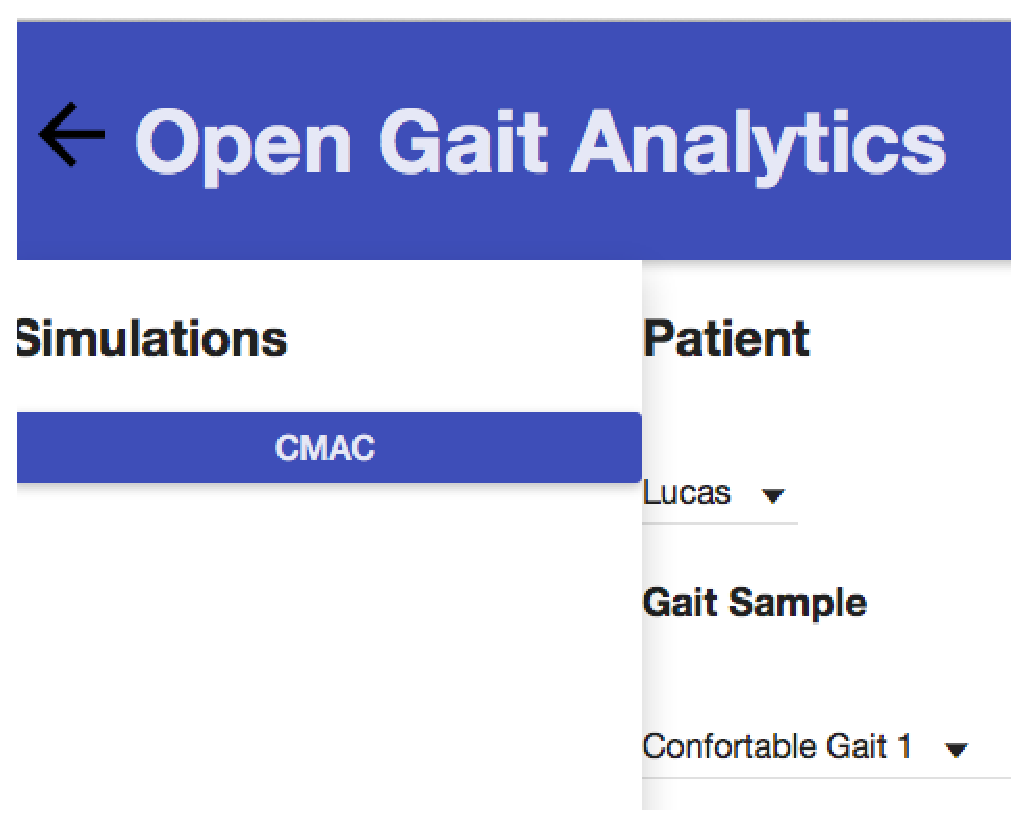
\includegraphics[width=10cm]{figuras/tela28.eps}
	\caption{Seleção do ciclo de marcha.}
\label{tela28}
\end{figure}

\begin{figure}[ht]
	\centering
	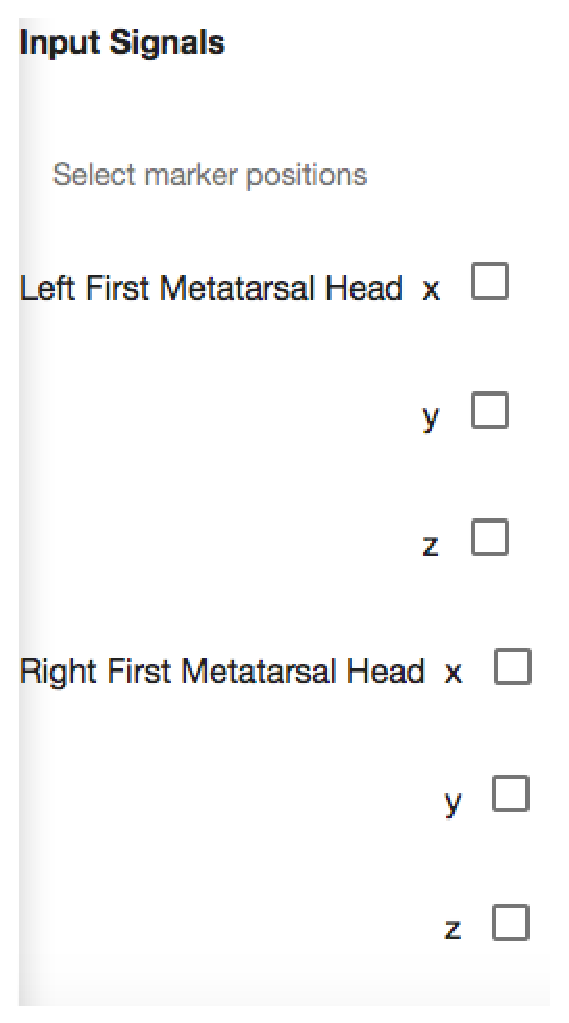
\includegraphics[width=5cm]{figuras/tela29.eps}
	\caption{Sinais de entrada para a \emph{CMAC}. No caso posições num plano 3D de marcadores.}
\label{tela29}
\end{figure}

\begin{figure}[ht]
	\centering
	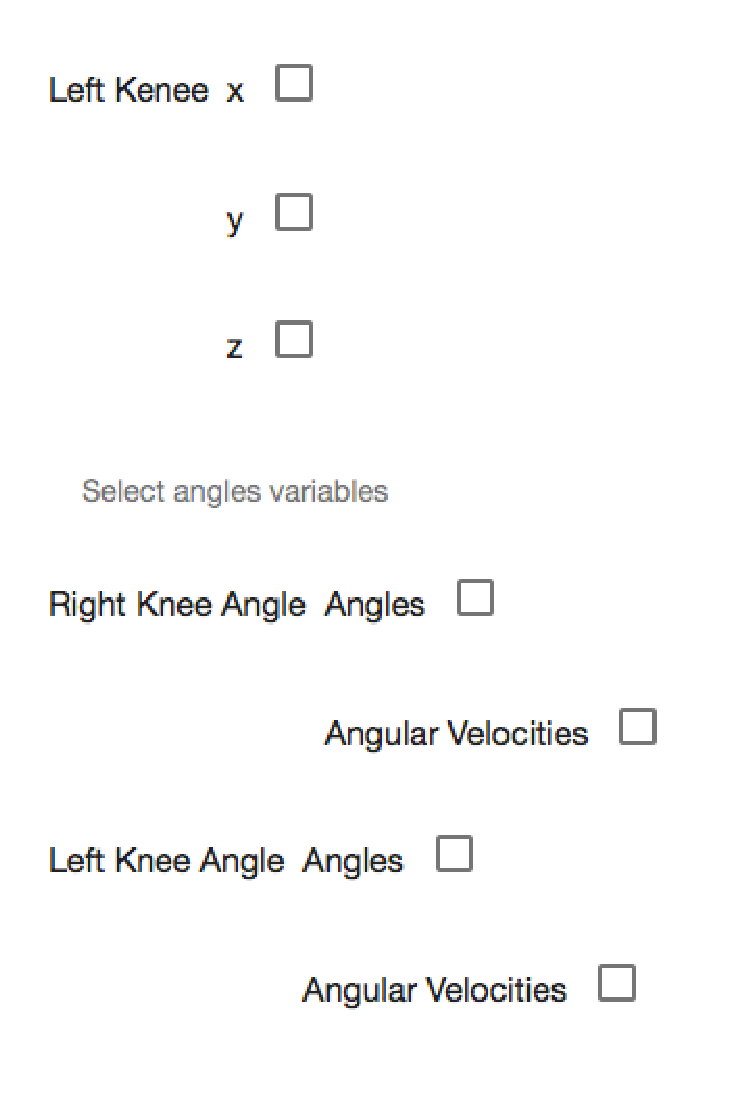
\includegraphics[width=5cm]{figuras/tela30.eps}
	\caption{Sinais de entrada para a \emph{CMAC}. Ângulos e velocidades angulares.}
\label{tela30}
\end{figure}

\begin{figure}[ht]
	\centering
	\includegraphics[width=10cm]{figuras/tela31.eps}
	\caption{Exemplo de configuração para uma simulação usando \emph{CMAC}.}
\label{tela31}
\end{figure}

\begin{figure}[ht]
	\centering
	\includegraphics[width=10cm]{figuras/tela32.eps}
	\caption{Resultado da simulação.}
\label{tela32}
\end{figure}

\begin{figure}[ht]
	\centering
	\includegraphics[width=10cm]{figuras/tela33.eps}
	\caption{Erro quadrado médio em cada iteração da simulação}
\label{tela33}
\end{figure}



\chapter[DISCUSSÃO E CONCLUSÃO]{\textbf{DISCUSSÃO E CONCLUSÃO}}

Há vários softwares de análise marcha no mercado, mas a ideia de criar um totalmente na \emph{web} tem suas vantagens. 
A mais óbvia é disponibilidade, já que a aplicação fica num servidor na internet, o usuário só precisa acessar um site com um browser. 
Outra não tão óbvia e que diz respeito principalmente ao módulo de simulação, é possibilidade de escalar a aplicação para necessidades de processamento gigantescas, usando infraestrutura como serviço de fornecedores como o \emph{Microsoft Azure} ou \emph{Amazon Webservices}.
Como a camada \emph{web} se comunica via \emph{HTTP} no estilo \emph{REST}, usando uma \emph{facade} para isto, basta fazer a \emph{facade} do módulo de simulação para uma \emph{web farm} alocada sob demanda num dos serviços mencionados. A vantagem óbvia é que quem serve a aplicação, pode alocar estes serviços sob demanda, não necessitando possuir um CPD caríssimo. O custo é repassado ao cliente que deseja usar os serviços de simulação que demandam muito poder de processamento.

Outro ponto interessante com a implantação da aplicação é a criação de uma base de dados de marcha humana, que pode receber dados de todo o globo. 
As vantagens para pesquisadores seriam inimagináveis.

Claro que nada disto é gratuito, os responsáveis pelo projeto terão de almejar meios para produzi-lo, achar nichos de mercado e colocá-lo em produção.

Ressalta-se novamente, que o software que está sendo entregue não está pronto para produção, o prazo disponível para desenvolvê-lo, inclusive adquirindo conhecimentos sobre muitas das tecnologias adotadas, foi de aproximadamente cinco meses. Isto ocorreu por que durante o programa de mestrado resolveu-se mudar o tema, devido a uma série de intempéries. No entanto, o software foi feliz em mostrar a integração de vários componentes nas diferentes camadas da aplicação. Esse estresse arquitetural é muito importante para se avaliar a viabilidade técnica de um projeto de engenharia de software.

Outro problema com o software entregue, é seu modesto poder de processamento com relação a simulações. 
Facilmente uma simulação em grande um \emph{Data Center} poder demorar dias. 
A solução para este problema é desenvolver um método de disparar a simulação assincronamente, e criar uma tela de gestão da execução da mesma. 
Para isso o software terá de ser integrado a componentes de computação distribuída como \emph{Apache Spark} ou o \emph{Hadoop}, fazendo uso de infraestrutura como serviço como mencionado acima. 
O potencial para este projeto se tornar algo inovador e principalmente muito útil na área de marcha humana é imenso.

Talvez o objetivo que tenha sido mais prejudicado, foi a implantação do método ágil. 
Como o método escolhido, foi o \emph{SCRUM} e não foi possível criar as reuniões diárias \emph{(daily scrum)}, a dinâmica da equipe não foi a mesma em que o autor teve a oportunidade de trabalhar com outras equipes.
Recomenda-se também, que uma equipe de especialistas clínicos e pesquisadores da área da marcha humana sejam adicionados ao projeto e ajudem ao \emph{product owner} do projeto a definir novas funcionalidades para o sistema. 
A questão dos testes também foi um pouco prejudicada, mas não abandonada, na verdade esta foi uma escolha do autor, que devido ao pouco tempo para desenvolvimento, preferiu dar ênfase na produção de novas características. Mesmo assim todos os principais componentes, como a \emph{web API} e os componentes de telas da análise de marcha possuem testes automatizados.
A consequência é que \emph{bugs} menores como listas de seleção podem aparecer fora dos locais adequados, o componente de controle de animação as vezes fica com um tamanho inadequado, mas não é nada que com os recursos adequados não se resolva.

Isso certamente vai acelerar a adoção do software por estes profissionais, já que são as necessidades deles que serão atingidas.
Talvez um projeto de \emph{crowdfunding} possa trazer estes profissionais. 
É comum nestes projetos os clientes pedirem funcionalidades para o software.
O problema é que este é um software para um nicho muito especializado, pode ser que não seja uma boa ideia.

Vale lembra também que o projeto não vai se limitar a análise de movimento, outros métodos de coleta de dados para análise serão inseridos ao longo do tempo.


Concluindo, os objetivos foram alcançados, foi definida uma metodologia ágil, foi criado um modelo de arquitetura, um software foi construído, integrado com os principais componentes e na medida do possível testados, e mais uma vez, frisando que toda a arquitetura foi estressada. 
Além disso a aplicação ainda apresenta características para serem executadas em dispositivos móveis. 
Também o código fonte com todo o histórico de desenvolvimento do projeto esta no site \url{https://github.com/rob-nn/open\_gait\_analytics}, lembrando que o código está sob licença MIT, e qualquer um pode usá-lo como bem entendê-lo.


\chapter[TRABALHOS FUTUROS]{\textbf{TRABALHOS FUTUROS}}
Como este foi um projeto com um intuito de plantar uma semente, não faltarão trabalhos futuros para complementá-lo, aumentá-lo ou mesmo expândi-lo para outras áreas além da análise de marchar.
\begin{enumerate}
	\item O trabalho mais urgente a ser feito é pegar a versão atual, testá-la o máximo possível, corrigir os bugs encontrados e disponibilizá-la na web;
	\item Criar um módulo de usuários e instituições;
	\item Criar um filtro para retirar ruídos da animação;
	\item Inserir o padrão ouro nos gráficos para efeito de comparação;
	\item Incluir um controle do tipo \emph{slide} para controlar a animação;
	\item Criar o componente de animação como uma diretiva do \emph{angular-js}, para reutilização em outros pontos do projeto;
	\item Criar no módulo de simulação uma ferramenta para modelagem de sinais de entrada, métodos de processamento e sinais de saída, baseados nos dados da base de documentos;
	\item Permitir adicionar e visualizar foto do paciente;
	\item Permitir adicionar e visualizar vídeos das amostras de marcha coletadas;
	\item Habilitar o protocolo \emph{HTTP Auth} nas requisições feitas a \emph{web API};
	\item Habilitar protocolo \emph{HTTPS} entre servidor \emph{web} e \emph{browser} cliente;
	\item Utilizar um componente do tipo \emph{data picker} nos campos de datas;
	\item Implementar um detector automático de ciclo de marchar, assim não será necessário o usuário informar o início e fim do ciclo;
	\item Permitir cadastrar protocolos de coleta por câmeras e fazer a detecção automática dos mesmos, assim o usuário não necessitará nomear marcadores;
	\item Permitir coletar dados de plataforma de força e criar gráficos;
	\item Permitir coletar dados de \emph{IMUs} e criar gráficos;
	\item Permitir coletar dados de \emph{EMGs} e criar gráficos;
	\item Permitir coletar dados de eletrogoniômetros;
	\item Criar suporte a várias língua, começando com português e inglês;
	\item Implementar outros algoritmos de sistemas inteligentes, como \emph{PCA}, \emph{Kmeans}, \emph{SVM}, \emph{MLP}, entre outros, integrando estes algoritmos a ferramenta de modelagem de sinais, permitindo se fazer classificações e regressões. Por exemplo, usando-se \emph{SVM} é possível fazer a detecção de quedas, ou usando o Kmeans é possível detectar os momento distintos no uso de uma plataforma de força. Aqui o que vai imperar é a criatividade do pesquisador, que terá nas mãos uma ferramenta visual para fazer estas simulações. A evolução desse módulo acontecerá quando a simulações forem úteis o suficiente para auxiliar nos diagnósticos de patologias na marcha. Com a tecnologia atual de aprendizado de máquina, as possibiliades são muito atrativas.
	\item Integrar o módulo de simulação com plataformas de infraestrutura com serviço, usando para isso ferramentas como Hadoop ou Spark;
	\item Tornar a função de execução de simulações assíncronas;
	\item Criar um módulo gestor da execução das simulações, com opções de parar, pausar, continuar, alocar mais recursos, enfileiramento.
\end{enumerate}




\bookmarksetup{startatroot} 
\postextual

\renewcommand{\bibname}{\textbf{REFERÊNCIAS BIBLIOGRÁFICAS}} % Altera o nome da Referêcia para Referêcia Bibliográfica
\bibliography{bibliografia}

% ----------------------------------------------------------
% Anexos
% ----------------------------------------------------------

% ---
% Inicia os anexos
% ---
\begin{anexosenv}

% Imprime uma página indicando o início dos anexos
\partanexos

% ---
\chapter{PROCESSO NO COMITÊ DE ÉTICA}
% ---
\label{comite_sec}
\begin{figure}[ht]
	\centering
	\includegraphics[width=15cm]{figuras/comite.eps}
	\caption{Processo no comitê de ética.}
\label{comite}
\end{figure}


\end{anexosenv}


\printindex

\end{document}
